\chapter*{INTRODUCTION}
\addcontentsline{toc}{chapter}{\textbf{INTRODUCTION}}
Trong sự phát triển nhanh chóng của các hệ thống truyền thông hiện đại như mạng 5G/6G, Internet of Things (IoT), mạng cảm biến không dây, liên kết vệ tinh và hệ thống liên lạc quân sự, nhu cầu truyền dữ liệu đáng tin cậy, tốc độ cao và độ trễ thấp ngày càng trở nên quan trọng. Trong thực tế, tín hiệu được truyền qua kênh vật lý bị ảnh hưởng bởi nhiều yếu tố bất lợi, bao gồm nhiễu ngẫu nhiên, truyền đa đường, pha đinh, lỗi cụm, đồng bộ hóa không khớp, méo phần cứng phi tuyến và các dạng không chắc chắn khác không phải lúc nào cũng được mô hình hóa chính xác. Trong những điều kiện này, mã hóa kênh vẫn là một trong những kỹ thuật quan trọng nhất để cải thiện độ tin cậy truyền dẫn và giảm xác suất mất thông tin~.

Nền tảng lý thuyết về giao tiếp đáng tin cậy được Claude Shannon thiết lập vào năm 1948 \cite{shannon1948}. Công trình của Shannon cho thấy rằng, dưới dung lượng kênh, khả năng liên lạc đáng tin cậy có thể thực hiện được khi sử dụng các sơ đồ mã hóa phù hợp. Kể từ đó, nhu cầu ngày càng tăng về hiệu quả băng thông, độ tin cậy và tốc độ dữ liệu đã thúc đẩy nghiên cứu sâu rộng về sửa lỗi chuyển tiếp, Điều chế bậc cao và xử lý máy thu lặp. Các hệ thống truyền thông hiện đại không dựa vào một kỹ thuật biệt lập duy nhất. Thay vào đó, chúng kết hợp mã hóa kênh, Điều chế, Giải điều chế, xen kẽ và xử lý thông tin mềm để tiếp cận các giới hạn hiệu suất do kênh vật lý áp đặt.

Để cải thiện hiệu suất phổ, nhiều cấu trúc điều chế mã hóa kết hợp Điều chế bậc cao với mã hóa kênh. Một cấu trúc tiêu biểu và được nghiên cứu rộng rãi là Điều chế mã hóa xen kẽ bit với giải mã lặp (BICM-ID) \cite{caire1998,li1997,li1998}. So với BICM thông thường, BICM-ID giới thiệu sự trao đổi lặp lại thông tin bên ngoài giữa khối Giải điều chế mềm và bộ giải mã kênh. Cơ chế này cho phép máy thu tinh chỉnh các giá trị độ tin cậy của bit qua nhiều lần lặp và có thể cải thiện đáng kể hiệu suất tỷ lệ lỗi bit khi nhãn Điều chế, xen kẽ và mã kênh được thiết kế nhất quán. Ngoài ra, các chòm sao bậc cao như $M$-QAM cho phép truyền nhiều bit hơn trên mỗi ký hiệu, từ đó cải thiện việc sử dụng băng thông. Sự tách biệt giữa mã hóa kênh và ánh xạ tín hiệu cũng mang lại tính linh hoạt cho BICM-ID vì các mã và chòm sao khác nhau có thể được kết hợp trong cùng một nguyên tắc máy thu.

Điều chế mã hóa xen kẽ bit xen kẽ với giải mã lặp lại (BIBCM-ID) tuân theo triết lý thông tin mềm tương tự trong khi nhấn mạnh vai trò của khối hoặc xen kẽ bit trong việc kiểm soát mối quan hệ giữa vị trí bit được mã hóa và vị trí bit điều chế. Một hệ thống BIBCM-ID có thể được xem qua ba thành phần thiết yếu: Điều chế và Giải điều chế, mã hóa và giải mã kênh và bộ xen kẽ. Quá trình điều chế xác định hình dạng của tín hiệu được truyền và ghi nhãn bit của các điểm chòm sao. Mã hóa kênh cung cấp sự dự phòng có cấu trúc để sửa lỗi. Bộ chèn xen kẽ trải rộng các bit được mã hóa trên các vị trí ký hiệu, giảm mối tương quan có hại và hỗ trợ việc trao đổi lặp đi lặp lại các thông tin bên ngoài. Các nghiên cứu gần đây về thiết kế bộ xen đã tạo ra những kết quả mạnh mẽ về bộ xen đại số, bộ xen ngẫu nhiên S, cấu trúc nhận biết sơ đồ và bộ xen hướng hướng phần cứng. Vì vậy, luận án này coi bộ xen kẽ là một thành phần quan trọng được thiết lập và tập trung vào hai hướng còn lại: bộ giải mã kênh LDPC và giao diện Điều chế/Giải điều chế.

Trong luận án này, thuật ngữ BIBCM-ID được sử dụng để biểu thị việc thực hiện nguyên tắc BICM-ID theo khối xen kẽ. Nó không đưa ra nguyên tắc giải mã xác suất khác với BICM-ID; đúng hơn, nó làm cho bộ xen kẽ khối và ảnh hưởng của nó lên mối quan hệ bit mã hóa/bit điều chế trở nên rõ ràng. Sự khác biệt này rất hữu ích vì nghiên cứu hiện tại thảo luận về bộ thu như một chuỗi các giao diện thông tin mềm, trong đó bộ xen kẽ khối là một thành phần hệ thống nhưng không phải là đối tượng chính của tối ưu hóa mạng thần kinh.

Mặc dù BICM-ID và BIBCM-ID cung cấp một khung hiệu quả nhưng hiệu suất của chúng phụ thuộc rất nhiều vào mã kênh, sơ đồ Điều chế, chất lượng Giải điều chế mềm và độ phức tạp tính toán của giải mã lặp. Các mã kênh hiện đại như mã chập, mã Turbo, mã LDPC và mã Polar cung cấp khả năng sửa lỗi mạnh mẽ, nhưng chúng cũng đưa ra những thách thức về tính toán và độ trễ. Mã LDPC đặc biệt quan trọng vì chúng có ma trận kiểm tra chẵn lẻ thưa thớt và có thể được giải mã hiệu quả bằng cách truyền thông báo trên biểu đồ Tanner \cite{gallager1962,mackay1996,richardson2008}. Tuy nhiên, Thuật toán tổng sản phẩm (SPA), là phương pháp giải mã LDPC xác suất cổ điển, chứa các hoạt động nút kiểm tra phi tuyến tính liên quan đến các hàm hyperbol. Các thuật toán đơn giản hóa như Min-Sum làm giảm độ phức tạp nhưng có thể làm giảm hiệu suất. Sự cân bằng này thúc đẩy việc sử dụng mạng nơ-ron nhân tạo làm công cụ xấp xỉ hàm nhỏ gọn cho các hoạt động phi tuyến được chọn bên trong bộ giải mã LDPC.

Trong những năm gần đây, deep learning cũng đã được nghiên cứu để phục vụ cho việc giao tiếp ở lớp vật lý. Các phương pháp truyền bá niềm tin thần kinh, các hiệu chỉnh Min-Sum đã học và bộ giải mã thần kinh dựa trên mô hình cho thấy rằng mạng thần kinh có thể được đưa vào giải mã lặp trong khi vẫn giữ nguyên cấu trúc mã \cite{nachmani2016,nachmani2018,kuck2020,wang2022}. Đồng thời, hệ thống liên lạc dựa trên AutoEncoding cho thấy máy phát và máy thu có thể được đào tạo chung để tìm hiểu các cách biểu diễn tín hiệu phù hợp với điều kiện kênh \cite{oshea2017,dorner2018,aoudia2019}. Những phát triển này cho thấy mạng lưới thần kinh có thể hữu ích không phải là sự thay thế cho lý thuyết truyền thông mà là công cụ để xấp xỉ các hàm phi tuyến, sửa lỗi mô hình không khớp, giảm độ phức tạp khi triển khai và cải thiện chất lượng thông tin mềm.

Xuất phát từ những động cơ trên, luận án này nghiên cứu ứng dụng mạng nơ-ron nhân tạo trong giải mã LDPC cho các hệ thống truyền thông định hướng BIBCM-ID. Trọng tâm kỹ thuật trọng tâm là bộ giải mã kênh LDPC, đặc biệt là điều chỉnh gần đúng và nhận biết độ tin cậy của các thông báo nút kiểm tra trong giải mã lan truyền niềm tin lặp đi lặp lại. Luận án cũng nghiên cứu Điều chế dựa trên AutoEncode như một hướng bổ sung liên quan đến giao diện Điều chế/Giải điều chế~. Phần này được bao gồm vì bộ giải mã LDPC trong bộ thu BIBCM-ID hoạt động dựa trên thông tin mềm do khối Giải điều chế tạo ra. Nếu các suy giảm kênh như phi tuyến của bộ khuếch đại công suất, độ lệch tần số sóng mang, pha đinh và nhiễu phụ làm biến dạng chòm sao nhận được thì Giải điều chế thông thường có thể tạo ra LLR sai lệch hoặc hiệu chỉnh kém. Do đó, mô hình Điều chế/Giải điều chế đã học có liên quan như một nghiên cứu hỗ trợ về nguồn thông tin mềm cung cấp cho Bộ giải mã LDPC~.

Mục tiêu nghiên cứu là đánh giá nơi mạng lưới thần kinh nhân tạo có thể được đưa vào máy thu định hướng BIBCM-ID mà không từ bỏ các nguyên tắc đã được thiết lập về điều chế mã hóa và giải mã lặp. Trong phần giải mã LDPC, luận án phân tích cơ sở toán học của việc lan truyền niềm tin, cập nhật nút kiểm tra, xấp xỉ Min-Sum và sử dụng mạng nơ ron nhỏ gọn để xấp xỉ hoặc điều chỉnh thông báo nút kiểm tra. Trong phần Điều chế, luận án phân tích ánh xạ tín hiệu dựa trên AutoEncode trong các điều kiện kênh không lý tưởng và làm rõ Điều chế và Giải điều chế đã học có thể ảnh hưởng như thế nào đến độ tin cậy của các giá trị LLR. Nghiên cứu được thực hiện thông qua phân tích lý thuyết, kết quả mô phỏng được báo cáo trong luận án này và thảo luận có kiểm soát về độ phức tạp tính toán và chất lượng thông tin mềm~.

Luận văn bao gồm ba chương chính. Chương 1 trình bày nền tảng của BIBCM-ID, bao gồm chuỗi điều chế mã hóa, Giải điều chế mềm, trao đổi lặp lại thông tin bên ngoài, mã hóa kênh và vai trò của việc xen kẽ. Chương này cũng xác định phạm vi nghiên cứu và giải thích vì sao luận án tập trung vào giải mã LDPC và Điều chế/Giải điều chế hơn là đề xuất thiết kế bộ xen mới. Chương 2 phân tích deep learning cho Điều chế và Giải điều chế thông minh. Nó thảo luận về các mô hình truyền thông AutoEncode, tính phi tuyến PA, CFO, độ mờ, hình học tín hiệu đã học, hiệu chuẩn LLR và kết nối giữa Giải điều chế đã học và đầu vào bộ giải mã LDPC. Chương 3 nghiên cứu giải mã LDPC với sự hỗ trợ của ANN. Nó xem xét việc truyền thông báo LDPC, cập nhật nút kiểm tra SPA và Min-Sum, phép tính gần đúng thần kinh nhỏ gọn của chức năng nút kiểm tra, chiến lược nhãn huấn luyện, đánh giá độ phức tạp và diễn giải kết quả BER.

Với định hướng này, luận án nhằm mục đích cung cấp một phân tích có hệ thống về cách các kỹ thuật mạng thần kinh có thể hỗ trợ giải mã LDPC và xử lý thông tin mềm liên quan trong các hệ thống định hướng BIBCM-ID. Đóng góp được mong đợi không phải là sự thay thế rộng rãi các khối truyền thông cổ điển bằng mạng thần kinh hộp đen, mà là một cách tiếp cận có cấu trúc trong đó các mô hình lý thuyết truyền thông được giữ lại và mạng thần kinh được sử dụng khi chúng được chứng minh về mặt kỹ thuật: xấp xỉ nút kiểm tra phi tuyến tính, kiểm soát độ tin cậy và phân tích Điều chế/Giải điều chế nhận biết kênh.

Trong thời gian hoàn thành luận văn thạc sĩ này, tác giả đã nhận được sự giúp đỡ quý báu từ các giảng viên và đồng nghiệp tại Khoa Điện tử vô tuyến, Học viện Kỹ thuật Quân sự. Tác giả xin bày tỏ lòng biết ơn chân thành đến người hướng dẫn khoa học là Tiến sĩ Phạm Xuân Nghĩa và Tiến sĩ Hoàng Văn Dũng đã hướng dẫn, nhận xét và hỗ trợ trong suốt quá trình nghiên cứu. Tác giả cũng đánh giá cao những phản hồi mang tính xây dựng của thầy cô, đồng nghiệp và các bạn sinh viên, giúp hoàn thiện nội dung kỹ thuật và cách trình bày luận án.

\chapter[\textbf{NỀN TẢNG BIBCM-ID VÀ PHẠM VI NGHIÊN CỨU}]{NỀN TẢNG BIBCM-ID VÀ PHẠM VI NGHIÊN CỨU DỰA TRÊN HỌC TẬP}
\section{Mô hình hệ thống truyền thông kỹ thuật số}
Hệ thống truyền thông kỹ thuật số truyền chuỗi thông tin từ nguồn đến đích thông qua kênh vật lý. Trong mô hình băng cơ sở đơn giản hóa, nguồn tạo ra chuỗi bit $\mathbf{u}$, bộ phát chuyển đổi chuỗi này thành dạng sóng hoặc chuỗi ký hiệu kênh và bộ thu ước tính thông tin được truyền từ các quan sát nhiễu. Mục tiêu kỹ thuật chính là giảm xác suất xảy ra lỗi trong khi vẫn đáp ứng các ràng buộc về băng thông, công suất truyền, độ trễ và độ phức tạp khi triển khai.

Chuỗi tín hiệu cơ bản được minh họa trong Hình~\ref{fig:digital_comm_system}. Mã hóa kênh bổ sung tính dự phòng để bảo vệ các bit thông tin, Điều chế ánh xạ các bit tới các điểm tín hiệu vật lý và Giải điều chế chuyển đổi các mẫu nhận được thành các quyết định bit hoặc giá trị độ tin cậy. Do đó, việc tiếp nhận đầu ra mềm cung cấp cả ước tính bit và giá trị độ tin cậy cho việc giải mã tiếp theo.

\begin{figure}[H]
\centering
\resizebox{0.96\textwidth}{!}{%
\begin{tikzpicture}[
  block/.style={draw, align=center, minimum height=0.90cm, text width=1.85cm, font=\footnotesize},
  terminal/.style={draw, rounded corners=0.38cm, align=center, minimum height=0.62cm, text width=1.38cm, font=\footnotesize},
  line/.style={-{Latex[length=2mm]}, thick},
  note/.style={font=\scriptsize, align=center}
]
\node[terminal] (source) at (0,0) {Source};
\node[block] (senc) at (2.35,0) {Source\\Encoder};
\node[block] (cenc) at (5.85,0) {Channel\\Encoder};
\node[block] (mod) at (9.45,0) {Modulator};
\node[block] (channel) at (10.95,-1.45) {Channel};
\node[block] (demod) at (9.45,-2.90) {Demodulator};
\node[block] (cdec) at (5.85,-2.90) {Channel\\Decoder};
\node[block] (sdec) at (2.35,-2.90) {Source\\Decoder};
\node[terminal] (recv) at (0,-2.90) {Receiver};

\draw[line] (source) -- (senc);
\draw[line] (senc) -- (cenc);
\draw[line] (cenc) -- node[note, above] {$X$} (mod);
\draw[line] (mod.east) -- ++(0.60,0) |- (channel.north);
\draw[line] (channel.south) |- (demod.east);
\draw[line] (demod) -- node[note, above] {$Y$} (cdec);
\draw[line] (cdec) -- (sdec);
\draw[line] (sdec) -- (recv);

\draw[densely dotted, thick] (7.75,0.80) rectangle (12.30,-3.55);
\node[note, font=\footnotesize] at (10.05,1.08) {Equivalent Discrete channel};
\end{tikzpicture}
}
\caption{Cấu trúc cơ bản của hệ thống truyền thông số.}
\label{fig:digital_comm_system}
\end{figure}

Đối với kênh băng cơ sở phức tạp không có bộ nhớ, một mô hình phổ biến là
\begin{equation*}
y_t=h_t x_t+n_t,
\end{equation*}
trong đó $x_t$ là ký hiệu được truyền, $h_t$ là hệ số kênh và $n_t$ là nhiễu phụ. Mô hình này có thể được mở rộng để bao gồm pha đinh, phi tuyến của bộ khuếch đại công suất, độ lệch tần số sóng mang, nhiễu pha và nhiễu giữa các ký hiệu. Những suy giảm này làm thay đổi mối quan hệ thống kê giữa $\mathbf{x}$ và $\mathbf{y}$, do đó chúng ảnh hưởng trực tiếp đến độ tin cậy Giải điều chế và quá trình giải mã kênh tiếp theo.

BIBCM-ID được giới thiệu sau chế độ xem hệ thống chung này vì đây là kiến ​​trúc điều chế mã hóa cụ thể. Nó kết hợp xen kẽ bit, điều chế bậc cao, mã hóa kênh và trao đổi lặp lại thông tin mềm. Phần tiếp theo mô tả cấu trúc này và xác định ba thành phần chính được xem xét trong suốt luận án: Điều chế/Giải điều chế, mã hóa kênh và xen kẽ.

\section{Kiến trúc hệ thống BIBCM-ID}
\begin{figure}[H]
\centering

\includegraphics[width=0.96\textwidth]{bibcmid_block_diagram.png}
\caption{Cấu trúc bộ phát, bộ xen, kênh và bộ thu lặp BIBCM-ID.}
\label{fig:bicmid_block}
\end{figure}

Hình~\ref{fig:bicmid_block} thể hiện chuỗi điều chế mã hóa được xem xét trong luận án này. Tại máy phát, vectơ thông tin đầu tiên được mã hóa bằng mã kênh, sau đó được hoán vị bởi bộ chèn, được nhóm thành các nhãn điều chế và được chuyển đổi thành ký hiệu kênh bằng khối Điều chế. Tại máy thu, khối Giải điều chế mềm tính toán các số liệu độ tin cậy ở mức bit, bộ giải mã khôi phục thứ tự bit mã và bộ giải mã kênh SISO trả về thông tin bên ngoài thông qua bộ xen kẽ để tinh chỉnh bước Giải điều chế~ tiếp theo.

\begin{equation}
\mathbf{u}_t=\left[u_t^1,u_t^2,\ldots,u_t^k\right]
\xrightarrow{\mathrm{encoder}}
\mathbf{c}_t=\left[c_t^1,c_t^2,\ldots,c_t^n\right].
\end{equation}
Tốc độ mã là $R_c=k/n$. Không giống như các cấu trúc điều chế mã hóa xen kẽ ký hiệu, BICM-ID và BIBCM-ID xen kẽ các bit được mã hóa trước khi ánh xạ. Bộ xen kẽ khối/bit có độ dài $N_p$ tạo ra một chuỗi hoán vị có thể được phân chia thành các nhóm bit $m=\log_2M$:

\begin{equation}
\mathbf{v}_t=\left[v_t^1,v_t^2,\ldots,v_t^m\right], \qquad t=1,2,\ldots,\frac{N_p}{M}.
\end{equation}
Mỗi nhóm bit được ánh xạ tới một điểm của bộ tín hiệu $\mathcal{X}$ bằng chức năng ghi nhãn sau:

\begin{equation}
x_t=\mu(\mathbf{v}_t), \qquad x_t\in\mathcal{X}, \qquad |\mathcal{X}|=M.
\end{equation}
Đối với $M$-PSK, bộ tín hiệu có thể được ghi là $x_\ell=e^{j2\pi \ell/M}$, $\ell=0,1,\ldots,M-1$. Đối với $M$-QAM hình vuông, một chòm sao tiêu chuẩn có thể được biểu thị bằng

\begin{equation}
\mathcal{X}=\left\{A+jB \mid A,B\in\{\pm1,\pm3,\ldots,\pm(\sqrt{M}-1)\}\right\},
\end{equation}
với sự chuẩn hóa phù hợp khi năng lượng ký hiệu trung bình phải được cố định.

Sau khi truyền qua kênh fade phẳng có cộng thêm nhiễu Gaussian trắng, ký hiệu nhận được có thể được mô hình hóa thành

\begin{equation}
y_t=h_t\sqrt{E_s}x_t+n_t,
\end{equation}
trong đó $h_t$ là hệ số kênh, $E_s$ là năng lượng ký hiệu và $n_t$ là AWGN với mật độ phổ công suất nhiễu một phía $N_0$. Trong kênh $h_t=1$ chỉ có AWGN, trong khi ở kênh Fading Rayleigh phẳng $h_t$ là ngẫu nhiên và máy thu thường được coi là có thông tin trạng thái kênh (CSI) để giải điều chế mềm nhất quán.

\subsection{Giải điều chế mềm và giải mã lặp}
\begin{figure}[H]
\centering

\includegraphics[width=0.88\textwidth]{bibcmid_soft_iteration.png}
\caption{Trao đổi thông tin mềm giữa Giải điều chế và giải mã kênh trong BIBCM-ID.}
\label{fig:bicmid_soft_iteration}
\end{figure}

Bộ thu trong Hình~\ref{fig:bicmid_soft_iteration} tuân theo nguyên tắc đầu vào/đầu ra mềm (SISO). Bộ giải điều chế mềm tính toán các giá trị độ tin cậy theo từng bit từ ký hiệu nhận được và ước tính kênh. Đặt $\mathcal{X}_b^k$ biểu thị tập hợp con của các điểm chòm sao có bit nhãn thứ $k$ bằng $b\in\{0,1\}$. Số liệu bit sau có thể được viết là

\begin{equation}
\lambda(v_k=b)=\log\sum_{x_i\in\mathcal{X}_b^k}\Pr(x_i\mid y,h).
\end{equation}
Sử dụng quy tắc Bayes,

\begin{equation}
\Pr(x_i\mid y,h)=\frac{p(y\mid x_i,h)\Pr(x_i)}{p(y\mid h)},
\qquad
p(y\mid h)=\sum_{i=1}^{M}p(y\mid x_i,h)\Pr(x_i).
\end{equation}
Nếu tất cả các ký hiệu được truyền đều có khả năng như nhau thì $\Pr(x_i)$ trước đó là đồng nhất và số liệu bit có thể được đánh giá chỉ từ thuật ngữ khả năng:

\begin{equation}
\lambda(v_k=b)\sim\log\sum_{x_i\in\mathcal{X}_b^k}p(y\mid x_i,h).
\end{equation}
Tỷ lệ khả năng đăng nhập tương ứng là

\begin{equation}
L(v_k)=\lambda(v_k=1)-\lambda(v_k=0).
\end{equation}
Trong suốt luận án, trừ khi có quy định khác, quy ước LLR được áp dụng
\begin{equation*}
L(b|y)=\log\frac{P(b=1|y)}{P(b=0|y)}.
\end{equation*}
Do đó, LLR dương ưu tiên giá trị bit 1 và LLR âm ưu tiên giá trị bit 0. Một số tài liệu tham khảo sử dụng quy ước ký hiệu ngược lại; trong những trường hợp như vậy, đầu ra Bộ giải điều chế hoặc quy tắc quyết định cứng phải được điều chỉnh dấu trước khi so sánh. Các giá trị này được khử xen kẽ và chuyển đến bộ giải mã kênh SISO. Bộ giải mã tính toán cập nhật thông tin hậu nghiệm và thông tin bên ngoài. Thành phần bên ngoài sau đó được xen kẽ và trả về dưới dạng thông tin tiên nghiệm cho Bộ giải điều chế. Sự trao đổi lặp đi lặp lại này là điểm khác biệt chính giữa BICM và BICM-ID; trong BIBCM-ID, cấu trúc xen kẽ khối tiếp tục kiểm soát mối quan hệ giữa vị trí bit mã và vị trí bit điều chế.

\subsection{Mã hóa kênh}
Mã hóa kênh bổ sung thêm cấu trúc dự phòng để máy thu có thể sửa lỗi trong các kênh nhiễu và kênh mờ. Trong mô hình BICM-ID tham chiếu, mã chập và mã ghép được coi là mã kênh đại diện. Trong luận án này, thành phần mã hóa kênh được kết nối với bộ giải mã LDPC vì phạm vi nghiên cứu tập trung vào cập nhật bản tin LDPC được hỗ trợ bởi ANN. Bộ giải mã LDPC vẫn đóng vai trò hệ thống tương tự: nó sử dụng thông tin mềm đã được loại bỏ xen kẽ và trả về thông tin có độ tin cậy đã được tinh chỉnh để hỗ trợ lần lặp giải điều chế tiếp theo.

Cập nhật nút kiểm tra trong Thuật toán tổng sản phẩm là chính xác nhưng tốn kém về mặt tính toán. Các phương pháp đơn giản hóa như Min-Sum giúp giảm độ phức tạp nhưng phải giảm hiệu suất. Sự đánh đổi này thúc đẩy sự xấp xỉ thần kinh của bản cập nhật nút kiểm tra. ANN có thể được đào tạo để tái tạo hành vi SPA hoặc sửa đổi các thông báo không đáng tin cậy, trong khi cấu trúc biểu đồ LDPC vẫn còn nguyên.

\subsection{Xen kẽ}
Bộ xen kẽ hoán vị các bit được mã hóa trước khi điều chế. Khối này làm giảm sự tương quan, lan truyền các lỗi chùm và thay đổi mối quan hệ giữa các bit mã và vị trí bit điều chế. Trong BIBCM-ID, bộ chèn khối đặc biệt phù hợp vì thông tin bên ngoài phải càng độc lập càng tốt giữa các lần lặp của bộ giải điều chế và bộ giải mã.

Thiết kế bộ xen kẽ đã được nghiên cứu rộng rãi trong những năm gần đây. Các bộ xen kẽ đại số, các bộ xen kẽ S-ngẫu nhiên, các bộ xen kẽ nhận biết sơ đồ và các bộ xen kẽ không tranh chấp theo định hướng phần cứng đã được đề xuất để cải thiện sự hội tụ, giảm các mẫu trọng lượng thấp bất lợi và hỗ trợ xử lý song song. Vì lý do này, luận án không khẳng định tính mới trong xây dựng bộ đan xen. Nó thừa nhận bộ xen kẽ là thành phần chính và tập trung vào điều chế và mã hóa kênh.

\section{Xử lý thông tin mềm trong BIBCM-ID}
\subsection{Mô hình thông tin mềm chi tiết của BIBCM-ID}
Đối tượng kỹ thuật trung tâm trong BIBCM-ID là thông báo độ tin cậy được đính kèm với mỗi bit được mã hóa. Một máy thu thông thường có thể được mô tả như một chuỗi các quyết định khó khăn, nhưng cách mô tả như vậy che giấu ưu điểm chính của điều chế mã hóa lặp. Trong BIBCM-ID, khối Giải điều chế và bộ giải mã kênh trao đổi thông tin mềm. Bộ giải mã kênh không chỉ quyết định một bit là 0 hay 1; nó đánh giá mức độ tin cậy của quyết định đó. Khối Giải điều chế không chỉ chọn điểm chòm sao gần nhất; nó đánh giá xác suất của từng bit nhãn sau khi quan sát mẫu kênh nhiễu. Sự khác biệt này rất cần thiết vì việc xử lý lặp đi lặp lại chỉ có thể cải thiện bộ thu khi thông tin mềm được trao đổi mang ý nghĩa xác suất.

Đặt $\mathbf{b}_t=[b_{t,1},\ldots,b_{t,m}]$ biểu thị nhãn bit được liên kết với ký hiệu được truyền tại thời điểm $t$, trong đó $m=\log_2 M$ dành cho chòm sao $M$-ary. Hàm điều biến ánh xạ nhãn này tới một ký hiệu phức tạp
\begin{equation}
  x_t=\mu(\mathbf{b}_t), \qquad \mu:\{0,1\}^{m}\rightarrow\mathcal{X}.
\end{equation}
Để thu được mạch lạc trên một kênh Fading phẳng, việc quan sát là
\begin{equation}
  y_t=h_t x_t+w_t,
\end{equation}
trong đó $h_t$ là hệ số kênh và $w_t\sim\mathcal{CN}(0,N_0)$ là nhiễu Gaussian phức tạp. Khi đó khả năng được sử dụng bởi khối Giải điều chế mềm là
\begin{equation}
  p(y_t|x,h_t)=\frac{1}{\pi N_0}\exp\left(-\frac{|y_t-h_t x|^2}{N_0}\right).
\end{equation}
Khả năng này là cầu nối giữa mẫu nhận được tương tự và bộ giải mã LDPC kỹ thuật số. Nếu khả năng được mô hình hóa chính xác thì giá trị LLR thu được sẽ có ý nghĩa thống kê. Nếu khả năng xảy ra không khớp, bộ giải mã sẽ nhận được các thông báo có độ tin cậy sai lệch ngay cả khi tỷ lệ lỗi ký hiệu quyết định cứng có vẻ chấp nhận được.

Đối với bit thứ $k$ của nhãn ký hiệu, hãy xác định hai tập hợp con
\begin{equation}
  \mathcal{X}_{k}^{(b)}=\{x\in\mathcal{X}: b_k(x)=b\}, \qquad b\in\{0,1\}.
\end{equation}
Khi không có thông tin tiên nghiệm từ bộ giải mã, LLR của bộ giải điều chế có thể được viết là
\begin{equation}
  L_{\mathrm{dem}}(b_k|y_t)
  =\log\frac{\sum_{x\in\mathcal{X}_{k}^{(1)}}p(y_t|x,h_t)}
  {\sum_{x\in\mathcal{X}_{k}^{(0)}}p(y_t|x,h_t)}.
\end{equation}
Tuy nhiên, ở các lần lặp sau, khối Giải điều chế sẽ nhận được thông tin bit tiên nghiệm từ bộ giải mã. Trong trường hợp đó, ký hiệu trước không còn thống nhất. Nếu LLR tiên nghiệm của bit nhãn $b_i$ là $L_A(b_i)$ thì xác suất trước của nhãn ứng cử viên có thể được biểu thị bằng
\begin{equation}
  P_A(\mathbf{b}(x))=
  \prod_{i=1}^{m}
  \frac{\exp(b_i(x)L_A(b_i))}
  {1+\exp(L_A(b_i))}.
\end{equation}
LLR giải điều chế hậu thế được cập nhật trở thành
\begin{equation}
  L_{\mathrm{APP}}(b_k|y_t)
  =
  \log
  \frac{\sum_{x\in\mathcal{X}_{k}^{(1)}}p(y_t|x,h_t)
  \prod_{i\ne k} P_A(b_i(x))}
  {\sum_{x\in\mathcal{X}_{k}^{(0)}}p(y_t|x,h_t)
  \prod_{i\ne k} P_A(b_i(x))}.
\end{equation}
Đầu ra bên ngoài của khối Giải điều chế có được bằng cách loại bỏ phần đóng góp tiên nghiệm của cùng một bit:
\begin{equation}
  L_E^{\mathrm{dem}}(b_k)=L_{\mathrm{APP}}(b_k|y_t)-L_A(b_k).
\end{equation}
Phép trừ này không phải là một chi tiết thẩm mỹ. Nó ngăn cản việc đếm đi đếm lại cùng một bằng chứng trong vòng lặp. Nếu người nhận liên tục phản hồi lại một thông báo bao gồm thông tin trước đó của chính nó, quá trình lặp có thể trở nên đáng tin cậy một cách giả tạo và có thể hội tụ về một từ mã vi phạm các ràng buộc chẵn lẻ.

Gánh nặng tính toán của việc đánh giá LLR chính xác tăng theo kích thước chòm sao vì bộ giải điều chế tính tổng trên các tập hợp con của $\mathcal{X}$. Đối với $M$ lớn, phép tính gần đúng log tối đa thường được sử dụng:
\begin{equation}
  L_{\mathrm{dem}}(b_k|y_t)
  \approx
  \frac{1}{N_0}
  \left[
  \min_{x\in\mathcal{X}_{k}^{(0)}}|y_t-h_t x|^2
  -
  \min_{x\in\mathcal{X}_{k}^{(1)}}|y_t-h_t x|^2
  \right].
\end{equation}
Biểu thức này hấp dẫn vì nó thay thế tổng số mũ bằng cách so sánh khoảng cách. Tuy nhiên, phép tính gần đúng sẽ làm thay đổi độ lớn của LLR. Trong máy thu một lần, sai số cường độ có thể có ảnh hưởng hạn chế nếu dấu đúng. Trong máy thu lặp, sai số cường độ sẽ thay đổi ảnh hưởng của thông báo đến các lần lặp giải mã tiếp theo. Do đó, việc chia tỷ lệ, cắt bớt và hiệu chỉnh LLR không phải là chi tiết triển khai thứ yếu; chúng ảnh hưởng trực tiếp đến sự hội tụ BIBCM-ID.

Một máy thu thực tế thường cắt LLR thành một khoảng hữu hạn:
\begin{equation}
  \tilde{L}=\mathrm{clip}(L,L_{\min},L_{\max}).
\end{equation}
Việc cắt bớt sẽ bảo vệ bộ giải mã khỏi tràn số và giảm độ rộng bộ nhớ trong phần cứng điểm cố định. Tuy nhiên, việc cắt quá mạnh sẽ loại bỏ thông tin đáng tin cậy, trong khi việc cắt không đủ sẽ cho phép các giá trị quá tự tin hiếm có chiếm ưu thế trong bộ giải mã. Vấn đề này liên quan chặt chẽ đến phần LDPC được ANN hỗ trợ trong luận án. Bản cập nhật nút kiểm tra thần kinh có thể được hiểu là một phép biến đổi phi tuyến đã học được của các thông báo độ tin cậy; giá trị của nó không chỉ phụ thuộc vào quyết định khó khăn cuối cùng mà còn phụ thuộc vào cách nó định hình lại cường độ thông điệp trong quá trình lặp lại.

\subsection{Vai trò của việc ghi nhãn, xen kẽ và tăng lặp}
Ánh xạ giữa nhãn bit và các điểm chòm sao ảnh hưởng đến cấu hình độ tin cậy của đầu ra Giải điều chế. Trong BICM không lặp lại thông thường, việc ghi nhãn màu xám thường được ưa thích hơn vì các điểm chòm sao liền kề khác nhau một bit, làm giảm số lượng lỗi bit do lỗi ký hiệu gây ra. Trong BICM-ID và BIBCM-ID, việc ghi nhãn tốt nhất có thể khác nhau do khối Giải điều chế có thể khai thác thông tin tiên nghiệm từ bộ giải mã kênh. Các nhãn phân vùng tập hợp, nhãn chống Gray và các ánh xạ khác có thể mang lại mức tăng lặp lại mạnh hơn trong các điều kiện nhất định vì chúng tạo ra các đặc tính truyền thông tin bên ngoài khác nhau.

Điểm này làm rõ tại sao Điều chế lại có liên quan ngay cả khi tiêu đề luận án nhấn mạnh đến việc giải mã LDPC. Bộ giải mã LDPC nhận các giá trị LLR có phân bố được xác định một phần bởi quy tắc ghi nhãn và hình học chòm sao. Cải tiến phía bộ giải mã không thể bù đắp hoàn toàn cho khối Giải điều chế luôn tạo ra LLR được hiệu chỉnh kém hoặc yếu. Ngược lại, thiết kế Điều chế/Giải điều chế tạo ra các thông báo có độ tin cậy có thể phân tách tốt hơn và được hiệu chỉnh tốt hơn có thể làm cho bộ giải mã LDPC hiệu quả hơn mà không cần thay đổi ma trận kiểm tra chẵn lẻ.

Đối với bit nhãn $b_k$, xác định mật độ LLR có điều kiện $p(L|b_k)$. Một thiết kế Giải điều chế tốt không chỉ dịch chuyển giá trị trung bình của mật độ này ra khỏi 0; nó cũng sẽ làm giảm sự chồng chéo có hại giữa mật độ được quy định trên $b_k=0$ và $b_k=1$. Thông tin lẫn nhau giữa một bit và LLR của nó thường được sử dụng để tóm tắt hành vi này:
\begin{equation}
  I(B;L)=
  \sum_{b\in\{0,1\}}\int p(b,L)
  \log_2\frac{p(b,L)}{p(b)p(L)}\,dL.
\end{equation}
Trong phân tích biểu đồ EXIT, khối Giải điều chế và bộ giải mã kênh được xem như hai thành phần chuyển đổi thông tin lẫn nhau đầu vào thành thông tin lẫn nhau đầu ra. Mặc dù luận án này không xây dựng biểu đồ EXIT đầy đủ nhưng ý tưởng cơ bản rất quan trọng: độ lợi lặp xuất hiện khi đường cong truyền của khối Giải điều chế và đường cong truyền của bộ giải mã rời khỏi đường hầm hội tụ mở. Nếu đầu ra Giải điều chế bão hòa quá sớm hoặc bộ giải mã không thể khai thác thông tin tiên nghiệm thì việc lặp lại bổ sung sẽ mang lại rất ít lợi ích.

Bộ chèn khối thay đổi mối quan hệ thống kê giữa các bit được mã hóa lân cận và các vị trí điều chế lân cận. Giả sử đầu ra bộ mã hóa là $\mathbf{c}=[c_1,\ldots,c_N]$ và bộ xen kẽ là hoán vị $\pi$ trên $\{1,\ldots,N\}$. Trình tự xen kẽ là
\begin{equation}
  v_i=c_{\pi(i)}.
\end{equation}
Đối với một bộ xen kẽ ngẫu nhiên lý tưởng, các bit ở gần trong biểu đồ mã có thể được phân tách theo các vị trí ký hiệu khác nhau. Bộ chèn khối áp đặt một hoán vị có cấu trúc hơn, điều này có thể có lợi cho việc triển khai và truy cập bộ nhớ. Mục tiêu thiết kế là giảm mối tương quan có hại trong khi hỗ trợ các hạn chế phần cứng thực tế như truy cập đọc/ghi song song và địa chỉ xác định.

Từ quan điểm của bộ giải mã, việc xen kẽ cũng ảnh hưởng đến các sự kiện lỗi. Nếu một số quan sát kênh không đáng tin cậy được ánh xạ tới các bit mã tham gia kiểm tra tính chẵn lẻ có liên quan chặt chẽ, bộ giải mã có thể nhận thấy sự thiếu hụt độ tin cậy tập trung. Một bộ xen kẽ tốt sẽ trải rộng các bit không đáng tin cậy sao cho các ràng buộc chẵn lẻ có thể bù đắp cho chúng. Đây là lý do tại sao thiết kế bộ xen kẽ có nền tảng vững chắc của riêng nó. Luận án coi nó như một phần hoàn thiện và thiết yếu của khung BIBCM-ID, đồng thời tập trung đóng góp kỹ thuật vào phép tính gần đúng ANN phía bộ giải mã và nghiên cứu Điều chế/Giải điều chế hỗ trợ.

Phép lặp BIBCM-ID có thể được tóm tắt bằng hai phép biến đổi ghép đôi:
\begin{equation}
  \mathbf{L}_{E,\mathrm{dem}}^{(t)}
  =
  \mathcal{M}\left(\mathbf{y},\Pi\mathbf{L}_{E,\mathrm{dec}}^{(t-1)}\right),
\end{equation}
\begin{equation}
  \mathbf{L}_{E,\mathrm{dec}}^{(t)}
  =
  \mathcal{D}\left(\Pi^{-1}\mathbf{L}_{E,\mathrm{dem}}^{(t)}\right).
\end{equation}
Ở đây $\mathcal{M}$ biểu thị Giải điều chế mềm và $\mathcal{D}$ biểu thị giải mã kênh. Do đó, bộ giải mã LDPC không phải là một khối biệt lập. Nó là một thành phần trong vòng phản hồi có hành vi phụ thuộc vào chất lượng tin nhắn, tính độc lập của tin nhắn và tỷ lệ tin nhắn. Quan sát này được sử dụng trong suốt luận án để giải thích lý do tại sao nghiên cứu LDPC được ANN hỗ trợ nên được đánh giá theo cả BER và độ phức tạp trong xử lý thông báo.

\subsection{Vấn đề nhận thực tế}
Một số vấn đề thực tế về máy thu rất quan trọng trong việc diễn giải kết quả mô phỏng. Đầu tiên, quy ước ký hiệu LLR phải được sử dụng một cách nhất quán. Luận án này sử dụng
\begin{equation}
  L(b|y)=\log\frac{P(b=1|y)}{P(b=0|y)},
\end{equation}
vì vậy LLR dương thiên về giá trị bit một. Một số tài liệu tham khảo xác định dấu hiệu ngược lại. Sự không khớp dấu giữa Giải điều chế và giải mã sẽ khiến bộ giải mã củng cố giả thuyết sai. Do đó, bất cứ khi nào sử dụng quy ước tham chiếu hoặc ánh xạ BPSK khác, dấu hiệu phải được chuyển đổi trước quyết định cứng rắn và trước khi LLR được chuyển tới bộ giải mã LDPC.

Thứ hai, chuẩn hóa SNR ảnh hưởng đến cả Giải điều chế và giải mã. Đối với điều chế mã hóa, năng lượng ký hiệu và năng lượng bit có liên quan bởi
\begin{equation}
  E_b=\frac{E_s}{R_c\log_2 M},
\end{equation}
để có thể
\begin{equation}
  \left(\frac{E_b}{N_0}\right)_{\mathrm{dB}}
  =
  \left(\frac{E_s}{N_0}\right)_{\mathrm{dB}}
  -
  10\log_{10}(R_c\log_2 M).
\end{equation}
Nếu việc chuyển đổi này không được xử lý cẩn thận, các đường cong cho các tốc độ mã hóa hoặc thứ tự điều chế khác nhau có thể được so sánh một cách không công bằng. Đây là một lý do tại sao luận án tránh đưa ra những tuyên bố về tính ưu việt trên diện rộng chỉ từ một đường cong BER duy nhất.

Thứ ba, việc triển khai điểm cố định sẽ thay đổi hành vi của thông báo. Mô phỏng dấu phẩy động có thể biểu thị sự khác biệt xác suất rất nhỏ và cường độ LLR rất lớn. Bộ giải mã phần cứng thường sử dụng các giá trị thông báo được lượng tử hóa:
\begin{equation}
  L_Q=Q_{\Delta,L_{\max}}(L),
\end{equation}
trong đó $Q_{\Delta,L_{\max}}(\cdot)$ biểu thị bộ lượng tử hóa có kích thước bước $\Delta$ và giới hạn cắt $L_{\max}$. Lượng tử hóa có thể làm suy giảm SPA nhiều hơn Min-Sum trong một số cài đặt do mất các hiệu chỉnh phi tuyến chính xác. Quan sát này củng cố động lực cho phép tính gần đúng ANN nhỏ gọn: một hàm đã học có thể được huấn luyện hoặc tinh chỉnh dưới các ràng buộc lượng tử hóa thay vì chỉ được rút ra cho số học có giá trị thực lý tưởng.

Thứ tư, số lần lặp lại là một phần của thiết kế hệ thống. Lặp lại nhiều lần hơn thường cải thiện BER tới một điểm, nhưng chúng làm tăng độ trễ và mức tiêu thụ điện năng. Đặt $I_{\max}$ là số lần lặp giải mã tối đa và $E$ là số cạnh trong đồ thị Tanner. Bộ giải mã truyền tin nhắn có tải tính toán xấp xỉ $I_{\max}E$. Nếu cập nhật nút kiểm tra ANN giúp giảm chi phí trên mỗi cạnh nhưng yêu cầu nhiều lần lặp hơn để hội tụ thì lợi ích ròng có thể nhỏ. Vì vậy, luận án diễn giải sự hỗ trợ của ANN thông qua hành vi hội tụ và chi phí tính toán của mỗi lần cập nhật.

Cuối cùng, máy thu phải duy trì hoạt động ổn định để mô hình không khớp. Công thức giải điều chế rút ra từ AWGN không mô tả đầy đủ tính phi tuyến PA, CFO hoặc pha đinh đa đường. Tương tự, ANN được đào tạo về một lần phân phối tin nhắn có thể không khái quát hóa cho một lần phân phối khác. Do đó, cách giải thích kỹ thuật đáng tin cậy nhất không phải là mạng lưới thần kinh tự động hoạt động tốt hơn các phương pháp cổ điển mà là chúng cung cấp các giá trị gần đúng có thể huấn luyện được cho các hoạt động phi tuyến tính hoặc không khớp cụ thể khi các điều kiện huấn luyện và xác nhận được xác định cẩn thận.


\section{Nền tảng học máy và học sâu}
Học máy là một nhóm các phương pháp tính toán trong đó một mô hình cải thiện hành vi của nó từ dữ liệu thay vì từ bộ quy tắc hoàn toàn viết tay \cite{bishop2006}. Trong kỹ thuật truyền thông, quan điểm này rất hữu ích vì nhiều hàm thu được bắt nguồn từ các giả định toán học lý tưởng hóa. Bộ giải điều chế có thể giả sử nhiễu Gaussian bổ sung, bộ giải mã có thể giả sử các thông báo độc lập và bộ đồng bộ hóa có thể giả sử một mô hình suy giảm đã biết. Các kênh không dây thực tế thường vi phạm những giả định này. Học máy cung cấp một cách để học các phép sửa, phép tính gần đúng hoặc quy tắc quyết định từ các ví dụ được đo hoặc mô phỏng trong khi vẫn giữ lại cấu trúc của hệ thống truyền thông.

Một vấn đề học có giám sát có thể được viết dưới dạng giảm thiểu rủi ro thực nghiệm:
\begin{equation}
\label{eq:ml_empirical_risk}
\theta^\star=\arg\min_{\theta}\frac{1}{N}\sum_{n=1}^{N}
\ell\!\left(f_{\theta}(\mathbf{x}_n),\mathbf{t}_n\right)
+\lambda\Omega(\theta),
\end{equation}
trong đó $\mathbf{x}_n$ là mẫu đầu vào, $\mathbf{t}_n$ là mục tiêu mong muốn, $f_{\theta}(\cdot)$ là mô hình, $\ell(\cdot)$ là hàm mất mát và $\Omega(\theta)$ là thuật ngữ chính quy hóa. Trong bộ thu lớp vật lý, $\mathbf{x}_n$ có thể là vectơ của các mẫu đã nhận, LLR, ước tính kênh hoặc tin nhắn đồ thị Tanner. $\mathbf{t}_n$ đích có thể là bit được truyền, thông báo SPA, trạng thái kênh hoặc xác suất được hiệu chỉnh. Phương trình~\eqref{eq:ml_empirical_risk} là chung, nhưng ý nghĩa kỹ thuật của mục tiêu là rất quan trọng. Một mô hình được huấn luyện để phân loại cứng không tự động phù hợp cho việc giải mã lặp lại, vì BIBCM-ID yêu cầu thông tin mềm đáng tin cậy thay vì chỉ đưa ra các quyết định bit cuối cùng.

Học sâu là một tập hợp con của học máy dựa trên các mô hình tham số hóa nhiều lớp \cite{lecun2015,goodfellow2016}. Một lớp mạng nơ-ron chuyển tiếp nguồn cấp dữ liệu có thể được biểu thị dưới dạng
\begin{equation}
\label{eq:nn_layer_ch1}
\mathbf{z}^{(\ell)}=\sigma\!\left(\mathbf{W}^{(\ell)}\mathbf{z}^{(\ell-1)}+\mathbf{b}^{(\ell)}\right),
\end{equation}
trong đó $\mathbf{W}^{(\ell)}$ và $\mathbf{b}^{(\ell)}$ là các tham số có thể huấn luyện và $\sigma(\cdot)$ là hàm kích hoạt phi tuyến. Nhiều lớp cho phép mạng biểu diễn các ánh xạ phi tuyến mà nếu không sẽ yêu cầu các phép tính gần đúng phân tích phức tạp. Thuộc tính này phù hợp với việc giải mã LDPC vì bản cập nhật nút kiểm tra SPA chứa các hoạt động phi tuyến tính và nó phù hợp với Điều chế đã học vì hình dạng tín hiệu tối ưu theo tính phi tuyến PA, CFO, mờ dần và nhiễu không phải lúc nào cũng được nắm bắt bởi một chòm sao QAM cố định.

Việc đào tạo thường được thực hiện bằng cách tối ưu hóa dựa trên độ dốc. Đối với $\mathcal{B}$ lô nhỏ, bản cập nhật chung là
\begin{equation}
\label{eq:gradient_update_ch1}
\theta_{r+1}=\theta_r-\eta\nabla_{\theta}
\left[\frac{1}{|\mathcal{B}|}\sum_{n\in\mathcal{B}}
\ell\!\left(f_{\theta_r}(\mathbf{x}_n),\mathbf{t}_n\right)\right],
\end{equation}
trong đó $\eta$ là tốc độ học tập. Các trình tối ưu hóa hiện đại như Adam sửa đổi kích thước bước hiệu quả bằng cách sử dụng ước tính mô men bậc một và bậc hai, nhưng nguyên tắc vẫn giữ nguyên: các tham số được điều chỉnh sao cho kết quả đầu ra của mô hình trở nên gần hơn với mục tiêu. Đối với các hệ thống truyền thông, việc phân phối đào tạo phải được xử lý cẩn thận. Nếu mô hình chỉ được huấn luyện ở một SNR, một mức hiện thực hóa kênh hoặc một mức suy giảm phần cứng, thì mô hình đó có thể không khái quát hóa được phạm vi hoạt động của máy thu thực.

\begin{table}[H]
\centering
\caption{Mô hình học tập liên quan đến thiết kế máy thu truyền thông.}
\label{tab:learning_paradigms}
\begin{tabularx}{\textwidth}{>{\raggedright\arraybackslash}p{0.25\textwidth}>{\raggedright\arraybackslash}p{0.33\textwidth}>{\raggedright\arraybackslash}X}
\toprule
Mô hình & Mục tiêu điển hình & Ví dụ về truyền thông\\
\midrule
Học có giám sát & Các nhãn đã biết hoặc đầu ra tham chiếu & Phân loại bit, giả thông báo SPA, ước tính kênh từ phi công\\
Học không giám sát & Cấu trúc trong dữ liệu không được gắn nhãn & Phân cụm các chòm sao nhận được, phát hiện điểm mù\\
Học tăng cường & Phần thưởng dài hạn từ tương tác & Phân bổ tài nguyên thích ứng, thích ứng liên kết, lập kế hoạch\\
Học tập dựa trên mô hình & Các tham số được nhúng trong các thuật toán đã biết & Huyết áp thần kinh, hiệu chỉnh Tổng tối thiểu đã học, số liệu Giải điều chế có thể huấn luyện\\
\bottomrule
\end{tabularx}
\end{table}

Table~\ref{tab:learning_paradigms} tóm tắt một số mô hình học tập xuất hiện trong nghiên cứu giao tiếp. Mô hình phù hợp nhất cho luận điểm này là học tập theo mô hình. Thay vì thay thế bộ thu bằng mạng hộp đen hoàn toàn, học tập dựa trên mô hình sẽ giữ cấu trúc thuật toán đã biết và giới thiệu các thành phần có thể huấn luyện được tại các điểm đã chọn. Đây là lý do tại sao phần LDPC của luận án tập trung vào phép tính gần đúng thần kinh cục bộ của bản cập nhật nút kiểm tra và phần Điều chế tập trung vào biểu diễn tín hiệu đã học trong các suy giảm kênh được chỉ định.

\section{Ứng dụng Deep Learning trong Viễn thông}
Học sâu đã được nghiên cứu trong nhiều lĩnh vực của viễn thông hiện đại, từ lớp vật lý đến quản lý mạng \cite{oshea2017,cammerer2020}. Ở lớp vật lý, động lực chính là khó khăn trong việc mô hình hóa chính xác tất cả các khiếm khuyết. Máy thu thực phải đối mặt với các bộ khuếch đại công suất phi tuyến, bộ dao động không khớp, ước tính kênh không hoàn hảo, các mẫu mặt trước được lượng tử hóa, nhiễu pha, nhiễu và mờ dần. Xử lý tín hiệu cổ điển vẫn cần thiết vì nó mang lại các mô hình có thể hiểu được và đảm bảo độ ổn định, nhưng các phương pháp dựa trên học tập có thể bổ sung cho nó khi mô hình phân tích chưa đầy đủ hoặc quá tốn kém để thực hiện trực tiếp.

Trong ước tính kênh, mạng nơ-ron có thể học ánh xạ từ các quan sát thí điểm đến hệ số kênh. Điều này hữu ích khi kênh có cấu trúc không gian, thời gian hoặc miền tần số không được khai thác đầy đủ bởi công cụ ước tính bình phương nhỏ nhất đơn giản. Khi phát hiện tín hiệu, bộ thu thần kinh có thể tìm hiểu ranh giới quyết định trong các kênh phi tuyến tính hoặc không khớp. Trong quá trình đồng bộ hóa, các mô hình trình tự có thể khai thác sự phụ thuộc theo thời gian do CFO hoặc nhiễu pha gây ra. Trong giải mã kênh, việc truyền bá niềm tin thần kinh, các biến thể Tổng tối thiểu có thể huấn luyện và mạng cập nhật thông báo cục bộ nhằm mục đích cải thiện hoặc đơn giản hóa việc giải mã lặp lại. Trong phân bổ nguồn lực, học tăng cường có thể điều chỉnh việc lập kế hoạch, kiểm soát công suất và lựa chọn chùm tia khi môi trường thay đổi theo thời gian.

\begin{table}[H]
\centering
\caption{Các ứng dụng học sâu liên quan đến hệ thống viễn thông.}
\label{tab:dl_telecom_applications}
\begin{tabularx}{\textwidth}{>{\raggedright\arraybackslash}p{0.24\textwidth}>{\raggedright\arraybackslash}p{0.34\textwidth}>{\raggedright\arraybackslash}X}
\toprule
Lĩnh vực & Nhiệm vụ học tập & Sự liên quan đến luận án này\\
\midrule
Điều chế và Giải điều chế & Chòm sao, bộ phát hiện hoặc công cụ ước tính LLR đã học & Liên quan trực tiếp đến nghiên cứu Điều chế AutoEncoding\\
Mã hóa kênh & BP thần kinh, Tổng tối thiểu đã học, xấp xỉ bộ giải mã & Liên quan trực tiếp đến giải mã LDPC được ANN hỗ trợ\\
Ước tính kênh & Ước tính dựa trên thí điểm hoặc hỗ trợ dữ liệu & Ảnh hưởng đến khả năng được sử dụng cho Giải điều chế mềm\\
Đồng bộ hóa & CFO và theo dõi tiếng ồn pha & Thúc đẩy Giải điều chế thần kinh dựa trên chuỗi\\
Giảm thiểu suy giảm phần cứng & PA, mất cân bằng IQ, hiệu chỉnh lượng tử hóa & Hỗ trợ phân tích kênh không lý tưởng\\
Điều khiển mạng & Thích ứng liên kết, lập lịch, quản lý chùm & Liên quan ở cấp hệ thống nhưng nằm ngoài phạm vi luận án\\
\bottomrule
\end{tabularx}
\end{table}

Table~\ref{tab:dl_telecom_applications} đặt luận điểm trong tài liệu viễn thông rộng hơn. Bảng này cũng làm rõ ranh giới của nghiên cứu. Luận án không nghiên cứu tối ưu hóa lớp mạng, lập lịch hoặc quản lý chùm tia. Nó tập trung vào hai giao diện lớp vật lý: giao diện Điều chế/Giải điều chế tạo ra độ tin cậy ở mức bit và bộ giải mã LDPC xử lý độ tin cậy thông qua các ràng buộc chẵn lẻ.

Đối với BIBCM-ID, điểm quan trọng nhất là việc học phải tôn trọng giao diện thông tin mềm. Một bộ phân loại thần kinh chỉ xuất ra các bit cứng là không đủ để giải mã lặp lại. Bộ thu cần các đầu ra giống xác suất hoặc các giá trị giống LLR có thể được trao đổi giữa Bộ giải điều chế và bộ giải mã LDPC. Nếu một mô hình thần kinh tạo ra xác suất quá tự tin, vòng lặp có thể trở nên không ổn định hoặc hội tụ đến một từ mã sai. Vì vậy, hiệu chuẩn là một yêu cầu trung tâm. Một hình thức hiệu chuẩn phổ biến giới thiệu tham số nhiệt độ $T$:
\begin{equation}
\label{eq:temperature_scaling_ch1}
\hat{p}_T(c|\mathbf{x})=
\frac{\exp(a_c/T)}
{\sum_{c'}\exp(a_{c'}/T)},
\end{equation}
trong đó $a_c$ là logit của lớp $c$. $T$ lớn hơn giúp phân phối nhẹ nhàng hơn, trong khi $T$ nhỏ hơn giúp phân phối tự tin hơn. Đối với Giải điều chế đã học, việc hiệu chuẩn như vậy ảnh hưởng đến cường độ LLR được cung cấp tới bộ giải mã LDPC. Kết nối này giải thích lý do tại sao các nghiên cứu của Chapter~2 đã học Điều chế/Giải điều chế trước khi Chapter~3 phân tích chi tiết bộ giải mã LDPC được hỗ trợ bởi ANN.

Do đó, việc sử dụng học sâu trong luận án này là có chủ ý thận trọng. Các khối giao tiếp cổ điển xác định chuỗi tín hiệu, phương trình và số liệu đánh giá. Mạng lưới thần kinh chỉ được giới thiệu khi chúng có vai trò kỹ thuật rõ ràng: tìm hiểu cách biểu diễn tín hiệu nhận biết kênh, cập nhật thông báo phi tuyến gần đúng và cải thiện hoặc điều chỉnh các giá trị độ tin cậy. Vị trí kết hợp này phù hợp cho một luận điểm kỹ thuật hơn là diễn giải hộp đen thuần túy, vì nó duy trì khả năng diễn giải và cho phép so sánh công bằng với SPA, Min-Sum, QAM và Giải điều chế dựa trên khả năng thông thường.


\section{Công việc liên quan về BIBCM-ID và bộ thu thần kinh}
Nền tảng kỹ thuật của luận án này được xây dựng trên ba hướng nghiên cứu. Dòng đầu tiên là mã hóa LDPC và giải mã chuyển tin nhắn lặp lại. Cấu trúc LDPC ban đầu của Gallager, biểu diễn đồ thị Tanner, suy luận đồ thị nhân tố, giải mã SPA và các biến thể Min-Sum cung cấp cơ sở toán học cho bộ giải mã có sự hỗ trợ của ANN được nghiên cứu trong Chương 3 \cite{gallager1962,tanner1981,kschischang2001,hu2001spa,chen2002}. Tài liệu này rất quan trọng vì mô hình thần kinh trong luận án này không phải là sự thay thế cho lý thuyết mã hóa; nó là một xấp xỉ nhỏ gọn của hoạt động nút kiểm tra được xác định rõ.

Dòng thứ hai là BICM-ID/BIBCM-ID. Điều chế mã hóa xen kẽ bit kết hợp mã hóa kênh, xen kẽ bit và Điều chế bậc cao \cite{zehavi1992,caire1998,li1997,li1998}. Giải điều chế và giải mã lặp lại cải thiện hiệu suất bằng cách trao đổi thông tin bên ngoài giữa khối Giải điều chế và bộ giải mã kênh. Trong cài đặt này, chất lượng của các giá trị LLR cũng quan trọng như quyết định cứng cuối cùng, vì thông tin mềm không đáng tin cậy có thể làm chậm quá trình hội tụ hoặc củng cố các quyết định sai lầm.

Dòng thứ ba là học sâu để giao tiếp ở lớp vật lý. Các phương pháp truyền bá niềm tin thần kinh, các hiệu chỉnh Min-Sum đã học và bộ giải mã thần kinh nhỏ gọn cho thấy rằng việc học dựa trên mô hình có thể cải thiện hoặc đơn giản hóa việc giải mã lặp \cite{nachmani2016,nachmani2018,lugosch2017,kuck2020,wang2022}. Các nghiên cứu giao tiếp dựa trên AutoEncoding cho thấy rằng Điều chế và Giải điều chế đã học có thể thích ứng với các suy giảm kênh như phi tuyến PA, CFO, mờ dần và nhiễu \cite{oshea2017,dorner2018,aoudia2019,rapp1991,saleh1981}. Trong luận án này, các công trình này được sử dụng để hỗ trợ quan điểm kết hợp: chuỗi xử lý BIBCM-ID đã thiết lập được giữ lại, trong khi mạng thần kinh được nghiên cứu làm công cụ xấp xỉ phi tuyến, kiểm soát độ tin cậy và biểu diễn tín hiệu nhận biết kênh.

Xuyên suốt các hướng nghiên cứu này, tiêu chí kỹ thuật chung không chỉ là BER. Một phương pháp hữu ích cũng phải duy trì ý nghĩa của thông tin mềm, kiểm soát độ phức tạp tính toán, tránh các thông báo quá tự tin và không đáng tin cậy, đồng thời duy trì tính ổn định khi kênh thực tế khác với mô hình đào tạo hoặc thiết kế. Tiêu chí này thúc đẩy việc thảo luận chi tiết về độ tin cậy của LLR trong phần này.

Biến nội bộ trung tâm của bộ thu BIBCM-ID không phải là quyết định bit cứng mà là độ tin cậy gắn liền với mỗi bit. Độ tin cậy này thường được biểu thị bằng LLR. LLR dương thiên về một giá trị bit, LLR âm thiên về giá trị còn lại và độ lớn biểu thị độ tin cậy. Trong một máy thu lặp, cường độ cũng quan trọng như dấu vì nó xác định mức độ tin cậy của các khối sau này đối với thông báo.

Nếu mô hình kênh đúng thì tính toán LLR có ý nghĩa xác suất rõ ràng. Nếu mô hình kênh không khớp, cùng một công thức có thể tạo ra các giá trị quá tự tin hoặc quá tự tin. Ví dụ, một bộ giải điều chế bỏ qua việc nén PA có thể xử lý một điểm chòm sao bên ngoài bị biến dạng như thể nó chỉ được tạo ra bởi nhiễu Gaussian. LLR kết quả có thể bị sai lệch. Khi thông tin sai lệch này được chuyển đến bộ giải mã LDPC, bộ giải mã có thể củng cố niềm tin không chính xác.

Vấn đề về độ tin cậy này là động lực thúc đẩy cả hai hướng nghiên cứu của luận án. Trong giải mã kênh, cập nhật nút kiểm tra ANN cố gắng cải thiện hoặc ước tính thông báo độ tin cậy được tạo bên trong biểu đồ LDPC. Trong quá trình điều chế, bộ mã hóa tự động cố gắng tạo ra biểu diễn tín hiệu dễ phát hiện hơn một cách đáng tin cậy trong các kênh không lý tưởng. Do đó, cả hai hướng đều được kết nối bởi cùng một câu hỏi cơ bản: làm thế nào hệ thống có thể tạo ra nhiều thông tin mềm hữu ích hơn?

Bộ chèn cũng ảnh hưởng đến độ tin cậy của thông tin mềm nhưng theo một cách khác. Nó không tính toán độ tin cậy; nó thay đổi mô hình phụ thuộc giữa các bit. Bộ xen kẽ được thiết kế tốt có thể làm giảm mối tương quan bất lợi và phân phối các bit không đáng tin cậy một cách đồng đều hơn. Tuy nhiên, do luận án hiện tại không thiết kế một bộ xen kẽ mới nên nỗ lực nâng cao độ tin cậy được hướng tới việc điều chế và giải mã.

Luận điểm nhất quán về mặt kỹ thuật sẽ phân biệt độ chính xác của thông báo với BER cuối cùng. BER là thước đo cuối cùng nhưng nó không giải thích được tại sao một phương pháp lại hiệu quả. Bộ giải mã thần kinh hoặc bộ giải mã thần kinh có thể làm giảm BER vì nó cải thiện hiệu chuẩn độ tin cậy, vì nó điều chỉnh các thông điệp quá tự tin, vì nó thay đổi ranh giới quyết định hiệu quả hoặc vì nó phù hợp quá mức với điều kiện được kiểm tra. Phân tích trong luận án này diễn giải BER cùng với cấu trúc mô hình và các giả định về kênh.

Sự phân biệt giữa thông tin bên trong và bên ngoài cũng rất quan trọng. Bộ giải điều chế bắt đầu từ các mẫu nhận được và có thể sử dụng thông tin tiên nghiệm từ bộ giải mã. Bộ giải mã nhận đầu ra của bộ giải điều chế và trả về thông tin bên ngoài không chỉ lặp lại cùng một bằng chứng. Nếu cùng một thông tin được đếm nhiều lần, vòng lặp có thể trở nên quá tự tin. Vấn đề này liên quan chặt chẽ đến chu kỳ ngắn trong đồ thị LDPC và thiết kế bộ xen kẽ trong BIBCM-ID.

Học sâu có thể giúp tăng độ tin cậy khi mục tiêu đào tạo phản ánh độ tin cậy. Nếu mạng chỉ được huấn luyện để phân loại cứng, nó có thể đưa ra các xác suất không được hiệu chỉnh. Đối với BIBCM-ID, mạng đầu ra mềm có thể được huấn luyện hoặc xử lý hậu kỳ để cường độ đầu ra của nó có ý nghĩa. Yêu cầu này là một lý do tại sao Điều chế Bộ mã hóa Tự động được thảo luận như là bằng chứng hỗ trợ cho giao diện Điều chế/Giải điều chế thay vì đóng góp chính của bộ giải mã LDPC.

Con đường nghiên cứu thực tế là bắt đầu với các chức năng xử lý được xác định rõ ràng và các giao diện được hiệu chỉnh. Công việc ANN-LDPC đã được căn chỉnh với việc truyền thông báo vì nó xuất ra các thông báo nút kiểm tra bên trong bộ giải mã LDPC. Do đó, công việc Điều chế AutoEncode được sử dụng làm bằng chứng hỗ trợ cho phần Điều chế/Giải điều chế của giao diện thông tin mềm, đặc biệt là trong trường hợp suy giảm kênh có thể làm sai lệch tính toán LLR~ thông thường.

\begin{equation}
\label{eq:llr_definition_ch1}
L(b_k|y)=\ln\frac{P(b_k=1|y)}{P(b_k=0|y)}.
\end{equation}
Phương trình~\eqref{eq:llr_definition_ch1} xác định tỷ lệ khả năng ghi nhật ký của bit $b_k$ dựa trên quan sát $y$ nhận được. Dấu của LLR biểu thị giá trị bit có khả năng xảy ra cao hơn, trong khi độ lớn thể hiện độ tin cậy. Trong giải mã lặp lại, độ lớn này phải được diễn giải cẩn thận vì thông tin sai quá tự tin có thể gây bất lợi hơn thông tin yếu.

\begin{equation}
\label{eq:extrinsic_definition_ch1}
L_{\mathrm{E}}(b_k)=L_{\mathrm{APP}}(b_k)-L_{\mathrm{A}}(b_k)-L_{\mathrm{ch}}(b_k).
\end{equation}
Phương trình~\eqref{eq:extrinsic_definition_ch1} thể hiện nguyên tắc thông tin bên ngoài. Khối nhận phải chuyển thông tin mới đến khối tiếp theo chứ không chỉ trả lại bằng chứng tương tự mà nó nhận được. Nguyên tắc này là một trong những lý do khiến việc xen kẽ rất quan trọng trong BIBCM-ID: nó giúp giảm sự phụ thuộc về mặt thống kê giữa các tin nhắn ~ được trao đổi.

\begin{equation}
\label{eq:decoder_iteration_ch1}
\mathbf{L}^{(t)}_{\mathrm{dec}}=
\mathcal{D}\!\left(\mathbf{L}_{\mathrm{ch}},\Pi^{-1}\mathbf{L}^{(t)}_{\mathrm{dem}}\right).
\end{equation}
Equation~\eqref{eq:decoder_iteration_ch1} cung cấp cái nhìn tổng quan về một lần lặp giải mã. Bộ giải mã kênh $\mathcal{D}$ nhận được độ tin cậy của kênh và các thông báo giải điều chế được khử xen kẽ khi lặp lại $t$. Đầu ra của nó sau đó trở thành thông tin bên ngoài mới cho bước giải điều chế tiếp theo.

\begin{equation}
\label{eq:demod_iteration_ch1}
\mathbf{L}^{(t+1)}_{\mathrm{dem}}=
\mathcal{G}\!\left(\mathbf{y},\Pi\mathbf{L}^{(t)}_{\mathrm{dec}}\right).
\end{equation}
Equation~\eqref{eq:demod_iteration_ch1} hiển thị hướng phản hồi từ bộ giải mã kênh đến khối Giải điều chế. Toán tử giải điều chế mềm $\mathcal{G}$ sử dụng quan sát $\mathbf{y}$ nhận được và xen kẽ thông tin tiên nghiệm để tạo ra độ tin cậy bit~ được cập nhật.

\begin{equation}
\label{eq:ber_definition_ch1}
\mathrm{BER}=\frac{N_{\mathrm{err}}}{N_{\mathrm{bit}}}.
\end{equation}
Phương trình~\eqref{eq:ber_definition_ch1} xác định BER được sử dụng trong suốt luận án. Mặc dù BER là thước đo hiệu suất cuối cùng nhưng nó phải được diễn giải cùng với số lượng bit mô phỏng và kịch bản kênh.

\section{Phạm vi nghiên cứu và đóng góp}
Các phần trước cho thấy BIBCM-ID nên được phân tích như một hệ thống xử lý thông tin mềm thay vì chỉ là sự kết hợp của các khối phát và nhận độc lập. Do đó, luận án này xác định phạm vi nghiên cứu của mình ở hai giao diện trong đó các kết quả sẵn có là mạnh nhất về mặt kỹ thuật và phù hợp nhất: cơ chế cập nhật thông báo của bộ giải mã LDPC và phía Điều chế/Giải điều chế tạo ra thông tin có độ tin cậy mềm cho bộ giải mã.

\begin{itemize}
\item The first scope item is to analyze the BIBCM-ID system and clarify the roles of Modulation, Demodulation, channel coding, and interleaving in the iterative receiver.
\end{itemize}
\begin{itemize}
\item The central contribution is the thesis-level formulation and interpretation of ANN-assisted LDPC decoding, with emphasis on compact neural approximation of the check-node update and reliability-aware message adjustment.
\end{itemize}
\begin{itemize}
\item The supporting contribution is the analysis of AutoEncoder-based Modulation under non-ideal channels, including PA nonlinearity, CFO, fading, and the implications for soft-output Demodulation.
\end{itemize}
\begin{itemize}
\item The thesis positions learned Modulation/Demodulation as a complementary direction that supports the BIBCM-ID soft-information interface, while ANN-assisted LDPC decoding remains the main technical contribution.
\end{itemize}

Phạm vi này cố tình tránh trình bày bộ chèn như một đóng góp mới. Thiết kế bộ xen kẽ được công nhận là một hướng nghiên cứu quan trọng và tích cực, nhưng công việc hiện tại sử dụng nó như một phần của khung BIBCM-ID. Thay vào đó, nỗ lực nghiên cứu hướng tới xử lý thần kinh trong đó mô hình toán học có sẵn, bằng chứng mô phỏng và giải thích kỹ thuật đủ rõ ràng cho luận án thạc sĩ về kỹ thuật viễn thông.

\section{Kết luận chương}
Chương này đã xác lập cơ sở kỹ thuật và phạm vi nghiên cứu của luận án. Bộ thu BIBCM-ID được mô tả như một cấu trúc điều chế mã hóa lặp trong đó Điều chế, Giải điều chế, xen kẽ và giải mã kênh được kết nối thông qua thông tin mềm thay vì chỉ thông qua các quyết định cứng. Quan điểm này rất quan trọng vì bộ giải mã LDPC không hoạt động trên các bit được truyền lý tưởng; nó hoạt động trên các giá trị LLR có dấu và cường độ được định hình bởi kênh, chòm sao, quy tắc gán nhãn, bộ xen kẽ và phương pháp Giải điều chế.

Cuộc thảo luận cũng đã làm rõ vai trò của ba thành phần BIBCM-ID chính. Điều chế và Giải điều chế xác định hình dạng và độ tin cậy của các quan sát nhận được. Mã hóa kênh, được trình bày trong luận án này bằng giải mã LDPC, cung cấp các ràng buộc chẵn lẻ và cơ chế truyền thông báo được sử dụng để sửa lỗi. Bộ chèn kiểm soát sự phụ thuộc thống kê giữa các bit được mã hóa và vị trí điều chế, do đó ảnh hưởng đến hiệu quả của việc trao đổi lặp. Mặc dù thiết kế bộ xen kẽ là một chủ đề nghiên cứu tích cực nhưng công trình hiện tại không đề xuất một bộ xen kẽ mới; nó coi bộ chèn như một thành phần thiết yếu của hệ thống và tập trung vào hai hướng xử lý được hỗ trợ bởi các kết quả nghiên cứu sẵn có.

Từ nền tảng đó, luận án áp dụng quan điểm deep learning có kiểm soát. Mạng lưới thần kinh không được giới thiệu như là sự thay thế hộp đen cho hệ thống truyền thông. Chúng được xem xét ở chỗ chúng có thể xử lý gần đúng phi tuyến tính, định hình lại các thông báo mềm không đáng tin cậy hoặc điều chỉnh biểu diễn tín hiệu khi kênh không khớp. Do đó, chương này biện minh cho hai hướng kỹ thuật sau: Giải mã LDPC được ANN hỗ trợ là đóng góp trung tâm và Điều chế/Giải điều chế đã học như một nghiên cứu hỗ trợ về nguồn thông tin mềm cung cấp cho bộ giải mã.

Chương tiếp theo nghiên cứu về Điều chế và Giải điều chế trước khi luận án chuyển sang bộ giải mã LDPC. Thứ tự này rất hữu ích vì bộ giải mã nhận được thông tin tin cậy được tạo ra từ khối Giải điều chế ngược dòng. Do đó, sự hiểu biết rõ ràng về biểu diễn tín hiệu đã học và chất lượng LLR cung cấp bối cảnh cho phân tích giải mã LDPC được ANN hỗ trợ trong Chương 3.

\chapter[\textbf{HỌC SÂU CHO ĐIỀU CHỈNH}]{HỌC SÂU ĐỂ ĐIỀU CHỈNH THÔNG MINH}
\section{Tại sao điều chế là mục tiêu học tập}
Điều chế xác định cách các bit được mã hóa trở thành tín hiệu vật lý. Trong một kênh lý tưởng, các chòm sao thông thường như 16-QAM hoạt động hiệu quả và được hiểu rõ. Tuy nhiên, trong các kênh không lý tưởng, chòm sao quan sát được ở máy thu có thể khác biệt đáng kể so với chòm sao được truyền đi. Tính phi tuyến của PA nén biên độ, CFO quay pha, độ lợi thay đổi mờ dần và ISI đưa vào bộ nhớ.

Những khiếm khuyết này không chỉ là biến dạng thị giác. Chúng ảnh hưởng trực tiếp đến tính toán LLR. Bộ giải điều chế giả định chòm sao 16-QAM sạch có thể chỉ định độ tin cậy không chính xác cho các mẫu nhận được. Trong giải mã lặp, độ tin cậy không chính xác có thể làm giảm sự hội tụ hoặc gây ra sự lan truyền lỗi. Điều này làm cho việc điều chế và giải điều chế trở thành ứng cử viên quan trọng cho việc điều chỉnh dựa trên học tập.

Điều chế dựa trên bộ mã hóa tự động nghiên cứu liên kết truyền thông như một hệ thống có thể đào tạo được. Mạng máy phát ánh xạ các thông điệp tới các ký hiệu kênh được chuẩn hóa. Lớp kênh thêm tiếng ồn và suy giảm. Mạng người nhận ước tính tin nhắn được truyền đi. Khung này cho phép biểu diễn tín hiệu thích ứng với kênh được sử dụng trong quá trình đào tạo.

\begin{equation}
y=hx+n.
\end{equation}
Phương trình (2.1) là mô hình kênh Fading phẳng cơ bản. Ký hiệu x được truyền được nhân với hệ số kênh h và bị hỏng bởi nhiễu cộng n. Những suy giảm phức tạp hơn như tính phi tuyến PA, CFO và ISI làm thay đổi mối quan hệ cơ bản này.

\begin{equation}
L(b_k|y)=\ln\frac{\sum_{s\in\mathcal{S}_{k,1}}\exp(-|y-hs|^2/N_0)}
{\sum_{s\in\mathcal{S}_{k,0}}\exp(-|y-hs|^2/N_0)}.
\end{equation}
Phương trình (2.2) là LLR cấp độ bit cho chòm sao thông thường theo giả định nhiễu Gaussian. S\_k\textasciicircum{}1 và S\_k\textasciicircum{}0 là tập hợp con của các điểm chòm sao có bit thứ k là 1 hoặc 0. Khi kênh thực tế bao gồm biến dạng phi tuyến, biểu thức này có thể không khớp.

\begin{equation}
\mathrm{PAPR}=\frac{\max_n |x[n]|^2}{\mathbb{E}\{|x[n]|^2\}}.
\end{equation}
Phương trình (2.3) xác định tỷ số công suất đỉnh trên công suất trung bình. PAPR có liên quan vì các ký hiệu có biên độ cao dễ bị ảnh hưởng bởi tính phi tuyến PA hơn.

\begin{equation}
d_{\min}=\min_{i\ne j}\|s_i-s_j\|_2.
\end{equation}
Phương trình (2.4) xác định khoảng cách Euclide tối thiểu của một chòm sao. Khoảng cách lớn hơn thường cải thiện độ ổn định của nhiễu, nhưng các kênh phi tuyến có thể thay đổi khoảng cách hiệu quả sau khi truyền.

\begin{figure}[H]
\centering
\begin{subfigure}{0.47\textwidth}
\centering

\includegraphics[width=\textwidth]{qam16.png}
\caption{Chòm sao tham khảo 16-QAM.}
\end{subfigure}\hfill
\begin{subfigure}{0.47\textwidth}
\centering

\includegraphics[width=\textwidth]{qam16_after_pa.png}
\caption{Chòm sao 16-QAM bị biến dạng PA.}
\end{subfigure}
\caption{Ảnh hưởng của tính phi tuyến PA đến hình dạng tín hiệu 16-QAM.}
\label{fig:qam16_pa_distortion}
\end{figure}

\section{Mô hình truyền thông tự động mã hóa}
\begin{figure}[H]
\centering

\includegraphics[width=0.88\textwidth]{autoencoder.png}
\caption{Mô hình điều chế và giải điều chế đã học dựa trên AutoEncode.}
\end{figure}
Mô hình bộ mã hóa tự động có bộ mã hóa, lớp kênh và bộ giải mã. Bộ mã hóa tương tự như bộ điều chế máy phát. Lớp kênh có thể được phân biệt hoặc mô phỏng. Bộ giải mã tương tự như bộ dò máy thu. Việc đào tạo thường giảm thiểu entropy chéo giữa tin nhắn được truyền và tin nhắn được phát hiện trong khi thực thi hạn chế công suất trung bình.

Bình thường hóa năng lượng là điều cần thiết. Không có nó, mạng có thể giảm lỗi chỉ bằng cách tăng năng lượng truyền. Sơ đồ điều chế đã học có ý nghĩa phải đáp ứng ràng buộc công suất tương tự hoặc có thể so sánh được với đường cơ sở. SNR cũng cần phải thay đổi trong quá trình huấn luyện hoặc đánh giá, vì một chòm sao được tối ưu hóa cho một SNR có thể không duy trì được mức tối ưu trên toàn bộ phạm vi hoạt động.

Phương pháp mã hóa tự động rất hữu ích cho nghiên cứu vì nó có thể tiết lộ cách biểu diễn tín hiệu thay đổi khi kênh thay đổi. Ví dụ, dưới tính phi tuyến PA, chòm sao đã học có thể tránh các vùng có biên độ cao. Theo CFO, mô hình đa ký hiệu có thể sử dụng cấu trúc thời gian. Trong điều kiện pha đinh, máy thu có thể biết được các ranh giới quyết định chắc chắn.

\begin{equation}
m\rightarrow x=f_{\theta}(m),\qquad y=\mathcal{H}(x),\qquad \hat{p}(m|y)=g_{\phi}(y).
\end{equation}
Phương trình (2.5) mô tả mô hình truyền thông của bộ mã hóa tự động. Mạng phát $f_\theta$ ánh xạ tin nhắn $m$ tới đầu vào kênh $x$, kênh tạo ra $y$ và mạng thu $g_\phi$ ước tính xác suất sau của tin nhắn. Các thông số $\theta$ và $\phi$ được tối ưu hóa từ dữ liệu.

\begin{equation}
\mathbb{E}\{|x|^2\}\le P_0.
\end{equation}
Phương trình (2.6) là ràng buộc công suất trung bình. Nó ngăn cản máy phát đã học cải thiện khả năng phát hiện chỉ bằng cách tăng năng lượng truyền. Bất kỳ điều chế đã học nào cũng phải được so sánh với đường cơ sở thông thường dưới một hạn chế công suất tương đương.

\begin{equation}
x_{\mathrm{norm}}=\sqrt{P_0}\frac{x_{\mathrm{raw}}}{\sqrt{\mathbb{E}\{|x_{\mathrm{raw}}|^2\}+\epsilon}}.
\end{equation}
Phương trình (2.7) là bước chuẩn hóa điển hình được sử dụng để thực thi điều khiển công suất trung bình trong điều chế thần kinh. Nếu $P_0=1$, nó giảm xuống mức chuẩn hóa công suất trung bình đơn vị.

\begin{equation}
\mathcal{L}_{\mathrm{CE}}=-\sum_{m=1}^{M}\mathbf{1}\{m\}\log\hat{p}(m|y).
\end{equation}
Phương trình (2.8) là tổn thất entropy chéo thường được sử dụng để phân loại tin nhắn trong Bộ mã hóa tự động truyền thông. Mặc dù hữu ích cho việc huấn luyện nhưng sự mất mát này không tự động đảm bảo LLR cấp bit được hiệu chỉnh cho việc giải mã lặp.

\begin{equation}
\mathrm{SER}=\frac{N_{\mathrm{sym,err}}}{N_{\mathrm{sym}}}.
\end{equation}
Phương trình (2.9) xác định tỷ lệ lỗi ký hiệu, thường được sử dụng khi nghiên cứu điều chế trước khi tích hợp mã kênh đầy đủ.

\section{Điều kiện kênh không lý tưởng}
\begin{figure}[H]
\centering

\includegraphics[width=0.78\textwidth]{pa_characteristic.png}
\caption{Tính phi tuyến của bộ khuếch đại công suất loại Rapp được sử dụng trong mô hình kênh.}
\end{figure}
\begin{figure}[H]
\centering

\includegraphics[width=0.78\textwidth]{cfo_effect.png}
\caption{Sự quay của chòm sao do độ lệch tần số sóng mang gây ra.}
\end{figure}
Tính phi tuyến của bộ khuếch đại công suất là một khiếm khuyết lớn trong thực tế. PA hoạt động hiệu quả khi hoạt động gần bão hòa, nhưng điều này gây ra nén biên độ phi tuyến. Các điểm chòm sao bên ngoài được nén mạnh hơn, giảm khoảng cách giữa các cụm nhận được. Nếu hiện tượng méo AM/PM tồn tại thì pha cũng bị thay đổi. Điều chế đã học có thể cải thiện độ mạnh bằng cách định hình các ký hiệu khỏi các vùng bị nén rõ rệt.

Sự lệch tần số sóng mang xảy ra khi bộ dao động của máy phát và máy thu không được căn chỉnh hoàn hảo. CFO gây ra sự luân chuyển pha tích lũy theo thời gian. Trong phát hiện ký hiệu đơn, vòng quay này trông giống như một lỗi pha không xác định. Trong xử lý đa ký hiệu, người nhận có thể quan sát mô hình xoay và ước tính nó một cách ngầm định. Điều này thúc đẩy việc điều chế bộ mã hóa tự động dựa trên trình tự.

Rayleigh Fading và ISI thể hiện sự suy giảm khả năng truyền sóng. Rayleigh Fading thay đổi biên độ và pha một cách ngẫu nhiên, trong khi ISI làm cho mẫu nhận được hiện tại phụ thuộc vào các ký hiệu được truyền trước đó. Bộ thu thần kinh có thể xử lý ngữ cảnh và có thể học hành vi giống như sự cân bằng. Tuy nhiên, điều này cũng làm tăng độ phức tạp và độ trễ.

\begin{table}[H]
\centering
\caption{Các hiệu ứng kênh không lý tưởng được xem xét cho Điều chế đã học.}
\label{tab:learned_modulation_impairments}
\begin{tabularx}{\textwidth}{p{0.23\textwidth}p{0.30\textwidth}Y}
\toprule
Suy giảm & Ảnh hưởng chính đến hình dạng tín hiệu & Sự liên quan đến Điều chế đã học\\
\midrule
Tính phi tuyến PA & Nén các ký hiệu biên độ cao và có thể tạo ra các dịch pha phụ thuộc biên độ & Khuyến khích chòm sao đã học tránh các vùng bị biến dạng mạnh bởi bộ khuếch đại\\
CFO & Tạo ra sự xoay pha tích lũy theo thời gian & Thúc đẩy các bộ thu thần kinh đa ký hiệu khai thác sự tiến hóa pha thời gian\\
Rayleigh Fading & Thay đổi ngẫu nhiên biên độ và pha của tín hiệu nhận được & Yêu cầu hình học tín hiệu mạnh mẽ và các số liệu Giải điều chế trong quá trình thực hiện kênh\\
ISI & Ghép các ký hiệu được truyền liền kề thông qua bộ nhớ kênh & Làm cho việc phát hiện nhận biết trình tự trở nên hữu ích hơn so với các quyết định hoàn toàn không có bộ nhớ\\
\bottomrule
\end{tabularx}
\end{table}

\begin{equation}
g(r)=\frac{r}{\left[1+\left(r/A_{\mathrm{sat}}\right)^{2p}\right]^{1/(2p)}}.
\end{equation}
Phương trình (2.10) là mô hình AM/AM PA loại Rapp phổ biến. A\_sat kiểm soát biên độ bão hòa và p kiểm soát độ mượt. Mô hình này giải thích tại sao các điểm trong chòm sao có biên độ cao lại bị nén mạnh hơn.

\begin{equation}
\Phi(r)=\frac{\alpha_{\mathrm{PM}}r^2}{1+\beta_{\mathrm{PM}}r^2}.
\end{equation}
Phương trình (2.11) là mô hình biến dạng AM/PM đơn giản. Nó chỉ ra rằng sự dịch pha có thể phụ thuộc vào biên độ tín hiệu.

\begin{equation}
y_{\mathrm{CFO}}[k]=x[k]e^{j2\pi \Delta f T_s k}+w[k].
\end{equation}
Phương trình (2.12) biểu thị độ lệch tần số sóng mang. Xoay pha tăng lên với chỉ số ký hiệu k, điều này thúc đẩy việc xử lý đa ký hiệu vì một chuỗi mang thông tin về xu hướng quay.

\begin{equation}
y[n]=\sum_{\ell=0}^{L-1}h[\ell]x[n-\ell]+w[n].
\end{equation}
Phương trình (2.13) biểu thị kênh đa đường có ISI. Mẫu nhận được phụ thuộc vào nhiều ký hiệu được truyền đi, do đó khả năng phát hiện không có bộ nhớ có thể không đủ. Một máy thu thần kinh dựa trên trình tự có thể học cách khai thác sự phụ thuộc thời gian này.

\begin{equation}
h[\ell]\sim\mathcal{CN}(0,\sigma_{\ell}^{2}),\qquad \sum_{\ell}\sigma_{\ell}^{2}=1.
\end{equation}
Phương trình (2.14) đưa ra một mô hình thống kê chung cho các hệ số đa đường Rayleigh với công suất trung bình được chuẩn hóa.

\begin{equation}
\mathcal{L}_{\mathrm{BCE}}=-\frac{1}{K}\sum_{k=1}^{K}\left[b_k\log \hat{b}_k+(1-b_k)\log(1-\hat{b}_k)\right].
\end{equation}
Phương trình (2.15) là một mục tiêu entropy chéo nhị phân theo từng bit. Nó liên quan trực tiếp hơn đến đầu ra bit mềm so với entropy chéo cấp thông báo và do đó có liên quan đến Giải điều chế đã học cung cấp thông tin giống LLR cho bộ giải mã LDPC.

\section{Kịch bản mô phỏng cho điều chế đã học}
\begin{table}[H]
\centering
\caption{Các kịch bản đánh giá cho Điều chế dựa trên AutoEncoding.}
\label{tab:ae_modulation_scenarios}
\begin{tabularx}{\textwidth}{p{0.25\textwidth}p{0.30\textwidth}Y}
\toprule
Kịch bản & Điều kiện so sánh & Diễn giải chính\\
\midrule
Ký hiệu đơn AE & 16-QAM và chòm sao đã học trong kênh PA/Rayleigh & Đánh giá xem hình học tín hiệu đã học có thể làm giảm BER khi bị biến dạng biên độ phi tuyến và mờ dần hay không\\
Đa ký hiệu AE & Mô hình trình tự đã học theo các giá trị CFO là 0,005 và 0,01 & Kiểm tra xem bối cảnh thời gian có thể bù hoàn toàn cho việc xoay pha sóng mang tích lũy hay không\\
AE với dự phòng thần kinh & Điều chế đã học kết hợp với dự phòng giống FEC thần kinh & Cung cấp bằng chứng hỗ trợ về sự kết hợp giữa Điều chế, dự phòng và suy luận phía thu\\
\bottomrule
\end{tabularx}
\end{table}

\begin{figure}[H]
\centering

\includegraphics[width=0.86\textwidth]{ae_scenario1_ber.png}
\caption{BER của Điều chế đã học theo tính phi tuyến PA và pha đinh Rayleigh.}
\end{figure}
\begin{figure}[H]
\centering

\includegraphics[width=0.86\textwidth]{ae_scenario2_cfo0005.png}
\caption{BER của Điều chế AutoEncode đa ký hiệu với CFO = 0,005.}
\end{figure}
\begin{figure}[H]
\centering

\includegraphics[width=0.86\textwidth]{ae_scenario2_cfo001.png}
\caption{BER của Điều chế AutoEncode đa ký hiệu với CFO = 0,01.}
\end{figure}
\begin{figure}[H]
\centering

\includegraphics[width=0.86\textwidth]{ae_scenario3_fec.png}
\caption{BER của Điều chế AutoEncoding với dự phòng thần kinh.}
\end{figure}
Các kịch bản mô phỏng được xem xét trong chương này bao gồm một số cấu hình AutoEncode. Kịch bản 1 so sánh Bộ mã hóa tự động một ký hiệu với 16-QAM trong kênh Rayleigh plus PA. Kịch bản này đánh giá liệu việc định hình chòm sao đã học có thể cải thiện BER khi có hiện tượng méo biên độ phi tuyến hay không.

Kịch bản 2 nghiên cứu Bộ mã hóa tự động nhiều ký hiệu dưới sự quản lý của CFO. Hai giá trị CFO được hiển thị trong số liệu kết quả. Kịch bản này rất quan trọng vì việc bồi thường CFO là khó khăn đối với Bộ giải mã hoàn toàn không có bộ nhớ. Mô hình trình tự có thể khai thác sự tiến hóa pha trên các ký hiệu và có thể giảm nhu cầu về khối đồng bộ hóa rõ ràng.

Kịch bản 3 nghiên cứu Bộ mã hóa tự động có tính năng mã hóa kênh thần kinh. Kịch bản này được hiểu tốt nhất là một thử nghiệm hỗ trợ về mối quan hệ giữa Điều chế đã học và độ dư thừa, thay vì là kết quả giải mã LDPC trung tâm của luận án.

\section{Điều chế AutoEncode như một nghiên cứu hỗ trợ}
Điều chế dựa trên AutoEncode được đưa vào luận án vì bộ giải mã LDPC hoạt động dựa trên thông tin độ tin cậy được tạo ra bởi giao diện người dùng của máy thu. Nếu quá trình Điều chế và Giải điều chế tạo ra LLR sai lệch, bộ giải mã LDPC có thể không đạt được hiệu suất như mong đợi ngay cả khi thuật toán giải mã được thiết kế tốt. Do đó, nghiên cứu về Điều chế đã học có liên quan như một phân tích hỗ trợ về nguồn thông tin mềm trong máy thu định hướng BIBCM-ID. Điểm mấu chốt là Điều chế AutoEncode không được trình bày dưới dạng đóng góp giải mã LDPC chính. Nó được sử dụng để kiểm tra cách ánh xạ tín hiệu có thể huấn luyện và máy thu có thể huấn luyện có thể thích ứng với sự suy giảm kênh làm suy yếu Giải điều chế thông thường.

Trong Bộ mã hóa tự động truyền thông, mạng máy phát ánh xạ thông báo hoặc mẫu bit tới đầu vào kênh:
\begin{equation}
  \mathbf{x}=f_\theta(\mathbf{m}),
\end{equation}
kênh sản xuất
\begin{equation}
  \mathbf{y}=\mathcal{H}(\mathbf{x})+\mathbf{w},
\end{equation}
và mạng thu ước tính tin nhắn được truyền hoặc các bit được truyền:
\begin{equation}
  \hat{\mathbf{p}}=g_\phi(\mathbf{y}).
\end{equation}
Các tham số $\theta$ và $\phi$ được học bằng cách giảm thiểu tổn thất chẳng hạn như entropy chéo. Công thức này giống như một hệ thống truyền thông đầu cuối, nhưng việc diễn giải phải chính xác. Nếu người nhận chỉ xuất ra một lớp thông báo thì mô hình đó là một bộ phát hiện đã học. Nếu máy thu xuất ra các xác suất bit hoặc các giá trị giống LLR, thì nó sẽ trở nên phù hợp trực tiếp hơn với máy thu điều chế mã hóa lặp.

Bình thường hóa năng lượng là trọng tâm của một so sánh công bằng. Không bị ràng buộc, mạng máy phát có thể giảm tỷ lệ lỗi bằng cách tăng năng lượng tín hiệu. Một sự chuẩn hóa điển hình là
\begin{equation}
  \mathbf{x}_{\mathrm{norm}}
  =
  \sqrt{P_0}
  \frac{\mathbf{x}_{\mathrm{raw}}}
  {\sqrt{\mathbb{E}\{\|\mathbf{x}_{\mathrm{raw}}\|^2\}}},
\end{equation}
thực thi một ràng buộc công suất trung bình. Khi so sánh Điều chế AutoEncode với 16-QAM hoặc đường cơ sở khác, phải sử dụng cùng một mức chuẩn hóa năng lượng hiệu quả. Mặt khác, cải tiến BER có thể phản ánh công suất phát cao hơn thay vì biểu thị tín hiệu tốt hơn.

Lớp kênh xác định những gì Bộ mã hóa tự động học. Chỉ trong AWGN, một chòm sao đã học có thể giống với một chòm sao thông thường vì khoảng cách Euclide là tiêu chí thiết kế chủ đạo. Theo tính phi tuyến PA, chòm sao đã học có thể tránh được các vùng có biên độ cao chịu nén. Theo CFO, máy phát và máy thu dựa trên trình tự có thể học cách biểu diễn mạnh mẽ để xoay pha theo thời gian. Trong điều kiện Fading và ISI, máy thu có thể học được hành vi giống như cân bằng. Những quan sát này giải thích tại sao các kết quả của AutoEncode lại hữu ích khi thảo luận về Điều chế và Giải điều chế, mặc dù chúng không phải là bằng chứng trung tâm cho việc giải mã LDPC được ANN hỗ trợ.

\section{Tính phi tuyến PA và hình học tín hiệu đã học}
Tính phi tuyến của bộ khuếch đại công suất là một trong những lý do quan trọng nhất để nghiên cứu Điều chế đã học. Các máy phát thực tế thường vận hành các bộ khuếch đại công suất gần bão hòa để nâng cao hiệu quả sử dụng năng lượng. Gần bão hòa, bộ khuếch đại không còn hoạt động như một mức tăng tuyến tính nữa. Một mô hình không có bộ nhớ chung biểu thị đầu ra dưới dạng
\begin{equation}
  z=A(r)e^{j(\angle x+\Phi(r))}, \qquad r=|x|,
\end{equation}
trong đó $A(r)$ là chuyển đổi AM/AM và $\Phi(r)$ là chuyển đổi AM/PM. Đối với mô hình AM/AM loại Rapp,
\begin{equation}
  A(r)=\frac{r}{\left(1+\left(\frac{r}{A_{\mathrm{sat}}}\right)^{2p}\right)^{1/(2p)}}.
\end{equation}
Khi $r$ nhỏ, $A(r)\approx r$. Khi $r$ tiến đến vùng bão hòa, $A(r)$ tăng chậm và các điểm có biên độ cao bị nén. Đối với QAM vuông, các điểm chòm sao bên ngoài bị ảnh hưởng mạnh hơn các điểm bên trong. Các cụm nhận được không còn nằm ở các điểm được giả định bởi Bộ giải điều chế kênh tuyến tính.

Ảnh hưởng đến LLR có thể nghiêm trọng. Bộ giải mã thông thường có thể tính toán
\begin{equation}
  p(y|x)\propto \exp\left(-\frac{|y-hx|^2}{N_0}\right),
\end{equation}
trong khi mẫu nhận được thực tế gần với
\begin{equation}
  y=hA(|x|)e^{j(\angle x+\Phi(|x|))}+w.
\end{equation}
Sự không phù hợp làm thay đổi cả khoảng cách và ranh giới quyết định. Sơ đồ điều chế đã học có thể phản hồi bằng cách định hình lại chòm sao trước bộ khuếch đại sao cho các điểm sau bộ khuếch đại có thể tách rời hơn. Ngoài ra, một máy thu thần kinh có thể học nghịch đảo phi tuyến hoặc quy tắc quyết định đúng.

Cách giải thích này nên được giữ ở mức độ vừa phải. Điều chế đã học không tự động giải quyết biến dạng PA. Nó phụ thuộc vào độ chính xác của mô hình PA được sử dụng trong quá trình huấn luyện và vào việc bộ khuếch đại hoạt động có phù hợp với mô hình đó hay không. Nếu mạng được huấn luyện ở một mức bão hòa và được kiểm tra ở mức bão hòa khác thì hiệu suất có thể giảm. Do đó, đào tạo mạnh mẽ nên chọn ngẫu nhiên các tham số mô hình PA:
\begin{equation}
  A_{\mathrm{sat}}\sim\mathcal{U}(A_{\min},A_{\max}), \qquad
  p\sim\mathcal{U}(p_{\min},p_{\max}).
\end{equation}
Chiến lược đào tạo này sẽ khuyến khích máy phát và máy thu tìm hiểu cách biểu diễn không quá chuyên biệt đối với một điều kiện khuếch đại. Trong nghiên cứu hiện tại, nó được coi là ý nghĩa thiết kế cho sự phát triển trong tương lai hơn là khẳng định rằng các mô phỏng hiện tại đã bao gồm tất cả các biến thể phần cứng.

\section{Bù tần số sóng mang và giải điều chế dựa trên trình tự}
Độ lệch tần số sóng mang xuất hiện khi bộ dao động của máy phát và máy thu không được căn chỉnh hoàn hảo. Trong thời gian rời rạc, mẫu nhận được có thể được mô hình hóa thành
\begin{equation}
  y[k]=x[k]e^{j(2\pi\epsilon k+\varphi_0)}+w[k],
\end{equation}
trong đó $\epsilon$ là CFO chuẩn hóa và $\varphi_0$ là giai đoạn ban đầu. Bộ giải mã không có bộ nhớ chỉ quan sát một biểu tượng được xoay tại một thời điểm. Nếu chưa biết pha, điểm có thể xuất hiện gần vùng quyết định sai hơn. Máy thu dựa trên trình tự quan sát nhiều mẫu:
\begin{equation}
  \mathbf{y}_{k:k+T-1}=[y[k],y[k+1],\ldots,y[k+T-1]],
\end{equation}
và có thể khai thác thực tế là quá trình quay pha tiến hóa một cách có hệ thống với $k$.

Điều này giải thích tại sao kịch bản AutoEncoding đa ký hiệu lại có liên quan. Một máy thu đã học với đầu vào trình tự có thể ngầm ước tính hoặc bù đắp cho xu hướng quay. Lợi ích không chỉ đơn thuần là việc sử dụng mạng lưới thần kinh; lợi ích đến từ việc cung cấp bối cảnh thời gian cho người nhận. Trong các hệ thống truyền thông cổ điển, CFO thường được xử lý bằng các thuật toán đồng bộ hóa. Kết quả của AutoEncoding có thể được hiểu là bằng chứng cho thấy bộ thu thần kinh có thể tiếp nhận một phần gánh nặng đồng bộ hóa trong một kịch bản được kiểm soát.

Sự đánh đổi phức tạp cũng phải được nêu rõ. Xử lý chuỗi làm tăng độ trễ và bộ nhớ vì bộ thu sử dụng một cửa sổ mẫu thay vì một ký hiệu đơn lẻ. Nếu độ dài chuỗi là $T$ và thứ nguyên ẩn là $d_h$ thì chi phí tính toán có thể tăng xấp xỉ với $T d_h$ để xử lý chuyển tiếp nguồn cấp dữ liệu đơn giản và hơn thế nữa cho các mô hình định kỳ hoặc dựa trên sự chú ý. Do đó, bộ thu thần kinh dựa trên trình tự chỉ hữu ích khi hiệu suất đạt được phù hợp với độ trễ và độ phức tạp tăng lên.

Đối với mức độ liên quan của BIBCM-ID, CFO ảnh hưởng đến LLR được phân phối tới bộ giải mã LDPC. Nếu CFO không được sửa, khối Giải điều chế có thể tạo ra các thông báo có độ tin cậy thấp hoặc độ tin cậy sai. Một Bộ giải điều chế đã học mạnh mẽ đối với CFO có thể cung cấp thông tin mềm tốt hơn. Tuy nhiên, để hỗ trợ giải mã lặp, nó phải xuất ra các giá trị độ tin cậy ở mức bit thay vì chỉ đưa ra các quyết định về thông báo. Một giao diện có thể là
\begin{equation}
  \hat{L}_k=g_\phi(\mathbf{y}_{k:k+T-1},L_{A,k}),
\end{equation}
trong đó $L_{A,k}$ thể hiện thông tin tiên nghiệm từ bộ giải mã. Phương trình này là hướng thiết kế cho Giải điều chế mềm đã học; nó cho thấy các ý tưởng AutoEncoding có thể được thực hiện tương thích như thế nào với các nguyên tắc BIBCM-ID.

\section{Hiệu chuẩn LLR cho giải điều chế thần kinh}
Cầu nối khoa học quan trọng nhất giữa Điều chế AutoEncode và giải mã LDPC là hiệu chuẩn LLR. Bộ thu thần kinh được huấn luyện với entropy chéo có thể đưa ra các xác suất hữu ích cho việc phân loại nhưng không được hiệu chỉnh hoàn hảo \cite{guo2017}. Hiệu chuẩn có nghĩa là khi máy thu xuất ra xác suất $0.9$, sự kiện phải chính xác trong khoảng 90% thời gian trên nhiều mẫu có độ tin cậy tương tự. Hiệu chuẩn kém có hại cho việc giải mã lặp vì bộ giải mã LDPC sử dụng cường độ xác suất làm trọng số độ tin cậy.

Đối với bit $b_k$, bộ thu thần kinh có thể xuất ra $\hat{p}_k=P(b_k=1|\mathbf{y})$. LLR tương ứng là
\begin{equation}
  \hat{L}_k=\log\frac{\hat{p}_k}{1-\hat{p}_k}.
\end{equation}
Nếu $\hat{p}_k$ quá tự tin thì $|\hat{L}_k|$ sẽ trở nên quá lớn. Nếu dấu hiệu sai, cường độ lớn có thể đánh lừa bộ giải mã LDPC. Một phương pháp hiệu chuẩn đơn giản là chia tỷ lệ nhiệt độ:
\begin{equation}
  \hat{p}_k(T)=\sigma\left(\frac{z_k}{T}\right),
\end{equation}
trong đó $z_k$ là logit thần kinh, $\sigma(\cdot)$ là hàm sigmoid và $T>0$ là nhiệt độ hiệu chuẩn. Nếu $T>1$, xác suất đầu ra trở nên kém tin cậy hơn. Nếu là $T<1$, chúng sẽ trở nên sắc nét hơn. Nhiệt độ có thể được chọn trên bộ xác thực bằng cách giảm thiểu khả năng ghi nhật ký âm.

Hiệu chuẩn cũng có thể được đánh giá bằng điểm Brier:
\begin{equation}
  \mathrm{Brier}=\frac{1}{N}\sum_{n=1}^{N}(\hat{p}_n-b_n)^2,
\end{equation}
hoặc với các sơ đồ độ tin cậy so sánh độ tin cậy dự đoán với độ chính xác thực nghiệm. Các số liệu này không thay thế cho BER nhưng chúng giải thích liệu người nhận có tạo ra thông tin mềm có thể sử dụng được hay không. Đối với hệ thống điều chế mã lặp, máy thu có độ chính xác quyết định cứng kém hơn một chút nhưng LLR được hiệu chỉnh tốt hơn đôi khi có thể hỗ trợ giải mã tốt hơn so với bộ phân loại quá tự tin.

Điểm này đặc biệt quan trọng đối với tiêu đề luận án. Đối tượng trung tâm là giải mã LDPC và giải mã LDPC phụ thuộc vào thông tin mềm. Do đó, Điều chế AutoEncode chỉ có thể được coi là một chủ đề hỗ trợ khi nó được liên kết với Giải điều chế đầu ra mềm và giao diện máy thu có thể đào tạo \cite{cammerer2020}. Luận án làm cho mối liên hệ đó trở nên rõ ràng: Điều chế đã học không được thảo luận như một minh họa học sâu riêng lẻ mà như một cách để nghiên cứu cách biểu diễn tín hiệu nhận biết kênh và xử lý máy thu thần kinh có thể cải thiện độ tin cậy của thông tin cung cấp cho bộ giải mã.

\section{Tiêu chí chất lượng để diễn giải kết quả của bộ mã hóa tự động}
Kết quả giao tiếp của AutoEncoding phải được diễn giải bằng một số tiêu chí. Tiêu chí đầu tiên là đường cơ sở. Chòm sao đã học nên được so sánh với sơ đồ thông thường trong cùng một ràng buộc công suất, mô hình kênh, định nghĩa SNR và thông tin máy thu. Nếu bộ thu cơ sở thiếu thông tin trạng thái kênh trong khi bộ thu thần kinh ngầm học thông tin đó từ quá trình đào tạo thì việc so sánh có thể không công bằng. Do đó, những số liệu được trình bày được coi là bằng chứng về tính khả thi và xu hướng chứ không phải là một tuyên bố về hiệu suất chung.

Tiêu chí thứ hai là phân bổ đào tạo. Nếu mô hình được huấn luyện và kiểm tra trên các tham số suy giảm chính xác giống nhau, kết quả sẽ đo nội suy trong một điều kiện hẹp. Kết quả mạnh hơn sẽ kiểm tra các tham số PA ngẫu nhiên, nhiều giá trị CFO, phân phối mờ dần không thấy trong quá trình huấn luyện và các phạm vi SNR khác nhau. Điều này không làm mất hiệu lực các kết quả được trình bày; nó xác định phạm vi của họ.

Tiêu chí thứ ba là giao diện đầu ra. Bộ mã hóa tự động phân loại tin nhắn rất hữu ích cho việc nghiên cứu hình học tín hiệu đã học. Bộ giải mã thần kinh tương thích BIBCM-ID phải tiến xa hơn và tạo ra thông tin mềm ở cấp độ bit:
\begin{equation}
  \mathbf{\hat{L}}=[\hat{L}_1,\ldots,\hat{L}_m].
\end{equation}
Nếu sử dụng phản hồi lặp, Bộ giải điều chế thần kinh cũng phải chấp nhận thông tin tiên nghiệm từ bộ giải mã. Không có giao diện này, máy thu vẫn là một máy dò đã học chứ không phải là thành phần Giải điều chế lặp.

Tiêu chí thứ tư là sự phức tạp. Một máy thu thần kinh có số lượng lớn các lớp có thể cải thiện đường cong BER nhưng có thể không hấp dẫn đối với một máy thu thực tế. Độ phức tạp phải được đánh giá thông qua số lượng tham số, hoạt động tích lũy nhân, độ trễ, truy cập bộ nhớ và độ mạnh lượng tử hóa. Các tiêu chí này phản ánh cuộc thảo luận về LDPC được ANN hỗ trợ: phương pháp thần kinh có giá trị nhất khi nó cải thiện hoặc duy trì hiệu suất trong khi vẫn duy trì lộ trình triển khai thực tế.

Tiêu chí thứ năm là khả năng diễn giải. Các thiết kế Điều chế cổ điển có thể được giải thích thông qua khoảng cách Euclide, ghi nhãn Gray, PAPR và các hàm khả năng. Điều chế đã học nên được phân tích bằng cách sử dụng các khái niệm tương tự nếu có thể. Ví dụ: nếu chòm sao đã học di chuyển các điểm ra khỏi vùng bão hòa PA, điều này có thể được giải thích thông qua hiện tượng méo AM/AM. Nếu bộ thu trình tự được cải thiện theo CFO, điều này có thể được giải thích thông qua cấu trúc pha thời gian. Cách giải thích như vậy làm cho phần AutoEncode phù hợp hơn với một luận án kỹ thuật.

\section{Mối liên hệ giữa hai hướng nghiên cứu}
Hai hướng nghiên cứu trong luận án được kết nối với nhau bằng chất lượng thông tin mềm. Bộ giải mã LDPC được ANN hỗ trợ hoạt động bên trong bộ giải mã kênh. Nó sửa đổi cách kết hợp các thông báo độ tin cậy dưới các ràng buộc chẵn lẻ. Nghiên cứu Điều chế AutoEncode hoạt động trước bộ giải mã. Nó khám phá cách xử lý biểu diễn được truyền và quan sát máy thu ảnh hưởng đến các giá trị độ tin cậy đi vào bộ giải mã. Do đó, cả hai hướng đều giải quyết mối quan tâm giống nhau ở cấp độ hệ thống từ các quan điểm bổ sung.

Kết nối này có thể được viết gọn. Đặt $\mathbf{L}_{\mathrm{dem}}$ biểu thị vectơ LLR được tạo bởi khối Giải điều chế và đặt $\mathcal{D}_\theta$ biểu thị bộ giải mã LDPC được hỗ trợ ANN. Ước tính được giải mã là
\begin{equation}
  \hat{\mathbf{u}}=\mathcal{D}_\theta(\mathbf{L}_{\mathrm{dem}}).
\end{equation}
Hiệu suất của bộ giải mã phụ thuộc vào cả $\mathcal{D}_\theta$ và sự phân bố của $\mathbf{L}_{\mathrm{dem}}$. Điều chế AutoEncode thay đổi phân phối này bằng cách thay đổi ánh xạ tín hiệu hoặc xử lý máy thu:
\begin{equation}
  \mathbf{L}_{\mathrm{dem}}=g_\phi(\mathbf{y},\mathbf{L}_A).
\end{equation}
Do đó, nghiên cứu AutoEncoding có liên quan vì nó kiểm tra các điều kiện ngược dòng mà bộ giải mã LDPC được hỗ trợ ANN hoạt động.

Kết nối này nên được giải thích mà không cường điệu. Phân tích hiện tại không yêu cầu khẳng định rằng cả hai thành phần thần kinh đã được tối ưu hóa chung. Việc chỉ ra rằng đóng góp của bộ giải mã LDPC là đủ và có tính khoa học hơn là đủ, trong khi phân tích Điều chế AutoEncode xác định hướng hỗ trợ tương thích. Khung này giải quyết sự không khớp rõ ràng giữa tiêu đề luận án và Chương 2. Chương 2 không phải là một đường vòng từ việc giải mã LDPC; nó nghiên cứu cách Điều chế và Giải điều chế ảnh hưởng đến thông tin mềm mà quá trình giải mã LDPC tiêu thụ.

\section{Yêu cầu giải điều chế thần kinh đầu ra mềm}
Khối Giải điều chế đã học chỉ có liên quan đến việc giải mã LDPC khi đầu ra của nó có thể được sử dụng làm đầu vào bộ giải mã. Bộ phân loại tạo ra chỉ mục thông báo là không đủ cho việc điều chế mã hóa lặp lại. Bộ giải mã LDPC yêu cầu độ tin cậy ở mức bit. Do đó, Bộ giải mã thần kinh sẽ xuất ra xác suất bit đã hiệu chỉnh hoặc xuất trực tiếp các giá trị LLR:
\begin{equation}
  \mathbf{\hat{L}}=
  [\hat{L}_1,\hat{L}_2,\ldots,\hat{L}_m]^T.
\end{equation}
Nếu đầu ra của bộ thu thần kinh ghi lại $\mathbf{z}$, một chuyển đổi có thể xảy ra là
\begin{equation}
  \hat{L}_k=z_k,
\end{equation}
khi nhật ký được huấn luyện dưới dạng tỷ lệ log cho bit $k$. Nếu máy thu xuất ra các xác suất thì việc chuyển đổi sẽ là
\begin{equation}
  \hat{L}_k=\log\frac{\hat{p}_k}{1-\hat{p}_k}.
\end{equation}
Xác suất phải được cắt giảm từ 0 đến 1 trong quá trình triển khai để tránh LLR vô hạn:
\begin{equation}
  \hat{p}_{k,\epsilon}=\min(1-\epsilon,\max(\epsilon,\hat{p}_k)).
\end{equation}
Chi tiết số đơn giản này rất quan trọng vì một LLR sai quá tự tin có thể chiếm ưu thế trong nhiều lần lặp lại giải mã LDPC.

Bộ giải mã thần kinh đầu ra mềm có thể được huấn luyện với mục tiêu entropy chéo nhị phân theo bit sau đây:
\begin{equation}
  \mathcal{L}_{\mathrm{BCE}}=
  -\frac{1}{m}\sum_{k=1}^{m}
  \left[
  b_k\log\hat{p}_k+(1-b_k)\log(1-\hat{p}_k)
  \right].
\end{equation}
Sự mất mát này gần với yêu cầu đầu vào LDPC hơn là entropy chéo cấp thông báo. Tuy nhiên, BCE vẫn không đảm bảo hiệu chuẩn hoàn hảo. Do đó, nên sử dụng bộ xác thực để đánh giá xem xác suất dự đoán có tương ứng với độ tin cậy thực nghiệm hay không. Hiệu chuẩn có thể được cải thiện bằng cách điều chỉnh nhiệt độ, hồi quy đẳng trương hoặc các mục tiêu đào tạo nhằm trừng phạt sự tự tin thái quá.

Nếu phản hồi lặp lại được xem xét, Bộ giải điều chế cũng phải chấp nhận thông tin tiên nghiệm từ bộ giải mã:
\begin{equation}
  \mathbf{\hat{L}}^{(t)}
  =
  g_\phi(\mathbf{y},\mathbf{L}_A^{(t)}).
\end{equation}
Đầu ra bên ngoài sau đó là
\begin{equation}
  \mathbf{L}_E^{(t)}=\mathbf{\hat{L}}^{(t)}-\mathbf{L}_A^{(t)}.
\end{equation}
Phương trình này là sự tương tự thần kinh của Giải điều chế lặp cổ điển. Nó cho thấy cách các ý tưởng AutoEncoding có thể được kết nối với BIBCM-ID mà không phóng đại kết quả. Điều chế AutoEncode được sử dụng ở đây như một nghiên cứu hỗ trợ, nhưng giao diện toán học cho Giải điều chế đầu ra mềm trong tương lai đã rõ ràng.

\section{Kiến trúc Demapper đã học và sự đánh đổi kỹ thuật}
Một số kiến ​​trúc thần kinh có thể được sử dụng cho Giải điều chế đã học. Perceptron đa lớp không có bộ nhớ có thể xử lý phần thực và phần ảo của một ký hiệu nhận được:
\begin{equation}
  \mathbf{r}_t=[\Re(y_t),\Im(y_t),\Re(h_t),\Im(h_t),\sigma^2]^T.
\end{equation}
Kiến trúc này đơn giản và có độ trễ thấp nhưng không thể khai thác cấu trúc thời gian như tiến hóa CFO hoặc bộ nhớ ISI. Một mô hình trình tự có thể xử lý một cửa sổ mẫu:
\begin{equation}
  \mathbf{R}_t=[\mathbf{r}_{t-L},\ldots,\mathbf{r}_t,\ldots,\mathbf{r}_{t+L}],
\end{equation}
giúp cải thiện khả năng bù bộ nhớ và độ lệch pha với cái giá phải trả là độ trễ.

Mạng nơ-ron tích chập có thể khai thác các mẫu thời gian cục bộ bằng các bộ lọc dùng chung. Mạng thần kinh tái phát có thể mô hình hóa sự phụ thuộc tuần tự nhưng có thể khó song song hóa hơn. Các mô hình dựa trên sự chú ý có thể học sự phụ thuộc tầm xa, nhưng chúng có thể quá đắt đối với bộ thu có độ trễ thấp trừ khi độ dài chuỗi nhỏ. Đối với luận văn thạc sĩ tập trung vào giải mã LDPC, không nhất thiết phải triển khai tất cả các kiến ​​trúc. Sẽ hữu ích hơn khi giải thích các thuộc tính kiến ​​trúc nào quan trọng: khả năng đầu ra mềm, hiệu chuẩn, độ trễ, số lượng tham số và khả năng tương thích với thông tin tiên nghiệm.

Sự đánh đổi kỹ thuật có thể được tóm tắt là
\begin{equation}
  \mathcal{J}
  =
  \mathrm{BER}
  +\lambda_1 C_{\mathrm{comp}}
  +\lambda_2 T_{\mathrm{lat}}
  +\lambda_3 M_{\mathrm{mem}},
\end{equation}
trong đó $C_{\mathrm{comp}}$ là chi phí tính toán, $T_{\mathrm{lat}}$ là độ trễ và $M_{\mathrm{mem}}$ là bộ nhớ. Trọng số $\lambda_1,\lambda_2,\lambda_3$ phụ thuộc vào máy thu mục tiêu. Biểu thức này không xác định mục tiêu chung nhưng nó làm rõ rằng chỉ riêng BER là không đủ để đánh giá kỹ thuật.

Bộ giải mã đã học cũng phải tôn trọng việc chuẩn hóa tín hiệu. Nếu mạng máy phát thay đổi chòm sao thì máy thu sẽ biết cách chia tỷ lệ hiệu quả hoặc tìm hiểu nó một cách chính xác. Nếu độ lợi kênh thay đổi, máy thu có thể cần CSI hoặc cơ chế ước tính kênh tiềm ẩn. Nếu Bộ giải điều chế được huấn luyện với CSI hoàn hảo nhưng được triển khai với CSI không hoàn hảo thì LLR thu được có thể quá tự tin. Do đó, việc đào tạo phải bao gồm những điều không chắc chắn tương tự như dự kiến ​​khi triển khai:
\begin{equation}
  \hat{h}=h+e_h, \qquad e_h\sim\mathcal{CN}(0,\sigma_h^2).
\end{equation}
Lỗi ước tính kênh này có thể được thêm vào trong quá trình đào tạo để người nhận đã học không phụ thuộc một cách phi thực tế vào kiến ​​thức kênh hoàn hảo.

\section{Sự liên quan đến độ tin cậy đầu vào của bộ giải mã LDPC}
Tiêu đề nhấn mạnh việc sử dụng ANN trong giải mã LDPC cho hệ thống BIBCM-ID. Giải thích theo nghĩa hẹp sẽ chỉ bao gồm bộ giải mã kênh. Tuy nhiên, BIBCM-ID là một kiến ​​trúc máy thu lặp lại và bộ giải mã LDPC được điều khiển bởi thông tin mềm được tạo ra bởi Giải điều chế. Do đó, việc xử lý hoàn chỉnh về mặt kỹ thuật sẽ giải thích không chỉ bản cập nhật của bộ giải mã mà còn cả bản chất của các thông báo đầu vào mà bộ giải mã nhận được. Chương 2 phục vụ mục đích này.

Đóng góp trực tiếp vẫn là cập nhật nút kiểm tra được ANN hỗ trợ trong giải mã LDPC. Tài liệu AutoEncode hỗ trợ bối cảnh hệ thống bằng cách phân tích cách Điều chế và Giải điều chế đã học có thể ảnh hưởng đến độ tin cậy của đầu vào bộ giải mã. Khung này kết nối cả hai hướng nghiên cứu thông qua một chủ đề kỹ thuật: tạo, chuyển đổi và sử dụng thông tin soft~.

Vai trò của Chương 2 được giới hạn ở giao diện thông tin mềm giữa Giải điều chế đã học và giải mã LDPC. Điều chế đã học có liên quan vì nó thay đổi sự phân bố và hiệu chuẩn của LLR. Bộ giải mã LDPC khi đó được hiểu là thành phần hạ lưu có hiệu suất phụ thuộc vào các LLR đó. Do đó, cuộc thảo luận mang tính chất nhận thức về hệ thống trong khi vẫn giữ bộ giải mã LDPC làm trung tâm của luận án.

Mức độ kết luận đúng cũng rất quan trọng. Điều chế AutoEncode được trình bày dưới dạng bằng chứng và phân tích để ánh xạ tín hiệu nhận biết kênh trong các điều kiện không lý tưởng, chứ không phải là giải pháp hoàn chỉnh cho thiết kế bộ thu BIBCM-ID. Bước kỹ thuật tiếp theo sẽ là Bộ giải mã thần kinh đầu ra mềm tạo ra các LLR bit đã hiệu chỉnh và có thể trao đổi thông tin bên ngoài với bộ giải mã LDPC. Đây là sự tiếp nối tự nhiên của sự đóng góp hiện tại.

\section{Đường dẫn xác thực để tích hợp thông tin phần mềm}
Để tiếp tục công việc một cách mạnh mẽ hơn, lộ trình xác nhận sau đây phải mạch lạc về mặt kỹ thuật. Trước tiên, hãy đánh giá bộ giải mã LDPC được ANN hỗ trợ bằng cách sử dụng đầu vào BPSK-AWGN để tách phép tính gần đúng của nút kiểm tra. Thứ hai, đánh giá bộ giải mã tương tự bằng cách sử dụng LLR được tạo ra bằng Giải điều chế bậc cao thông thường dưới sự xen kẽ giống BIBCM-ID. Thứ ba, đánh giá Bộ giải điều chế đã học tạo ra LLR bit đã hiệu chỉnh trong điều kiện suy giảm PA và CFO. Thứ tư, so sánh bộ giải mã LDPC có và không có cập nhật nút kiểm tra ANN trong cùng một đầu vào Giải điều chế.

Việc xác nhận theo giai đoạn này có lý do rõ ràng. Nó tách phần đóng góp của bộ giải mã khỏi phần đóng góp Điều chế/Giải điều chế. Nếu hiệu suất thay đổi sau khi thay thế bản cập nhật nút kiểm tra, hiệu ứng có thể được quy cho bộ giải mã. Nếu hiệu suất thay đổi sau khi thay thế Bộ giải mã, hiệu ứng này có thể là do nguồn thông tin phần mềm. Nếu cả hai đều được thay đổi đồng thời thì việc diễn giải sẽ trở nên khó khăn hơn.

Đường dẫn theo giai đoạn có thể được biểu diễn dưới dạng bốn cấu hình máy thu:
\begin{equation}
  \mathcal{R}_1=(\mathrm{Conventional\ Demodulation},\mathrm{SPA\ LDPC}),
\end{equation}
\begin{equation}
  \mathcal{R}_2=(\mathrm{Conventional\ Demodulation},\mathrm{ANN\ LDPC}),
\end{equation}
\begin{equation}
  \mathcal{R}_3=(\mathrm{Learned\ Demodulation},\mathrm{SPA\ LDPC}),
\end{equation}
\begin{equation}
  \mathcal{R}_4=(\mathrm{Learned\ Demodulation},\mathrm{ANN\ LDPC}).
\end{equation}
Các kết quả hiện tại cung cấp bằng chứng mạnh mẽ nhất cho $\mathcal{R}_2$ và hỗ trợ phân tích cho phía Giải điều chế đã học. Tuyên bố này là chính xác, có thể bảo vệ được và phù hợp với các mô phỏng được đánh giá.

\section{Giải thích tích hợp cho người nhận định hướng BIBCM-ID}
Từ quan điểm cấp hệ thống, ba chương tạo thành một lập luận chứ không phải là ba báo cáo riêng biệt. Chương 1 xác định bối cảnh BIBCM-ID và giải thích lý do tại sao Điều chế, Giải điều chế, xen kẽ, giải mã kênh và học tập theo mô hình được kết hợp thông qua thông tin mềm. Chương 2 phân tích cách Điều chế và Giải điều chế đã học có thể ảnh hưởng đến các giá trị độ tin cậy được cung cấp cho bộ giải mã LDPC. Chương 3 sau đó tập trung vào đóng góp chính: Giải mã LDPC được ANN hỗ trợ thông qua xấp xỉ thông báo nút kiểm tra cục bộ. Thứ tự này trước tiên giải thích nguồn chất lượng đầu vào của bộ giải mã ngược dòng và sau đó kiểm tra chính khối bộ giải mã.

Ranh giới khoa học chính là mức độ yêu cầu bồi thường. Điều chế AutoEncode không được sử dụng làm bằng chứng cho thấy toàn bộ bộ thu BIBCM-ID đã được cải tiến. Cấu trúc sử dụng ba cấp độ yêu cầu bồi thường. Cấp độ đầu tiên là lý thuyết đã được thiết lập: giải mã LDPC, trao đổi thông tin mềm BICM-ID/BIBCM-ID và Điều chế/Giải điều chế cổ điển. Cấp độ thứ hai là đóng góp được triển khai hoặc phân tích trực tiếp: xử lý nút kiểm tra LDPC được ANN hỗ trợ. Cấp độ thứ ba là hỗ trợ điều tra: Điều chế đã học theo các kênh không lý tưởng và mức độ liên quan của nó với Giải điều chế đầu ra mềm. Các cấp độ này vẫn khác biệt trong suốt luận án.

Việc giảm độ phức tạp được xử lý thông qua các tiêu chí cụ thể: loại bỏ các hoạt động SPA phi tuyến, số lượng tham số, chia sẻ trọng số, lượng tử hóa, số lần lặp trung bình và độ trễ. Điều này làm cho lập luận trở nên vững chắc hơn. ANN được trình bày dưới dạng gần đúng thực tế của một bản cập nhật phi tuyến tốn kém với sự đánh đổi có thể đo lường được giữa hiệu suất và chi phí triển khai, thay vì là một bộ giải mã đơn giản hơn trên toàn cầu.

Khung đánh giá cũng tránh việc chỉ dựa vào BER. Cuộc thảo luận mở rộng bao gồm FER, số lần lặp trung bình, độ dài mô phỏng, hiệu chuẩn LLR và xác thực trên phạm vi SNR. Các tiêu chí này làm giảm khả năng chỉ chọn số liệu phù hợp với phương pháp được đề xuất. Đối với luận án thạc sĩ kỹ thuật, khung đánh giá cân bằng này thường quan trọng như chính đường cong số.

Yêu cầu nhất quán cuối cùng là thuật ngữ. Văn bản sử dụng Điều chế để ánh xạ phía máy phát, Giải điều chế để tính toán số liệu mềm phía máy thu, giải mã LDPC để truyền thông báo kiểm tra chẵn lẻ và Điều chế AutoEncode cho nghiên cứu ánh xạ tín hiệu đã học. Việc duy trì các thuật ngữ này một cách nhất quán sẽ làm giảm sự mơ hồ và giúp người đọc hiểu tại sao Chương 2 lại thuộc về luận án mà không làm thay đổi trọng tâm chính của việc giải mã LDPC.


\section{Giải thích và mức độ liên quan của BIBCM-ID}
Các kết quả của Bộ mã hóa tự động được hiểu là bằng chứng cho thấy Điều chế và Giải điều chế đã học có thể thích ứng với các suy giảm kênh đã chọn. Họ không xác định rằng các chòm sao đã học sẽ thay thế việc điều chế tiêu chuẩn hóa trong các hệ thống có mục đích chung. Các chòm sao thông thường cung cấp khả năng tương tác, triển khai đơn giản và các quy tắc Giải điều chế có thể dự đoán được. Điều chế đã học mang lại khả năng thích ứng, nhưng lợi ích của nó phụ thuộc vào mô hình kênh, phân phối huấn luyện, hạn chế về công suất, cấu trúc máy thu và hiệu chuẩn đầu ra mềm.

Lý do chủ đề này được đưa vào luận án tập trung vào giải mã LDPC được ANN hỗ trợ là giao diện thông tin mềm. Trong BIBCM-ID, bộ giải mã LDPC không nhận được các bit lý tưởng; nó nhận các giá trị độ tin cậy được tạo ra bởi khối Giải điều chế sau khi xen kẽ và quan sát kênh. Nếu biến dạng PA, CFO, Fading hoặc ISI làm cho LLR thông thường bị sai lệch, bộ giải mã LDPC sẽ nhận được các tin nhắn có độ tin cậy giảm. Do đó, một nghiên cứu về Điều chế/Giải điều chế đã học là phù hợp vì nó phân tích nguồn thông tin ngược dòng được bộ giải mã LDPC sử dụng.

Đóng góp chính của luận án vẫn là cập nhật nút kiểm tra LDPC được ANN hỗ trợ. Sự đóng góp này được đặt trực tiếp bên trong bộ giải mã LDPC và có thể giảm bớt gánh nặng tính toán bằng cách xấp xỉ hoạt động của nút kiểm tra SPA phi tuyến với một mô hình thần kinh nhỏ gọn. Trong các điều kiện được đánh giá, cách giải thích hợp lý nhất là phép tính gần đúng ANN có thể duy trì hành vi giải mã gần với SPA trong khi giảm chi phí cho các hoạt động phi tuyến; ghi nhãn nhận biết độ tin cậy có thể cải thiện BER trong các mô phỏng được chọn, nhưng giá trị kỹ thuật rộng hơn là sự cân bằng giữa chất lượng giải mã và độ phức tạp khi triển khai.

Điều chế dựa trên AutoEncode được trình bày dưới dạng nghiên cứu bổ sung. Nó hỗ trợ bối cảnh BIBCM-ID tổng thể bằng cách hiển thị cách biểu diễn tín hiệu đã học có thể tạo ra các quan sát mạnh mẽ hơn trong các kênh không lý tưởng. Do đó, chương này kết nối các kết quả của Bộ mã hóa tự động với chất lượng Điều chế, Giải điều chế và LLR, trong khi vẫn duy trì đóng góp giải mã LDPC chính tập trung rõ ràng vào việc xử lý nút kiểm tra được hỗ trợ bởi ANN.

Việc giải thích nhất quán về mặt kỹ thuật phải tách biệt BER cuối cùng khỏi chất lượng thông báo. Bộ thu thần kinh có thể giảm các lỗi quyết định khó trong kịch bản mô phỏng trong khi vẫn tạo ra các xác suất chưa được hiệu chỉnh tốt để giải mã lặp. Vì lý do này, sự phát triển trong tương lai của Giải điều chế đã học cần nhấn mạnh đến xác suất cấp độ bit, hiệu chuẩn LLR và độ tin cậy trên SNR và các biến thể kênh. Những yêu cầu này được nêu là ý nghĩa thiết kế cho nghiên cứu sau này về Giải điều chế mềm đã học.

\section{Kết luận chương}
Chương này đã phân tích deep learning cho Điều chế và Giải điều chế thông minh dưới các kênh không dây không lý tưởng. Cuộc thảo luận bắt đầu từ việc quan sát rằng các chòm sao thông thường và các quy tắc Giải điều chế thường được rút ra từ các giả định đơn giản hóa như AWGN, khuếch đại tuyến tính hoặc các lỗi đồng bộ hóa được bù riêng. Trong các kênh không dây thực tế, tính phi tuyến PA, CFO, Fading và ISI có thể làm biến dạng chòm sao nhận được và làm giảm độ tin cậy của các giá trị LLR được truyền tới bộ giải mã kênh.

Do đó, Điều chế dựa trên AutoEncode được coi là một nghiên cứu hỗ trợ cho chuỗi thông tin mềm BIBCM-ID. Mạng máy phát, lớp kênh có thể phân biệt hoặc mô phỏng và mạng máy thu cung cấp một khuôn khổ cho việc biểu diễn tín hiệu học tập phù hợp với các khiếm khuyết cụ thể. Các kịch bản mô phỏng chỉ ra rằng các biểu diễn đã học có thể làm giảm tác động của việc nén PA, khai thác cấu trúc thời gian trong CFO và hỗ trợ xử lý máy thu trong các kênh có bộ nhớ. Những kết quả này không nên được coi là sự thay thế chung cho Điều chế được tiêu chuẩn hóa, vì tính hợp lệ của chúng phụ thuộc vào phân bố huấn luyện, độ công bằng cơ bản, chuẩn hóa công suất và độ phức tạp của máy thu.

Sự liên quan chính của chương này với tiêu đề luận án nằm ở chất lượng LLR. Hiệu suất giải mã LDPC phụ thuộc vào các giá trị độ tin cậy được tạo ra trước bộ giải mã, không chỉ phụ thuộc vào thuật toán giải mã bên trong. Khối Điều chế/Giải điều chế đã học chỉ trở nên tương thích với BIBCM-ID khi nó có thể cung cấp thông tin mềm ở mức bit đã được hiệu chỉnh và, trong cài đặt lặp, chấp nhận thông tin tiên nghiệm từ bộ giải mã. Do đó, chương này củng cố cách diễn giải hệ thống về sự đóng góp của ANN-LDPC: Chương 2 giải thích cách xử lý giao diện người dùng đã học có thể ảnh hưởng đến các thông báo độ tin cậy đi vào bộ giải mã, trong khi Chương 3 cải thiện hoặc gần đúng việc xử lý các thông báo độ tin cậy bên trong bộ giải mã.

\chapter[\textbf{GIẢI MÃ LDPC ĐƯỢC ANN HỖ TRỢ}]{GIẢI MÃ LDPC ĐƯỢC ANN HỖ TRỢ}
\section{Giải mã LDPC và cập nhật nút kiểm tra}
Giải mã LDPC thường được mô tả trên biểu đồ Tanner chứa các nút biến và nút kiểm tra. Các nút biến đại diện cho các bit mã, trong khi các nút kiểm tra đại diện cho các ràng buộc chẵn lẻ. Trong mỗi lần lặp, các thông điệp được trao đổi dọc theo các cạnh của biểu đồ. Bản cập nhật VN kết hợp độ tin cậy của kênh với các thông báo nút kiểm tra đến. Bản cập nhật CN kết hợp các thông báo nút biến đến để tạo ra thông tin nhất quán về tính chẵn lẻ.

Thuật toán tổng-sản phẩm là phương pháp giải mã xác suất cổ điển. Trong miền LLR, bản cập nhật CN yêu cầu các phép biến đổi phi tuyến liên quan đến hàm tanh hoặc hàm logarit tương đương. Những hoạt động này là chính xác nhưng tốn kém về phần cứng. Trong bộ giải mã thông lượng cao, hàng triệu bản cập nhật CN có thể được tính toán mỗi giây. Do đó, việc giảm chi phí cho hoạt động này là một vấn đề kỹ thuật thực tế.

Min-Sum giảm chi phí này bằng cách sử dụng tích ký hiệu và độ lớn tối thiểu của các tin nhắn đến. Nó nắm bắt hành vi chủ đạo của bản cập nhật CN nhưng bỏ qua hiệu chỉnh phi tuyến có trong SPA. Các biến thể chuẩn hóa và bù đắp thêm các hệ số hiệu chỉnh theo kinh nghiệm, nhưng hiệu chỉnh vẫn cố định. Phương pháp ANN có thể được xem như một hàm ~ có thể học được.

\begin{equation}
\mathbf{H}\mathbf{c}^{T}=\mathbf{0}.
\end{equation}
Phương trình (3.1) là điều kiện kiểm tra tính chẵn lẻ cho mã LDPC. Ma trận kiểm tra chẵn lẻ thưa H xác định đồ thị Tanner. Một từ mã hợp lệ c phải thỏa mãn tất cả các ràng buộc chẵn lẻ. Do đó, giải mã có thể được hiểu là quá trình tìm kiếm từ mã có khả năng nhất thỏa mãn các ràng buộc này.

\begin{equation}
L_{\mathrm{ch},j}=\ln\frac{p(y_j|c_j=1)}{p(y_j|c_j=0)}.
\end{equation}
Phương trình (3.2) cung cấp kênh LLR được sử dụng để khởi tạo bộ giải mã LDPC. Đối với đạo hàm BPSK/AWGN theo quy ước LLR ở trên, ánh xạ nhị phân tương đương là $c_j=1\mapsto +1$ và $c_j=0\mapsto -1$. Với $y_j=s_j+n_j$ và $n_j\sim\mathcal{N}(0,\sigma^2)$,
\begin{equation*}
L_{\mathrm{ch},j}=\frac{2y_j}{\sigma^2}.
\end{equation*}
Nếu sử dụng ánh xạ BPSK thay thế $0\mapsto +1$, $1\mapsto -1$ thì dấu hiệu của kênh LLR phải được đảo ngược. Tỷ lệ chính xác ảnh hưởng đến cường độ thông điệp và do đó hội tụ lặp lại.

\begin{equation}
L_{j\rightarrow i}^{(t)}=L_{\mathrm{ch},j}+\sum_{i'\in\mathcal{N}(j)\setminus i}L_{i'\rightarrow j}^{(t-1)}.
\end{equation}
Phương trình (3.3) là bản cập nhật nút biến trong miền LLR. Thông báo từ nút biến j đến nút kiểm tra i là độ tin cậy của kênh cộng với tất cả các thông báo nút kiểm tra đến ngoại trừ thông báo từ nút kiểm tra i. Sự loại trừ này là cần thiết để duy trì nguyên tắc thông tin bên ngoài.

\begin{equation}
L_{i\rightarrow j}^{(t)}=
2\tanh^{-1}\!\prod_{j'\in\mathcal{N}(i)\setminus j}\tanh\!\left(\frac{L_{j'\rightarrow i}^{(t)}}{2}\right).
\end{equation}
Phương trình (3.4) là bản cập nhật nút kiểm tra SPA. Nó chính xác nhưng tốn kém về mặt tính toán vì nó chứa các phép toán tiếp tuyến hyperbol và tiếp tuyến hyperbol nghịch đảo. Đây là động lực toán học chính để thay thế hoặc xấp xỉ bản cập nhật CN bằng ANN nhỏ gọn.

\begin{equation}
L_{i\rightarrow j}^{(t)}\approx
\left(\prod_{j'\ne j}\mathrm{sign}(L_{j'\rightarrow i}^{(t)})\right)
\min_{j'\ne j}|L_{j'\rightarrow i}^{(t)}|.
\end{equation}
Phương trình (3.5) thể hiện phép tính gần đúng Min-Sum. Nó giữ lại tích dấu và hành vi cường độ tối thiểu của SPA, nhưng loại bỏ các số hạng hiệu chỉnh phi tuyến. Điều này làm giảm đáng kể độ phức tạp nhưng có thể làm giảm hiệu suất giải mã~.

\begin{equation}
L_{i\rightarrow j,\mathrm{NMS}}^{(t)}=\alpha L_{i\rightarrow j,\mathrm{MS}}^{(t)},\qquad 0<\alpha\le 1.
\end{equation}
Phương trình (3.6) đưa ra hiệu chỉnh Min-Sum chuẩn hóa. $\alpha$ vô hướng làm giảm cường độ thông báo được đánh giá quá cao và bù một phần cho lỗi gần đúng của Min-Sum.

\begin{equation}
L_{i\rightarrow j,\mathrm{OMS}}^{(t)}=\mathrm{sign}(L_{\mathrm{MS}})\max(|L_{\mathrm{MS}}|-\beta,0).
\end{equation}
Phương trình (3.7) đưa ra hiệu chỉnh Min-Sum bù. Độ lệch $\beta$ trừ biên độ tin cậy cố định khỏi cường độ Min-Sum.

\begin{equation}
L_{\mathrm{APP},j}^{(t)}=L_{\mathrm{ch},j}+\sum_{i\in\mathcal{N}(j)}L_{i\rightarrow j}^{(t)}.
\end{equation}
Phương trình (3.8) xác định LLR hậu nghiệm được sử dụng cho quyết định cứng sau một lần lặp giải mã.

\begin{equation}
\hat{c}_j=\begin{cases}1,&L_{\mathrm{APP},j}\ge 0,\\0,&L_{\mathrm{APP},j}<0.\end{cases}
\end{equation}
Phương trình (3.9) đưa ra quy tắc quyết định cứng theo quy ước dấu LLR được sử dụng trong luận án này.

\begin{equation}
\mathbf{s}=\mathbf{H}\hat{\mathbf{c}}^{T}.
\end{equation}
Phương trình (3.10) xác định vectơ hội chứng. Giải mã thành công khi tất cả các thành phần hội chứng bằng 0.

\section{Xấp xỉ thần kinh của bản cập nhật nút kiểm tra LDPC}
Bộ giải mã hỗ trợ thần kinh được xem xét trong luận án này sử dụng perceptron đa lớp để tính gần đúng các thông báo cập nhật nút kiểm tra trong giải mã lan truyền niềm tin LDPC. Mô hình này được cố tình nhỏ gọn. Nó sử dụng các bản tin LLR hoặc VN-to-CN đến làm đầu vào và tạo ra bản tin cập nhật CN-to-VN làm đầu ra. Cấu hình một lớp ẩn đại diện sử dụng bốn giá trị đầu vào, tám đơn vị ẩn và một giá trị đầu ra. Điều này cung cấp 49 tham số có thể huấn luyện khi bao gồm các độ lệch.

\begin{figure}[H]
\centering
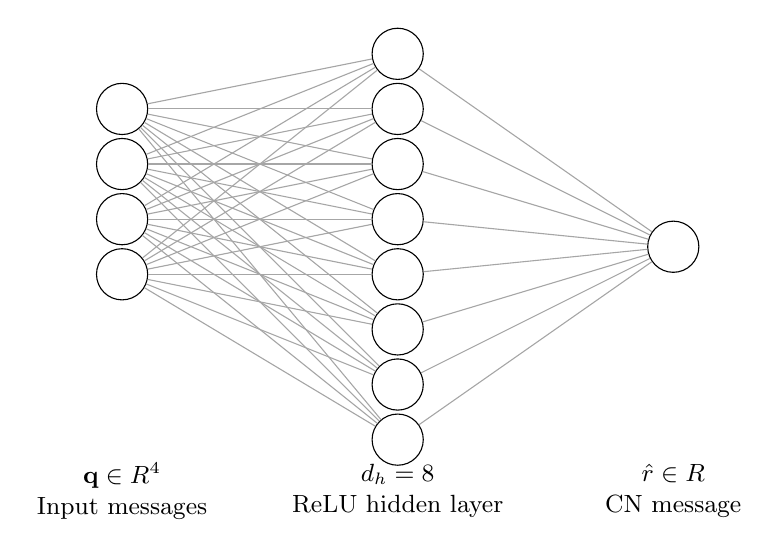
\begin{tikzpicture}[
  neuron/.style={circle,draw,minimum size=6.5mm,inner sep=0pt},
  conn/.style={thin,gray!70},
  font=\small
]
\foreach \i in {1,...,4}
  \node[neuron] (in\i) at (0,2.1-0.7*\i) {};
\foreach \i in {1,...,8}
  \node[neuron] (h\i) at (3.5,2.8-0.7*\i) {};
\node[neuron] (out) at (7,-0.35) {};
\foreach \i in {1,...,4}
  \foreach \j in {1,...,8}
    \draw[conn] (in\i) -- (h\j);
\foreach \j in {1,...,8}
  \draw[conn] (h\j) -- (out);
\node[align=center] at (0,-3.45) {$\mathbf{q}\in\mathbb{R}^{4}$\\Input messages};
\node[align=center] at (3.5,-3.45) {$d_h=8$\\ReLU hidden layer};
\node[align=center] at (7,-3.45) {$\hat{r}\in\mathbb{R}$\\CN message};
\end{tikzpicture}
\caption{MLP nhỏ gọn gần đúng với bản cập nhật nút kiểm tra LDPC.}
\label{fig:ann_ldpc_mlp}
\end{figure}

Kiến trúc nhỏ gọn này có liên quan. Một bộ giải mã thần kinh lớn có thể cải thiện đường cong mô phỏng nhưng sẽ khó chứng minh được bằng phần cứng. Một MLP nhỏ gọn có thể được đánh giá là sự thay thế cục bộ cho hàm phi tuyến. Nó có thể được tái sử dụng trên nhiều nút kiểm tra với cùng mức độ và có thể được lượng tử hóa hoặc định tuyến để triển khai phần cứng hiệu quả.

Hàm kích hoạt được sử dụng trong lớp ẩn là ReLU. Điều này đơn giản hơn tanh/log và thường được sử dụng vì nó làm giảm các vấn đề về độ biến thiên trong quá trình huấn luyện. Về phần cứng, ReLU cũng đơn giản vì bản chất nó là sự so sánh với con số 0. Do đó, chi phí chính của MLP là các hoạt động cộng nhân, thay vì các đánh giá siêu việt phi tuyến tính.

\begin{equation}
\hat{\mathbf{r}}=f_{\theta}(\mathbf{q}).
\end{equation}
Phương trình (3.11) biểu thị MLP rút gọn được sử dụng để tính gần đúng bản cập nhật CN. Đối với cấu hình 49 tham số đại diện, vectơ đầu vào là bốn thông báo VN-to-CN đi vào nút kiểm tra cấp 5 không bao gồm cạnh đi:
\begin{equation*}
\mathbf{q}_{i,j}^{(t)}=
\big[L_{j_1\rightarrow i}^{(t)},L_{j_2\rightarrow i}^{(t)},L_{j_3\rightarrow i}^{(t)},L_{j_4\rightarrow i}^{(t)}\big]^T,\quad
\{j_1,\ldots,j_4\}=\mathcal{N}(i)\setminus j .
\end{equation*}
Đầu ra $\hat{r}$ là tin nhắn CN-to-VN được ước tính ANN. Vì ReLU đơn giản và mạng nhỏ nên phương pháp này thân thiện với phần cứng hơn so với bộ giải mã thần kinh lớn.

\begin{equation}
\mathrm{ReLU}(x)=\max(x,0).
\end{equation}
Phương trình (3.12) xác định kích hoạt ReLU. Nó đơn giản về mặt tính toán và tránh được các hàm siêu việt đắt tiền.

\begin{equation}
N_{\theta}=d_{\mathrm{in}}d_h+d_h+d_hd_{\mathrm{out}}+d_{\mathrm{out}}.
\end{equation}
Phương trình (3.13) ước tính số lượng tham số có thể huấn luyện trong MLP một lớp ẩn. Biểu thức này hữu ích khi thảo luận về độ phức tạp của phần cứng. Với $d_{\mathrm{in}}=4$, $d_h=8$ và $d_{\mathrm{out}}=1$, số lượng tham số là
\begin{equation*}
N_{\theta}=4\times 8+8+8\times 1+1=49.
\end{equation*}
Nếu nút kiểm tra có cấp độ khác, bộ giải mã phải sử dụng mạng theo cấp độ cụ thể, chọn một tập hợp các tính năng tin cậy cố định, chẳng hạn như cường độ nhỏ nhất với sản phẩm ký hiệu được xử lý riêng hoặc đệm/cắt bớt đầu vào theo quy tắc triển khai đã nêu. Do đó, số lượng 49 tham số nên được hiểu là cấu hình nhỏ gọn đại diện được đánh giá trong luận án này chứ không phải là số lượng chung cho tất cả các ma trận LDPC.

\section{Chiến lược ghi nhãn và dữ liệu đào tạo}
Dữ liệu đào tạo được tạo ngoại tuyến bằng cách truyền BPSK qua kênh AWGN và mã QC-LDPC với các tham số $n=664$, $k=332$ và tốc độ $R_c=0.5$. Các khung ngẫu nhiên được mã hóa, truyền đi và chuyển đổi thành giá trị LLR. Các giá trị này được sử dụng để tính toán các thông báo cập nhật CN mục tiêu. Mạng được đào tạo với mất MAE, trình tối ưu hóa Adam, tốc độ học tập $10^{-3}$, kích thước lô 128 và 30 kỷ nguyên.

\begin{table}[H]
\centering
\caption{Thiết lập mô phỏng và đào tạo để giải mã LDPC được ANN hỗ trợ.}
\label{tab:ann_ldpc_config}
\begin{tabularx}{\textwidth}{p{0.33\textwidth}Y}
\toprule
Mục & Cấu hình được sử dụng trong kịch bản bộ giải mã được đánh giá\\
\midrule
Mã LDPC & QC-LDPC, $n=664$, $k=332$, $R_c=0.5$\\
Điều chế/kênh & BPSK qua AWGN để cách ly cập nhật nút kiểm tra LDPC\\
So sánh các bộ giải mã & SPA, Min-Sum, mô phỏng ANN-SPA và bản cập nhật ANN nhận biết độ tin cậy\\
Cài đặt lặp lại & Giao thức lặp lại tối đa cố định giống nhau cho tất cả các bộ giải mã được vẽ đồ thị; $I_{\max}$ chính xác và cờ dừng hội chứng phải được ghi lại bằng gói mô phỏng cuối cùng để có khả năng tái tạo đầy đủ\\
Mô hình ANN & MLP một lớp, $d_{\mathrm{in}}=4$, $d_h=8$, $d_{\mathrm{out}}=1$, Kích hoạt ẩn ReLU, 49 tham số có thể huấn luyện\\
Đào tạo & Mất MAE, trình tối ưu hóa Adam, tốc độ học tập $10^{-3}$, kích thước lô 128, 30 kỷ nguyên\\
Phạm vi đánh giá & SNR điểm từ $-1$ đến $7$ dB trong Hình~\ref{fig:ann_ldpc_ber_comparison}; đường cong được sử dụng làm bằng chứng ở mức xu hướng vì các xác nhận BER thấp ở mức tiêu chuẩn yêu cầu số khung, số bit và ghi nhật ký lỗi tối thiểu rõ ràng cho mỗi điểm SNR\\
\bottomrule
\end{tabularx}
\end{table}

\noindent\textbf{Reproducibility note.} The available ANN-LDPC material identifies the code length, rate, channel model, neural-network size, optimizer, learning rate, batch size, and training epochs. For a final archival simulation record, the following items should also be reported explicitly: the parity-check or base matrix used for the QC-LDPC code, the maximum iteration count $I_{\max}$, whether syndrome-based early stopping is enabled, the training/validation/test SNR split, the random seed or seed policy, and the transmitted-frame, transmitted-bit, and observed-error counts for each SNR point. Because these details cannot be inferred reliably from a BER figure alone, low-BER points in Figure~\ref{fig:ann_ldpc_ber_comparison} are interpreted as trend-level evidence rather than as standard-grade statistical claims.

\begin{figure}[H]
\centering

\includegraphics[width=0.78\textwidth]{ann_ldpc_training_loss.png}
\caption{Mất đào tạo mô hình nút kiểm tra ANN nhỏ gọn.}
\label{fig:ann_ldpc_training_loss}
\end{figure}

Hai kịch bản nhãn được xem xét. Trong kịch bản đầu tiên, ANN học cách ước chừng bản cập nhật SPA tiêu chuẩn. Mục đích là để tái tạo hành vi toán học của SPA mà không cần tính toán các hàm phi tuyến đắt tiền của nó trong quá trình suy luận. Kịch bản này xác nhận xem MLP có đủ khả năng để tìm hiểu quy tắc cập nhật cục bộ hay không.

Trong kịch bản thứ hai, các nhãn được sửa đổi bằng thông tin về độ tin cậy. Nếu dấu hiệu của thông báo SPA ồn ào không đồng ý với thông báo tham chiếu thì cường độ nhãn sẽ giảm. Điều này dạy cho mạng không tin tưởng vào một tin nhắn có vẻ không đáng tin cậy. Ý tưởng này có liên quan chặt chẽ đến khả năng giảm chấn và kiểm soát độ tin cậy, nhưng nó được học từ dữ liệu thay vì điều chỉnh thủ công.

\begin{equation}
\mathcal{L}_{\mathrm{MAE}}=\frac{1}{N}\sum_{n=1}^{N}\left|\hat{r}_n-r_n\right|.
\end{equation}
Phương trình (3.14) là tổn thất MAE được sử dụng cho việc huấn luyện. $r_n$ mục tiêu có thể là thông báo SPA hoặc nhãn nhận biết độ tin cậy nâng cao. MAE phù hợp vì mục tiêu là xấp xỉ các giá trị thông điệp hơn là phân loại trực tiếp các từ mã.

\begin{equation}
r_n=\begin{cases}r_n^{\mathrm{SPA}},&\mathrm{SPA\ label},\\ \eta_n r_n^{\mathrm{SPA}},&\mathrm{reliability\ aware\ label}.\end{cases}
\end{equation}
Phương trình (3.15) tóm tắt hai chiến lược gắn nhãn. Trường hợp đầu tiên huấn luyện ANN bắt chước SPA. Trong trường hợp thứ hai, $\eta_n\in[0,1]$ là hệ số độ tin cậy được chọn trong quá trình xây dựng nhãn ngoại tuyến. Thông báo tham chiếu được sử dụng để quyết định xem thông báo SPA ứng viên có đáng ngờ hay không không phải là đầu vào trực tuyến bổ sung cho ANN đã triển khai; mô hình đã triển khai chỉ nhận được vectơ cục bộ $\mathbf{q}$ và tạo ra bản cập nhật CN-to-VN. Nếu tham chiếu được tạo bằng cách sử dụng các bit được truyền sạch hoặc thông tin khác không có sẵn ở máy thu thực thì nhãn phải được hiểu là mục tiêu khả thi được thần đèn hỗ trợ để nghiên cứu độ suy giảm thông báo chứ không phải là đầu vào bộ giải mã có thể triển khai. Theo cách giải thích này, trường hợp thứ hai làm giảm cường độ của các thông báo không đáng tin cậy và cho phép ANN tìm hiểu hành vi giống như giảm xóc có thể làm giảm khuếch đại lỗi chu kỳ ngắn.

\begin{equation}
\theta^{\star}=\arg\min_{\theta}\mathbb{E}_{\mathbf{q},\mathbf{r}}\left[\ell(f_{\theta}(\mathbf{q}),\mathbf{r})\right].
\end{equation}
Phương trình (3.16) phát biểu bài toán huấn luyện ở dạng kỳ vọng. Hàm thần kinh $f_\theta$ được tối ưu hóa để gần đúng với bản cập nhật mục tiêu đã chọn.

\begin{equation}
\theta_{t+1}=\theta_t-\gamma_t\nabla_{\theta}\mathcal{L}(\theta_t).
\end{equation}
Phương trình (3.17) là cập nhật tham số chung dựa trên độ dốc. Trong quá trình triển khai, Adam được sử dụng thay vì giảm độ dốc đơn giản, nhưng phương trình giải thích nguyên tắc học tập.

\begin{equation}
\mathrm{SNR}_{\mathrm{dB}}=10\log_{10}\frac{E_s}{N_0}.
\end{equation}
Phương trình (3.18) biểu thị biến SNR được sử dụng khi tạo dữ liệu huấn luyện AWGN trên nhiều điều kiện kênh.

\section{Giải thích hai kịch bản}
Kịch bản gần đúng SPA là thận trọng. Nó yêu cầu ANN hoạt động giống như một thuật toán đã biết. Nếu đầu ra ANN gần với SPA và đường cong BER gần với SPA thì mô hình đã học thành công cập nhật phi tuyến. Giá trị của kịch bản này nằm ở việc giảm độ phức tạp và tính khả thi của phần cứng hơn là ở việc tạo ra nguyên tắc giải mã mới.

Kịch bản nhãn nâng cao có nhiều tham vọng hơn. Nó không chỉ đơn giản là bắt chước SPA. Nó sử dụng kiến ​​thức bổ sung để giảm mức độ nghiêm trọng của các thông báo bị nghi ngờ là sai. Điều này có liên quan vì việc giải mã lặp đi lặp lại có thể khuếch đại thông tin không chính xác. Một thông điệp sai có cường độ lớn có thể gây bất lợi hơn một thông điệp yếu kém vì nó có thể chi phối các quyết định sau này của VN.

Chu kỳ ngắn trong biểu đồ Tanner khiến vấn đề này trở nên nghiêm trọng hơn. Việc truyền bá niềm tin giả định rằng các tin nhắn đến gần như độc lập. Chu kỳ ngắn vi phạm giả định này vì thông tin có thể quay trở lại nút thông qua một đường dẫn ngắn. ANN không loại bỏ chu kỳ ngắn nhưng nó có thể học cách giảm các thông báo quá tự tin phát sinh từ thông tin tương quan.

\section{Thảo luận về hiệu suất}
So sánh BER trong Hình~\ref{fig:ann_ldpc_ber_comparison} cho thấy phép tính gần đúng ANN có thể đạt được hiệu suất BER gần bằng SPA và tốt hơn Min-Sum trong vùng thác nước của mã QC-LDPC được đánh giá. Đây là một kết quả phù hợp vì nó gợi ý rằng một mô hình thần kinh nhỏ gọn có thể duy trì hành vi chính của bản cập nhật CN phi tuyến. Kết quả hỗ trợ việc giải thích rằng mạng đang học ánh xạ toán học có cấu trúc thay vì liên kết đầu vào-đầu ra tùy ý.

\begin{figure}[H]
\centering

\includegraphics[width=0.86\textwidth]{ann_ldpc_ber_comparison.png}
\caption{So sánh BER cho các thuật toán giải mã QC-LDPC.}
\label{fig:ann_ldpc_ber_comparison}
\end{figure}

Trong kịch bản nhãn nâng cao, Hình~\ref{fig:ann_ldpc_ber_comparison} biểu thị mức tăng theo chiều ngang gần đúng theo thứ tự $0.2$--$0.4$ dB so với SPA xung quanh phần BER thấp của vùng thác nước, đặc biệt là gần thập kỷ $10^{-5}$ BER. Mức tăng này được đo theo mã QC-LDPC $(332,664)$ đã xác định, kênh BPSK/AWGN, quy trình đào tạo cố định và cài đặt lặp lại được đánh giá. Do số liệu kết quả hiện tại không bao gồm nhật ký số lỗi hoàn chỉnh trên mỗi SNR nên mức tăng phải được coi là kết quả ở mức xu hướng thay vì yêu cầu BER thấp ở mức tiêu chuẩn. Tuy nhiên, nó cung cấp bằng chứng cho thấy quy tắc cập nhật đã học đôi khi có thể hoạt động tốt hơn quy tắc SPA chính xác khi biểu đồ chứa các phụ thuộc thông báo bất lợi hoặc lợi ích từ cơ chế kiểm soát nhận biết độ tin cậy.

Đường cong huấn luyện-tổn thất hỗ trợ tính khả thi của mô hình. Sự mất mát giảm nhanh ở thời kỳ đầu và sau đó ổn định. Hành vi này chỉ ra rằng mạng tìm hiểu mối quan hệ phi tuyến chính mà không mất ổn định quá mức. Việc sử dụng nhiều giá trị SNR trong đào tạo cũng rất quan trọng vì nó làm giảm sự chuyên môn hóa quá mức xuống điều kiện độ tin cậy hẹp.

\begin{table}[H]
\centering
\caption{Hoạt động giải mã và giải thích cho nghiên cứu ANN-LDPC.}
\label{tab:ann_ldpc_decoder_comparison}
\begin{tabularx}{\textwidth}{p{0.23\textwidth}p{0.25\textwidth}Y}
\toprule
Bộ giải mã & Hoạt động chính & Giải thích trong luận văn này\\
\midrule
Cập nhật SPA & $\tanh(\cdot)$ và $\tanh^{-1}(\cdot)$ CN & Đường cơ sở hướng đến độ chính xác với chi phí vận hành phi tuyến tính cao\\
Tổng tối thiểu & Ký hiệu sản phẩm và cường độ tối thiểu & Đường cơ sở có độ phức tạp thấp với sự suy giảm BER có thể nhìn thấy trong Hình~\ref{fig:ann_ldpc_ber_comparison}\\
NMS/OMS & Hiệu chỉnh tỷ lệ hoặc bù cố định & Các tham chiếu tiêu chuẩn có độ phức tạp thấp được thảo luận về mặt phân tích; không được bao gồm dưới dạng đường cơ sở số được vẽ trong Hình~\ref{fig:ann_ldpc_ber_comparison} trừ khi đường cong được điều chỉnh riêng được cung cấp\\
Cập nhật ANN & Compact MLP với 49 tham số trong cài đặt đại diện & Xấp xỉ/hiệu chỉnh cục bộ của bản cập nhật CN; hữu ích khi mong muốn có hành vi giống như SPA mà không có chức năng siêu việt rõ ràng\\
\bottomrule
\end{tabularx}
\end{table}

\section{Quan điểm về độ phức tạp và phần cứng}
Ưu điểm phức tạp chính của phương pháp ANN là loại bỏ các phép toán tanh và logarit rõ ràng khỏi bản cập nhật nút kiểm tra SPA. Trong phần cứng, các hàm này thường yêu cầu bảng tra cứu, phép lặp CORDIC, xấp xỉ đa thức hoặc các đơn vị đặc biệt khác. Một MLP nhỏ gọn thay thế các hoạt động này bằng các phép tính cộng bội và kích hoạt ReLU, dễ dàng hơn trong việc xử lý và lượng tử hóa.

Kết quả phải được diễn giải thông qua cả BER và độ phức tạp của việc triển khai. Trong bộ giải mã LDPC thực tế, việc duy trì hiệu suất giống như SPA trong khi giảm chi phí tính toán nút kiểm tra phi tuyến đã có ý nghĩa. Do đó, phép tính gần đúng nút kiểm tra ANN cung cấp tùy chọn thiết kế theo hướng phức tạp, trong khi chiến lược nhãn nhận biết độ tin cậy có thể cung cấp cải thiện hiệu suất bổ sung trong các điều kiện đào tạo, kênh và biểu đồ đã chọn.

Sự so sánh công bằng phải bao gồm thông lượng, bộ nhớ, lượng tử hóa và khả năng tương thích lịch trình. Nếu trọng số ANN được chia sẻ trên các nút kiểm tra có cùng mức độ thì chi phí bộ nhớ sẽ vẫn nhỏ. Nếu mạng được lượng tử hóa, hệ số nhân có thể được đơn giản hóa. Nếu lịch trình LDPC ban đầu được giữ lại, phương pháp này có thể được đánh giá là sự thay thế cục bộ của chức năng nút kiểm tra thay vì là bộ giải mã thần kinh hoàn toàn.

Rủi ro kỹ thuật chính là khái quát hóa. Mạng được huấn luyện cho một cấp độ nút, một ma trận kiểm tra chẵn lẻ hoặc một định dạng lượng tử hóa có thể không chuyển trực tiếp sang cấu hình bộ giải mã khác. Đây là lý do tại sao luận án coi ANN là một phép tính gần đúng dựa trên mô hình mà giá trị của nó phải được đánh giá cùng với cấu trúc mã, phạm vi SNR và các ràng buộc triển khai.
\section{Ghi nhãn nhận biết độ tin cậy và giảm thiểu chu kỳ ngắn}
Chiến lược nhãn nâng cao trong giải mã LDPC được ANN hỗ trợ đáng được quan tâm đặc biệt vì nó không chỉ là một thủ thuật số. Trong học tập có giám sát thông thường, nhãn mục tiêu thường được coi là sự thật cơ bản. Tuy nhiên, ở đây bản thân thông báo SPA có thể không đáng tin cậy trong điều kiện nhiễu và các hiệu ứng chu kỳ ngắn. Do đó, quá trình đào tạo sử dụng nhãn đã điều chỉnh để hướng dẫn mạng về hành vi cập nhật thận trọng hơn.

Một chu kỳ ngắn trong biểu đồ Tanner khiến thông tin quay trở lại nút chỉ sau một vài bước truyền thông báo. Điều này vi phạm giả định độc lập đằng sau việc truyền bá niềm tin. Khi các thông điệp có mối tương quan với nhau, SPA có thể trở nên quá tự tin. Trong các bộ giải mã thực tế, sự giảm chấn đôi khi được sử dụng để giảm bớt vấn đề này. Phương pháp ANN được đề xuất có thể được hiểu là một cơ chế giảm chấn cục bộ đã học có độ mạnh phụ thuộc vào tính nhất quán của thông điệp~.

Dấu hiệu của thông báo LLR mang hướng quyết định cứng rắn, trong khi cường độ mang lại sự tin cậy. Một dấu sai có độ lớn nhỏ có thể được sửa ở những lần lặp sau. Một dấu hiệu sai với cường độ lớn có thể gây rắc rối hơn vì nó ngăn chặn những thông tin trái ngược nhau. Phương pháp nhãn nâng cao làm giảm mức độ của các thông báo đáng ngờ, có thể làm giảm sự hội tụ sớm hướng tới quyết định giải mã không chính xác.

Cơ chế này giải thích tại sao ANN nâng cao có thể cho thấy sự thay đổi thuận lợi so với SPA trong kịch bản có độ dài hữu hạn được đánh giá. SPA là tối ưu trên đồ thị không có chu trình theo các giả định xác suất chính xác, nhưng đồ thị LDPC hữu hạn chứa các chu trình. Nếu cấu trúc biểu đồ và việc thực hiện nhiễu tạo ra các thông báo sai lệch thì hành vi giảm chấn đã học có thể cải thiện hiệu suất thực tế. Điều này không mâu thuẫn với lý thuyết SPA; nó phản ánh sự khác biệt giữa các giả định lý tưởng và đồ thị vòng lặp hữu hạn.

Phương pháp này cũng có mối liên hệ với Tổng Min-Sum chuẩn hóa. Tổng tối thiểu được chuẩn hóa làm giảm cường độ thông báo bằng cách sử dụng hệ số cố định. ANN nâng cao có thể được xem dưới dạng chuẩn hóa phi tuyến tính và phụ thuộc vào dữ liệu. Thay vì áp dụng cùng một tỷ lệ ở mọi nơi, nó sẽ học khi nào một thông điệp cần được giữ nguyên và khi nào nó nên bị suy yếu. Đây là một dạng gần đúng linh hoạt hơn, nhưng nó đòi hỏi dữ liệu huấn luyện và xác nhận.

Đối với công việc trong tương lai, thiết kế nhãn nhận biết độ tin cậy có thể được mở rộng. Hệ số giảm có thể phụ thuộc vào SNR, chỉ số lặp, mức độ nút hoặc sự phân bố cường độ tới. Mạng cũng có thể xuất ra cả giá trị thông báo và ước tính độ tin cậy. Những phần mở rộng như vậy sẽ làm cho bộ giải mã ANN có khả năng thích ứng cao hơn, nhưng chúng cũng sẽ làm tăng độ phức tạp trong quá trình huấn luyện và yêu cầu các bài kiểm tra khái quát hóa cẩn thận.

Do đó, ANN nhãn nâng cao được coi là đóng góp có giới hạn. Nó giải quyết một hạn chế đã biết của việc truyền bá niềm tin điên rồ, trong khi mức tăng quan sát được vẫn phụ thuộc vào cấu trúc nhãn và sự giống nhau giữa điều kiện đào tạo và kiểm tra.

Một lợi thế kỹ thuật quan trọng là phương pháp này có thể được áp dụng tại địa phương. Lịch trình giải mã LDPC hiện tại có thể được giữ lại. Chỉ có chức năng cập nhật CN thay đổi. Điều này làm giảm rủi ro khi triển khai và giúp dễ dàng so sánh phương pháp được đề xuất với SPA, Min-Sum và Min-Sum chuẩn hóa trong các điều kiện mô phỏng giống hệt nhau.

\section{Từ SPA đến xấp xỉ nút kiểm tra thần kinh}
Phần LDPC của luận án mạnh nhất khi nó được hiểu là một phép tính gần đúng thần kinh dựa trên mô hình chứ không phải là một ứng dụng hộp đen chung chung của học sâu. Đồ thị Tanner đã cung cấp một cấu trúc tính toán chính xác. Mỗi nút biến đại diện cho một bit được mã hóa, mỗi nút kiểm tra đại diện cho một ràng buộc chẵn lẻ và mỗi cạnh mang một thông điệp mềm. Mạng nơ-ron chỉ được giới thiệu khi cập nhật nút kiểm tra, mạng này vừa phi tuyến vừa được đánh giá nhiều lần. Công thức cục bộ này rất quan trọng vì nó bảo toàn các ràng buộc mã LDPC và tránh thay thế toàn bộ bộ giải mã bằng một bộ phân loại mờ đục.

Để kiểm tra tính chẵn lẻ liên quan đến tập hợp các nút biến $\mathcal{N}(i)$, ràng buộc là
\begin{equation}
  \bigoplus_{j\in\mathcal{N}(i)} c_j=0.
\end{equation}
Trong quá trình truyền bá niềm tin, thông báo từ nút kiểm tra $i$ đến nút biến $j$ phụ thuộc vào tất cả các thông báo đến từ các nút biến khác được kết nối với cùng một kiểm tra:
\begin{equation}
  L_{i\rightarrow j}=F_{\mathrm{CN}}\left(\{L_{j'\rightarrow i}:j'\in\mathcal{N}(i)\setminus j\}\right).
\end{equation}
Hàm SPA chính xác trong miền LLR là
\begin{equation}
  F_{\mathrm{CN}}(\mathbf{q})=
  2\tanh^{-1}\left(\prod_{\ell}\tanh\frac{q_\ell}{2}\right).
\end{equation}
Hàm này có ý nghĩa xác suất rõ ràng. Nó kết hợp các dấu hiệu của tin nhắn đến để xác định tính nhất quán chẵn lẻ và kết hợp độ lớn của chúng để xác định độ tin cậy. Phần dấu hiệu rất đơn giản:
\begin{equation}
  \mathrm{sign}\left(F_{\mathrm{CN}}(\mathbf{q})\right)
  =
  \prod_{\ell}\mathrm{sign}(q_\ell).
\end{equation}
Phần khó khăn là độ lớn. Độ lớn phụ thuộc vào tất cả độ tin cậy đến thông qua các hàm hyperbol phi tuyến. Phép tính gần đúng Min-Sum chỉ giữ lại độ tin cậy yếu nhất:
\begin{equation}
  |F_{\mathrm{MS}}(\mathbf{q})|=\min_{\ell}|q_\ell|.
\end{equation}
Phép tính gần đúng này có hiệu quả về mặt tính toán nhưng đánh giá quá cao một cách có hệ thống cường độ SPA trong nhiều trường hợp. Tổng tối thiểu được chuẩn hóa và Tổng tối thiểu bù đắp điều chỉnh xu hướng này bằng cách áp dụng hệ số tỷ lệ hoặc độ lệch biên độ. Cách tiếp cận ANN khái quát hóa ý tưởng này. Thay vì sử dụng một quy tắc hiệu chỉnh cố định, mạng nơron học cách ánh xạ phi tuyến từ vectơ cường độ đầu vào đến cường độ đầu ra mục tiêu.

Bản cập nhật nút kiểm tra cũng có thể được viết thông qua toán tử box-plus:
\begin{equation}
  a\boxplus b
  =
  2\tanh^{-1}\left(\tanh\frac{a}{2}\tanh\frac{b}{2}\right).
\end{equation}
Sử dụng logarit Jacobian, phép toán này có dạng tương đương
\begin{equation}
  a\boxplus b
  =
  \mathrm{sign}(ab)\min(|a|,|b|)
  +\log\left(1+e^{-|a+b|}\right)
  -\log\left(1+e^{-|a-b|}\right).
\end{equation}
Thuật ngữ đầu tiên là phần Min-Sum. Hai số hạng logarit là hệ số hiệu chỉnh. Phương trình này giải thích tại sao Min-Sum hoạt động khá tốt và cũng tại sao nó không chính xác. Nó cũng cung cấp cách giải thích lý thuyết về mô hình thần kinh: MLP có thể được coi là học cách hiệu chỉnh phụ thuộc vào dữ liệu đối với cường độ Min-Sum mà không tính toán rõ ràng các thuật ngữ logarit.

Đối với nút kiểm tra cấp $d_c$, đầu vào ANN cho một cạnh đi có kích thước $d_c-1$. Nếu bộ giải mã sử dụng các tin nhắn đến thô
\begin{equation}
  \mathbf{q}_{i,j}^{(t)}
  =
  [L_{j_1\rightarrow i}^{(t)},\ldots,L_{j_{d_c-1}\rightarrow i}^{(t)}]^T,
\end{equation}
thì xấp xỉ thần kinh là
\begin{equation}
  \hat{L}_{i\rightarrow j}^{(t)}
  =
  f_\theta(\mathbf{q}_{i,j}^{(t)}).
\end{equation}
Đối với cấu hình 49 tham số nhỏ gọn được nhấn mạnh trong thử nghiệm bộ giải mã được báo cáo, điều này tương ứng với bản cập nhật cục bộ cấp 5, do đó $d_c-1=4$ và $\mathbf{q}_{i,j}^{(t)}\in\mathbb{R}^4$. Do đó, mô hình này không nên được mô tả như một sự thay thế có kích thước cố định phổ quát cho các nút kiểm tra LDPC tùy ý. Đối với các mức độ khác, việc triển khai phải đào tạo các mạng theo mức độ cụ thể, sử dụng quy tắc chọn tính năng hoặc phần đệm được xác định rõ ràng hoặc áp dụng kiến ​​trúc bất biến hoán vị.
Tuy nhiên, chức năng nút kiểm tra có tính đối xứng hữu ích. Dấu đầu ra được xác định bằng tích của các dấu đầu vào, trong khi cường độ được xác định bởi cường độ đầu vào. Do đó, việc triển khai có cấu trúc hơn có thể tính toán
\begin{equation}
  \hat{L}_{i\rightarrow j}^{(t)}
  =
  \left(\prod_{\ell}\mathrm{sign}(q_\ell)\right)
  g_\theta(|q_1|,\ldots,|q_{d_c-1}|).
\end{equation}
Cấu trúc này làm giảm gánh nặng cho mạng nơ-ron vì mạng không cần học tính đối xứng dấu hiệu từ dữ liệu. Nó chỉ học cách điều chỉnh cường độ. Ngay cả khi MLP nhỏ gọn được sử dụng trực tiếp cho chức năng cập nhật, việc diễn giải dựa trên tính đối xứng này rất quan trọng đối với việc sàng lọc thiết kế theo định hướng phần cứng sau này.

\section{Dữ liệu đào tạo, thiết kế nhãn và logic xác thực}
Chất lượng của bộ giải mã được hỗ trợ ANN phụ thuộc rất nhiều vào cách xây dựng nhãn huấn luyện. Trong kịch bản gần đúng SPA, nhãn mục tiêu là đầu ra nút kiểm tra SPA chính xác hoặc có độ chính xác cao:
\begin{equation}
  r^{\mathrm{target}}=F_{\mathrm{SPA}}(\mathbf{q}).
\end{equation}
Kịch bản này kiểm tra xem MLP có thể học hàm phi tuyến xác định hay không. Nếu mạng gần đúng với SPA trên phạm vi tin nhắn được sử dụng trong quá trình giải mã thì BER dự kiến ​​sẽ gần với SPA. Lợi ích sau đó là giảm độ phức tạp, đặc biệt nếu hàm thần kinh dễ lượng tử hóa hoặc đường dẫn hơn so với hàm phi tuyến ban đầu.

Trong kịch bản nhận biết độ tin cậy, mục tiêu được sửa đổi:
\begin{equation}
  r^{\mathrm{target}}=\rho(\mathbf{q},s,\mathrm{SNR})F_{\mathrm{SPA}}(\mathbf{q}),
\end{equation}
trong đó $\rho$ là hệ số tin cậy. Ở dạng đơn giản, $\rho<1$ khi tin nhắn bị nghi ngờ là không đáng tin cậy và $\rho\approx 1$ khi ngược lại. Chiến lược này liên quan đến quy tắc giảm xóc sau:
\begin{equation}
  L^{(t)}_{\mathrm{damped}}
  =
  \delta L^{(t)}+(1-\delta)L^{(t-1)},
\end{equation}
nhưng nó linh hoạt hơn vì độ suy giảm có thể phụ thuộc vào mẫu thông báo cục bộ hơn là vào một đại lượng vô hướng toàn cục cố định.

Thiết kế nhãn phải được xử lý cẩn thận. Nếu nhãn nhận biết độ tin cậy được tạo bằng cách sử dụng thông tin không có sẵn trong bộ giải mã thực, thì mô hình được đào tạo có thể ngầm học từ một nhà tiên tri không thực tế. Điều này không làm mất hiệu lực nghiên cứu nhưng nó làm thay đổi cách giải thích. Kết quả phải được mô tả là bằng chứng cho thấy việc kiểm soát cường độ thông điệp có thể cải thiện việc giải mã vòng lặp có độ dài hữu hạn trong các điều kiện đã chọn, chứ không phải là sự đảm bảo chung về tính ưu việt so với SPA. Đây là lý do tại sao luận án sử dụng ngôn ngữ hạn chế khi thảo luận về mức tăng xu hướng dB $0.2$--$0.4$ dB gần đúng được quan sát thấy trong Hình~\ref{fig:ann_ldpc_ber_comparison}.

Sự khác biệt tương tự cũng áp dụng cho các thông điệp tham chiếu được sử dụng trong quá trình xây dựng nhãn. Thông báo tham chiếu có thể được tạo ngoại tuyến từ tính toán SPA sạch hơn, từ mã được truyền đã biết hoặc quy tắc giáo viên khác. Những thông tin như vậy chỉ được sử dụng để xây dựng mục tiêu đào tạo. Trong quá trình suy luận, ANN đã triển khai nhận được vectơ tin nhắn đến cục bộ $\mathbf{q}_{i,j}^{(t)}$ và không nhận được các bit được truyền, tin nhắn kênh sạch hoặc cờ oracle rõ ràng. Nếu công trình mục tiêu sử dụng thông tin không có sẵn trên mạng thì kết quả sẽ được hiểu là nghiên cứu khả thi về khả năng giảm chấn đã học và kiểm soát độ tin cậy.

Một quy trình xác nhận mạnh mẽ sẽ tách biệt các phạm vi SNR đào tạo, xác nhận và kiểm tra. Nếu việc huấn luyện chỉ sử dụng một SNR thì mạng có thể học cách phân phối thông điệp hẹp. Ví dụ, ở mức SNR cao, hầu hết cường độ LLR đều lớn và dấu hiệu đáng tin cậy; ở cường độ SNR thấp là nhỏ và lỗi dấu xảy ra thường xuyên. Hiệu chỉnh thần kinh chỉ được huấn luyện ở SNR cao có thể vượt quá mức độ tin cậy của các tin nhắn ở SNR thấp. Việc điều chỉnh thần kinh chỉ được huấn luyện ở SNR thấp có thể làm giảm các thông điệp ở SNR cao một cách không cần thiết. Do đó, việc huấn luyện trên một phạm vi giá trị SNR phù hợp hơn với bộ giải mã được thiết kế để hoạt động trên các điều kiện kênh.

Đặt $\mathcal{S}_{\mathrm{train}}$ là tập hợp các giá trị SNR được sử dụng trong huấn luyện và $\mathcal{S}_{\mathrm{test}}$ là tập hợp được sử dụng trong thử nghiệm. Đánh giá mang tính thông tin nhất bao gồm cả phép nội suy và phép ngoại suy:
\begin{equation}
  \mathcal{S}_{\mathrm{test}}
  =
  \mathcal{S}_{\mathrm{interp}}\cup\mathcal{S}_{\mathrm{extra}},
\end{equation}
trong đó $\mathcal{S}_{\mathrm{interp}}$ nằm trong phạm vi huấn luyện và $\mathcal{S}_{\mathrm{extra}}$ nằm ngoài phạm vi huấn luyện. Một mô hình chỉ hoạt động ở dạng nội suy vẫn có thể hữu ích nhưng phạm vi hoạt động phải được nêu rõ ràng.

Hàm mất mát cũng ảnh hưởng đến hành vi đã học. MAE phạt lỗi tin nhắn tuyệt đối:
\begin{equation}
  \mathcal{L}_{\mathrm{MAE}}=\frac{1}{N}\sum_{n=1}^{N}|\hat{r}_n-r_n|.
\end{equation}
Sai số bình phương trung bình sẽ xử phạt các lỗi lớn mạnh hơn:
\begin{equation}
  \mathcal{L}_{\mathrm{MSE}}=\frac{1}{N}\sum_{n=1}^{N}(\hat{r}_n-r_n)^2.
\end{equation}
Đối với các bản tin LLR, tổn thất tốt nhất không phải lúc nào cũng rõ ràng. Một sai số tuyệt đối nhỏ gần bằng 0 có thể làm thay đổi dấu quyết định cứng và có thể gây hại nhiều hơn một sai số có độ lớn lớn hơn khi dấu đã đáng tin cậy. Việc mất mát do nhận biết được dấu hiệu có thể bao gồm một hình phạt bổ sung:
\begin{equation}
  \mathcal{L}_{\mathrm{sign}}
  =
  \mathcal{L}_{\mathrm{MAE}}
  +
  \lambda
  \frac{1}{N}\sum_{n=1}^{N}
  \mathbf{1}\{\mathrm{sign}(\hat{r}_n)\ne\mathrm{sign}(r_n)\}.
\end{equation}
Luận án này không yêu cầu sự mất mát như vậy để biện minh cho kết quả hiện tại, nhưng việc thảo luận về nó sẽ làm rõ mối liên hệ giữa độ chính xác hồi quy và hiệu suất giải mã~.

\section{Tính toán độ phức tạp cho giải mã LDPC được ANN hỗ trợ}
Đánh giá độ phức tạp chính xác đòi hỏi nhiều hơn tuyên bố rằng mạng lưới thần kinh nhỏ. Số lượng tham số là một phần của đối số, nhưng số lượng thao tác trên mỗi lần lặp và kiểu truy cập bộ nhớ cũng rất quan trọng. Hãy xem xét MLP một lớp ẩn với kích thước đầu vào $d_{\mathrm{in}}$, kích thước ẩn $d_h$ và kích thước đầu ra $d_{\mathrm{out}}=1$. Số lượng trọng số và độ lệch là
\begin{equation}
  N_\theta=d_{\mathrm{in}}d_h+d_h+d_h d_{\mathrm{out}}+d_{\mathrm{out}},
\end{equation}
trong đó hai thuật ngữ đầu tiên thuộc về lớp ẩn và hai thuật ngữ cuối cùng thuộc về lớp đầu ra. Số lượng phép toán tích lũy nhân trên mỗi suy luận là xấp xỉ
\begin{equation}
  C_{\mathrm{MLP}}\approx d_{\mathrm{in}}d_h+d_h d_{\mathrm{out}}.
\end{equation}
Đối với cấu hình 49 tham số đại diện được sử dụng trong luận án này, $d_{\mathrm{in}}=4$, $d_h=8$ và $d_{\mathrm{out}}=1$. Do đó, chi phí suy luận là khoảng $4\times 8+8\times 1=40$ hoạt động tích lũy nhân trên mỗi tin nhắn gửi đi, cộng với so sánh ReLU. Việc này có rẻ hơn SPA hay không phụ thuộc vào chi phí phần cứng được gán cho việc truy cập tanh, tanh nghịch đảo hoặc bảng tra cứu. Trong phần cứng kỹ thuật số, phép cộng nhân có thể rẻ hơn và dễ thực hiện hơn phép toán siêu việt có độ chính xác cao, đặc biệt khi trọng lượng được lượng tử hóa.

Nếu đồ thị Tanner có các cạnh $E$ và bộ giải mã chạy các vòng lặp $I_{\max}$, thì bản cập nhật nút kiểm tra cục bộ được đánh giá theo thứ tự $E I_{\max}$ lần. Do đó, tổng số hoạt động ANN là khoảng
\begin{equation}
  C_{\mathrm{total}}\approx E I_{\max} C_{\mathrm{MLP}}.
\end{equation}
Biểu thức này cho thấy tại sao mạng phải luôn nhỏ gọn. Một mạng lưới thần kinh lớn có thể chấp nhận được đối với một lần cập nhật nút kiểm tra, nhưng chi phí sẽ được nhân lên bởi tất cả các cạnh và tất cả các lần lặp. Do đó, kiến ​​trúc MLP cục bộ là một thiết kế có tính bảo vệ cao hơn một bộ giải mã đầu cuối lớn.

Chi phí bộ nhớ cũng có vấn đề. Nếu một tập hợp trọng số được chia sẻ trên tất cả các nút kiểm tra có cùng mức độ thì bộ nhớ tham số sẽ nhỏ:
\begin{equation}
  M_{\theta}=N_{\theta}Q_w,
\end{equation}
trong đó $Q_w$ là số bit trên mỗi trọng lượng. Với lượng tử hóa 8 bit và 49 tham số, bộ nhớ trọng lượng chỉ vài trăm bit. Nếu các trọng số riêng biệt được học cho mỗi nút hoặc mỗi lần lặp thì chi phí bộ nhớ sẽ tăng đáng kể. Do đó, luận án ủng hộ việc chia sẻ trọng số và cấu trúc hướng mô hình vì chúng phù hợp với bộ thu thực tế.

Lượng tử hóa có thể được tích hợp vào mô hình thần kinh. Mạng điểm cố định tính toán
\begin{equation}
  \hat{r}=Q_o\left(f_{Q_\theta(\theta)}(Q_i(\mathbf{q}))\right),
\end{equation}
trong đó $Q_i$, $Q_\theta$ và $Q_o$ là các bộ lượng tử hóa cho thông báo đầu vào, trọng số và thông báo đầu ra. Đào tạo nhận biết lượng tử hóa có thể mô phỏng các bộ lượng tử hóa này trong quá trình đào tạo để mạng học các tham số mạnh mẽ đến độ chính xác hữu hạn. Đây sẽ là sự tiếp nối quan trọng của công việc hiện tại vì bộ giải mã LDPC thường được triển khai với các thông báo điểm cố định.

\section{Giải thích khoa học về lợi ích quan sát được}
Mức tăng của kịch bản ANN nâng cao phải được trình bày dưới dạng kết quả có điều kiện. Trong nghiên cứu truyền thông, cải tiến BER chỉ có ý nghĩa khi biết mã, độ dài khối, điều chế, mô hình kênh, lịch trình giải mã, số lần lặp và độ dài mô phỏng. Không thể khái quát đường cong thu được cho một mã QC-LDPC trên AWGN cho tất cả các mã LDPC hoặc tất cả cấu hình BIBCM-ID. Do đó, luận án giải thích mức tăng là bằng chứng cho thấy điều khiển độ tin cậy đã học có thể cải thiện bộ giải mã vòng lặp có độ dài hữu hạn cụ thể.

Cách giải thích này mạnh mẽ hơn về mặt khoa học so với một tuyên bố phóng đại. SPA là tối ưu cho các biểu đồ nhân tố dạng cây theo mô hình xác suất chính xác, nhưng biểu đồ LDPC thực tế chứa các chu trình. Trong biểu đồ lặp, các thông điệp có thể trở nên tương quan. Khi các thông điệp tương quan được kết hợp nhiều lần, bộ giải mã có thể trở nên quá tự tin. Sự suy giảm nhận biết độ tin cậy có thể làm giảm hiệu ứng này. Do đó, phương pháp ANN không mâu thuẫn với lý thuyết về SPA; nó đang khai thác sự khác biệt giữa các giả định lý tưởng đằng sau SPA và các điều kiện có độ dài hữu hạn của việc giải mã thực tế.

Kết quả phía bộ giải mã cũng liên quan đến BIBCM-ID vì khối Giải điều chế có thể cung cấp LLR không hoàn hảo. Nếu đầu ra Giải điều chế hơi sai lệch hoặc quá tự tin, bản cập nhật LDPC nhận biết độ tin cậy có thể ngăn bộ giải mã khuếch đại độ lệch đó quá nhanh. Đây là một lợi ích hợp lý ở cấp độ hệ thống ngay cả trước khi xem xét việc tối ưu hóa chung Điều chế và giải mã. Do đó, bộ giải mã ANN được coi là một sửa đổi có kiểm soát bên trong bộ giải mã kênh, trong khi Điều chế bộ mã hóa tự động được coi là một cuộc điều tra bổ sung về nguồn thông tin mềm.

Lợi ích phức tạp phụ thuộc vào đường cơ sở thực hiện. So với Min-Sum, ANN có thể phức tạp hơn. So với SPA chính xác sử dụng tanh và nghịch đảo tanh, ANN có thể thân thiện với phần cứng hơn. Do đó, tuyên bố công bằng không phải là ANN luôn là bộ giải mã có độ phức tạp thấp nhất mà nó mang lại sự cân bằng giữa hiệu suất giống như SPA và phép tính gần đúng phi tuyến có thể thực hiện được.

Khái quát hóa vẫn là một yêu cầu kỹ thuật và có thể được kiểm tra thông qua nhiều ma trận kiểm tra chẵn lẻ, nhiều cấp độ nút, nhiều phạm vi SNR, thông báo lượng tử hóa và các điều kiện kênh không khớp. Điều này không làm suy yếu sự đóng góp hiện tại; nó đặt nó ở mức độ bằng chứng chính xác. Nghiên cứu này trình bày một phương pháp tập trung và diễn giải nó với các ranh giới kỹ thuật~ thích hợp.

\section{Giao thức đánh giá cho giải mã được hỗ trợ bởi ANN}
Nghiên cứu bộ giải mã thuyết phục về mặt kỹ thuật đòi hỏi một giao thức đánh giá tách biệt hiệu ứng thuật toán khỏi tạo phẩm mô phỏng. Đường cong BER là kết quả dễ thấy nhất nhưng nó không phải là bằng chứng duy nhất. Để so sánh công bằng, các thuật toán cơ sở phải sử dụng cùng mã, điều chế, mô hình kênh, giới hạn lặp, quy tắc dừng và chia tỷ lệ LLR. Nếu bất kỳ điều kiện nào trong số này khác nhau thì việc so sánh có thể phản ánh sự khác biệt trong việc triển khai hơn là lợi thế giải mã thực sự.

Yêu cầu đầu tiên là cấu hình mã nhất quán. Đối với mã LDPC có độ dài khối $n$, độ dài thông tin $k$ và tốc độ $R_c=k/n$, mọi bộ giải mã so sánh phải hoạt động trên cùng một ma trận kiểm tra chẵn lẻ $\mathbf{H}$. Nếu ANN được huấn luyện cho ma trận QC-LDPC, bài kiểm tra phải nêu rõ liệu ma trận tương tự được sử dụng hay ma trận khác được sử dụng để khái quát hóa. Bộ giải mã hoạt động tốt trên một ma trận có cấu trúc có thể không tự động chuyển sang ma trận khác do sự phân bố cấp độ nút, chu kỳ ngắn và bộ bẫy thay đổi.

Yêu cầu thứ hai là cài đặt kênh và điều chế nhất quán. Nếu dữ liệu huấn luyện được tạo từ BPSK qua AWGN thì lần xác thực đầu tiên sẽ sử dụng cài đặt tương tự để tách biệt phép tính gần đúng của nút kiểm tra. Chỉ sau đó, phương pháp này mới được thử nghiệm với Điều chế bậc cao hơn hoặc với đầu vào Giải điều chế mềm kiểu BIBCM-ID. Đánh giá theo giai đoạn này là quan trọng. Nó ngăn không cho một thử nghiệm kết hợp quá nhiều hiệu ứng: kênh không khớp, giải điều chế không khớp, hành vi đồ thị LDPC và lỗi xấp xỉ thần kinh.

Yêu cầu thứ ba là đủ số lượng bit mô phỏng. Ở mức BER thấp, một số lượng nhỏ sai số sẽ tạo ra ước tính nhiễu. Nếu quan sát thấy lỗi $N_{\mathrm{err}}$ trên các bit được truyền $N_{\mathrm{bit}}$ thì ước tính BER là
\begin{equation}
  \widehat{\mathrm{BER}}=\frac{N_{\mathrm{err}}}{N_{\mathrm{bit}}}.
\end{equation}
Đối với các lỗi hiếm gặp, độ không đảm bảo tương đối lớn khi $N_{\mathrm{err}}$ nhỏ. Một quy tắc đơn giản trong mô phỏng giao tiếp là thu thập số lượng sự kiện lỗi tối thiểu trước khi tin cậy một điểm trên đường cong BER. Do đó, điểm BER thấp dựa trên quá ít lỗi chỉ được hiểu là xu hướng biểu thị chứ không phải là bằng chứng mạnh mẽ về tính ưu việt.

Yêu cầu thứ tư là báo cáo giới hạn lặp và quy tắc dừng. Quy tắc dừng dựa trên hội chứng kết thúc việc giải mã khi
\begin{equation}
  \mathbf{H}\hat{\mathbf{c}}^T=\mathbf{0}.
\end{equation}
Đối với kết quả ANN-LDPC, so sánh được hiểu là đánh giá cùng một giao thức, nhưng tài liệu được trích xuất không cung cấp bản ghi $I_{\max}$, trạng thái quy tắc dừng và số lần lặp trung bình trên mỗi SNR hoàn chỉnh. Số lượng này phải được đưa vào kho lưu trữ mô phỏng cuối cùng trước khi đưa ra các tuyên bố mạnh mẽ ở cấp độ triển khai. Nếu một bộ giải mã đạt đến điều kiện hội chứng sớm hơn bộ giải mã khác, nó có thể giảm độ phức tạp trung bình ngay cả khi giới hạn lặp tối đa là như nhau. Do đó, số lần lặp trung bình là một thước đo đồng hành hữu ích:
\begin{equation}
  \bar{I}=\frac{1}{N_f}\sum_{r=1}^{N_f}I_r,
\end{equation}
trong đó $N_f$ là số khung mô phỏng và $I_r$ là số lần lặp được sử dụng cho khung $r$. Bộ giải mã bảo toàn BER trong khi giảm $\bar{I}$ có thể hấp dẫn ngay cả khi chi phí mỗi lần lặp của nó cao hơn một chút.

Yêu cầu thứ năm là bao gồm tỷ lệ lỗi khung khi có thể. BER đo tỷ lệ bit sai, trong khi FER đo xem toàn bộ khung có được giải mã chính xác hay không:
\begin{equation}
  \mathrm{FER}=\frac{N_{\mathrm{frame,err}}}{N_{\mathrm{frame}}}.
\end{equation}
Trong các hệ thống được mã hóa, FER thường rất quan trọng vì nhiều ứng dụng coi khung có một lỗi là không thể sử dụng được. Bản cập nhật nút kiểm tra ANN làm giảm BER nhưng giữ nguyên FER vẫn có thể hữu ích, nhưng cần hiểu rõ sự khác biệt.

\section{Chế độ xem Ablation của bộ giải mã ANN}
Chế độ xem cắt bỏ làm rõ phần nào của phương pháp chịu trách nhiệm về hành vi được quan sát. Sự cắt bỏ đầu tiên là bắt chước SPA so với ghi nhãn nhận biết độ tin cậy. Nếu mạng giả SPA khớp với SPA, điều này hỗ trợ cho tuyên bố rằng MLP có thể gần đúng với chức năng nút kiểm tra phi tuyến. Nếu mạng nhận biết độ tin cậy cải thiện đường cong, điều này hỗ trợ cho khẳng định bổ sung rằng việc kiểm soát cường độ đã học có thể có lợi khi giải mã vòng lặp hữu hạn. Hai tuyên bố này nên được đánh giá riêng biệt.

Sự cắt bỏ thứ hai là kích thước mạng. Một mạng nhỏ gọn là trung tâm của lập luận kỹ thuật. Nếu mạng lớn hơn cải thiện BER một chút nhưng chi phí lại tăng lên đáng kể thì nó có thể ít liên quan hơn đến việc triển khai máy thu. Do đó, kích thước lớp ẩn phải được hiểu là một biến thiết kế trong sự cân bằng giữa hiệu suất và độ phức tạp:
\begin{equation}
  \mathrm{Tradeoff}=
  \left(\mathrm{BER},\ \mathrm{FER},\ \bar{I},\ C_{\mathrm{op}},\ M_{\theta}\right),
\end{equation}
trong đó $C_{\mathrm{op}}$ biểu thị các hoạt động tính toán và $M_{\theta}$ biểu thị bộ nhớ mô hình. Chế độ xem vectơ này mang lại nhiều thông tin hơn một số BER đơn lẻ.

Sự cắt bỏ thứ ba là cắt tin nhắn. Bộ giải mã LDPC thường cắt LLR thành một phạm vi hữu hạn. Nếu ANN được huấn luyện trên các tin nhắn SPA dấu phẩy động chưa được cắt bớt nhưng được kiểm tra trong bộ giải mã được cắt bớt thì hiệu suất có thể thay đổi. Một bài kiểm tra công bằng nên huấn luyện và kiểm tra trong cùng một phạm vi cắt hoặc phân tích rõ ràng sự không khớp. Phạm vi cắt có thể được viết là
\begin{equation}
  L_{\mathrm{clip}}=\max(-L_{\max},\min(L,L_{\max})).
\end{equation}
Giá trị của $L_{\max}$ ảnh hưởng đến cả độ ổn định số và độ tin cậy giải mã.

Sự cắt bỏ thứ tư là mức độ nút. Một MLP duy nhất có thể được đào tạo cho một cấp độ nút kiểm tra. Nếu ma trận LDPC có nhiều cấp độ nút kiểm tra, bộ giải mã có thể sử dụng các mạng riêng biệt cho từng cấp độ, đệm đầu vào theo một chiều chung hoặc thiết kế kiến ​​trúc bất biến hoán vị. Mạng riêng biệt tăng bộ nhớ. Đệm có thể lãng phí tính toán. Một kiến ​​trúc bất biến hoán vị có thể được viết là
\begin{equation}
  g_\theta(\{|q_\ell|\})=
  \rho_\theta\left(\sum_{\ell}\psi_\theta(|q_\ell|)\right),
\end{equation}
trong đó $\psi_\theta$ và $\rho_\theta$ là các hàm có thể học được. Biểu mẫu này tôn trọng thực tế là việc cập nhật nút kiểm tra không nên phụ thuộc vào thứ tự tùy ý trong đó các thông báo được liệt kê.

Sự cắt bỏ thứ năm là sự phụ thuộc lặp lại. Mạng có thể chia sẻ các tham số giống nhau trên tất cả các lần lặp hoặc sử dụng các tham số dành riêng cho từng lần lặp. Các tham số được chia sẻ làm giảm bộ nhớ và dễ dàng điều chỉnh hơn. Các tham số dành riêng cho lần lặp có thể cải thiện hiệu suất nhưng có nguy cơ phù hợp quá mức với lịch trình lặp cố định. Đối với một bộ giải mã thực tế, sự phụ thuộc lặp được chia sẻ hoặc tham số hóa nhẹ là thích hợp hơn trừ khi mức tăng là đáng kể.

\section{Ranh giới khoa học của nghiên cứu bộ giải mã}
Việc so sánh giữa bộ giải mã ANN và Min-Sum chuẩn hóa phải được diễn giải thông qua cả tiêu chí hiệu suất và triển khai. Tổng tối thiểu được chuẩn hóa cực kỳ đơn giản và có thể thích hợp hơn khi độ phức tạp tối thiểu là mục tiêu duy nhất. Phương pháp ANN phù hợp hơn khi người thiết kế muốn hành vi giống như SPA mà không có chức năng siêu việt rõ ràng hoặc khi việc giảm chấn nhận biết độ tin cậy mang lại lợi thế được kiểm soát. Do đó, kết quả là một sự đánh đổi chứ không phải là một sự thay thế phổ biến.

Độ tin cậy thống kê của mức tăng BER phụ thuộc vào độ dài mô phỏng và số lượng lỗi quan sát được. Hình~\ref{fig:ann_ldpc_ber_comparison} cho thấy xu hướng thuận lợi trong các điều kiện QC-LDPC và BPSK/AWGN đã nêu, trong khi các yêu cầu ở mức tiêu chuẩn ở các vùng BER thấp hơn sẽ yêu cầu mô phỏng dài hơn và ghi nhật ký sự kiện lỗi rõ ràng tại mỗi điểm SNR. Cách giải thích này phù hợp với một nghiên cứu tập trung vào phân tích thuật toán và đánh giá tính khả thi.

Một bảng tái tạo hoàn chỉnh phải bao gồm, đối với mỗi điểm SNR, số khung được truyền, số bit thông tin được truyền, số lỗi bit quan sát được, số lỗi khung và kết quả dừng nếu kích hoạt tính năng kết thúc sớm. Nếu không có các trường này, đường cong BER vẫn hữu ích trong việc so sánh xu hướng giữa các thuật toán, nhưng phần đuôi BER thấp của nó sẽ không bị diễn giải quá mức.

ANN không loại bỏ khả năng diễn giải của giải mã LDPC vì phương pháp được đề xuất giữ nguyên biểu đồ Tanner và chỉ thay đổi chức năng cập nhật cục bộ. Ma trận kiểm tra chẵn lẻ, kiểm tra hội chứng, cập nhật nút biến và lịch trình lặp lại vẫn có thể hiểu được. MLP hoạt động như một phép tính gần đúng hoặc hiệu chỉnh đã học cho hoạt động của nút kiểm tra phi tuyến. Điều này rất khác với việc thay thế bộ giải mã bằng một bộ phân loại thần kinh ánh xạ trực tiếp các mẫu kênh tới các tin nhắn.

Phương pháp này tương thích với thông tin mềm từ Giải điều chế BIBCM-ID ở cấp độ giao diện thông báo: bộ giải mã LDPC sử dụng LLR bất kể chúng có nguồn gốc từ Giải điều chế BPSK hay Giải điều chế BIBCM-ID bậc cao. Tuy nhiên, việc phân phối các LLR đó có thể khác nhau. Do đó, BPSK-AWGN là đánh giá đầu tiên được kiểm soát, trong khi đầu vào mềm BIBCM-ID là bối cảnh hệ thống rộng hơn.

Những thách thức có thể xảy ra này không phải là khiếm khuyết nếu chúng được giải quyết một cách rõ ràng. Họ xác định ranh giới giữa sự đóng góp tập trung ở cấp độ thạc sĩ và việc triển khai bộ thu sẵn sàng theo tiêu chuẩn đầy đủ. Luận án sử dụng ranh giới này để giữ cho các tuyên bố trở nên đáng tin cậy: việc xử lý nút kiểm tra được ANN hỗ trợ là đóng góp chính; Điều chế AutoEncode là một phân tích hỗ trợ nguồn thông tin phần mềm; xác nhận đa kênh rộng hơn vẫn là một sự tiếp tục về mặt kỹ thuật.


\section{Kết luận chương}
Chương này đã phân tích giải mã LDPC với sự hỗ trợ của ANN là đóng góp kỹ thuật chính của luận án. Bắt đầu từ biểu diễn đồ thị Tanner và các phương trình truyền thông báo trong miền LLR, chương này đã xác định cập nhật nút kiểm tra là một phần đòi hỏi tính toán của quá trình giải mã SPA. Phép tính gần đúng Min-Sum làm giảm chi phí này nhưng mất đi một phần hiệu chỉnh phi tuyến có trong SPA. Sự cân bằng này thúc đẩy việc sử dụng mô hình thần kinh nhỏ gọn làm phép tính gần đúng cục bộ hoặc hiệu chỉnh hoạt động của nút kiểm tra.

Hướng thần kinh được đề xuất được điều khiển theo mô hình một cách có chủ ý. Ma trận kiểm tra chẵn lẻ, cập nhật nút biến, kiểm tra hội chứng và lịch trình giải mã lặp lại không thay đổi; chỉ cập nhật nút kiểm tra cục bộ là gần đúng hoặc được điều chỉnh. Trong cấu hình đại diện, MLP sử dụng bốn giá trị độ tin cậy đầu vào, tám đơn vị ẩn và một giá trị đầu ra, cung cấp 49 tham số có thể huấn luyện và khoảng 40 thao tác tích lũy nhân cho mỗi thông báo gửi đi. Thang đo nhỏ gọn này rất cần thiết cho khối giải mã được đánh giá nhiều lần trên tất cả các cạnh của đồ thị Tanner và các lần lặp giải mã.

Kết quả BER hỗ trợ hai kết luận với các mức độ khẳng định khác nhau. Đầu tiên, ANN được đào tạo để bắt chước SPA có thể duy trì hành vi giải mã gần với SPA trong khi tránh các phép tính tanh và nghịch đảo tanh rõ ràng. Kết quả này chủ yếu là một đóng góp theo định hướng phức tạp. Thứ hai, chiến lược nhãn nhận biết độ tin cậy cho thấy rằng sự suy giảm thông điệp đã học có thể cải thiện hành vi giải mã thực tế trong biểu đồ vòng lặp có độ dài hữu hạn được đánh giá. Độ lợi này được giải thích có điều kiện chứ không phải phổ quát, bởi vì nó phụ thuộc vào mã, mô hình kênh, nhãn huấn luyện, phạm vi SNR và độ dài mô phỏng. Do đó, chương này định vị việc giải mã LDPC được ANN hỗ trợ như một phương pháp kết hợp thực tế: nó giữ nguyên cấu trúc của lý thuyết mã hóa cổ điển trong khi sử dụng phương pháp học để ước chừng hoặc điều chỉnh cập nhật thông báo phi tuyến.

\chapter*{CONCLUSION AND RECOMMENDATIONS}
\addcontentsline{toc}{chapter}{\textbf{CONCLUSION AND RECOMMENDATIONS}}
Luận án này đã nghiên cứu ứng dụng mạng nơ-ron nhân tạo trong giải mã LDPC cho các hệ thống truyền thông định hướng BIBCM-ID. Phần lý thuyết đã xem xét vai trò của Điều chế, Giải điều chế, xen kẽ, thông tin mềm, giải mã kênh và học sâu theo hướng mô hình trong điều chế mã hóa lặp. Nền tảng này làm rõ lý do tại sao chất lượng của tin nhắn LLR là vấn đề trọng tâm: bộ giải mã LDPC hoạt động dựa trên thông tin đáng tin cậy và các tin nhắn không chính xác hoặc quá tự tin có thể làm giảm hiệu quả giải mã lặp lại.

\noindent\textbf{Validated decoder result.} The main technical contribution is the analysis of ANN-assisted LDPC decoding. A compact neural model is used to approximate the check-node update, which is one of the nonlinear and computationally expensive operations in SPA decoding. In the representative configuration, the MLP uses four input values, eight hidden units, one output value, and 49 trainable parameters; the corresponding inference cost is about 40 multiply-accumulate operations per outgoing message plus ReLU comparisons. For the QC-LDPC $(332,664)$ code over the BPSK/AWGN channel, Figure~\ref{fig:ann_ldpc_ber_comparison} shows that the ANN update follows the SPA curve closely and improves over Min-Sum in the waterfall region under the plotted conditions. In the enhanced-label case, the plotted curve indicates an approximate $0.2$--$0.4$ dB horizontal shift around the $10^{-5}$ BER decade. These results should be interpreted primarily in terms of complexity reduction, preservation of SPA-like decoding quality, and reliability-aware message control under the stated simulation conditions.

\noindent\textbf{Supporting system analysis.} The AutoEncoder Modulation study is included as a complementary analysis of the Modulation and Demodulation side of the BIBCM-ID soft-information chain. The simulation results in Chapter 2 show that learned signal representations can adapt to PA distortion, CFO, fading, and sequence-dependent channel effects. This part strengthens the discussion of how upstream signal mapping and receiver observation quality affect LDPC decoding, while the main quantitative evidence for the thesis remains the ANN-LDPC decoder analysis presented in Chapter 3.

\noindent\textbf{Recommendations.} Overall, the thesis supports a hybrid view of deep learning in communication systems. Neural networks are most defensible when they approximate difficult nonlinear operations, correct model mismatch, or improve the reliability of soft information while preserving the structure of established coding and modulation theory. Future work should focus on calibrated bit-level LLR output for neural Demodulation, broader validation over LDPC code structures and channel conditions, fixed-point and quantization-aware ANN decoder design, and complexity-throughput evaluation for practical receiver architectures. For the ANN-LDPC result specifically, a final simulation package should include the parity-check matrix, $I_{\max}$, stopping rule, random seeds, and per-SNR frame/error logs so that the reported BER trends can be reproduced and, where sufficient error counts are available, promoted to stronger statistical claims.
\begin{thebibliography}{99}
\addcontentsline{toc}{chapter}{\textbf{REFERENCES}}
\bibitem{bishop2006} C. M. Bishop, Pattern Recognition and Machine Learning. Springer, 2006.
\bibitem{lecun2015} Y. LeCun, Y. Bengio, and G. Hinton, ``Deep learning,'' Nature, vol. 521, pp. 436--444, 2015.
\bibitem{goodfellow2016} I. Goodfellow, Y. Bengio, and A. Courville, Deep Learning. MIT Press, 2016.
\bibitem{shannon1948} C. E. Shannon, ``A mathematical theory of communication,'' Bell System Technical Journal, vol. 27, no. 3, pp. 379--423, 1948.
\bibitem{gallager1962} R. G. Gallager, ``Low-density parity-check codes,'' IRE Transactions on Information Theory, vol. 8, no. 1, pp. 21--28, 1962.
\bibitem{tanner1981} R. M. Tanner, ``A recursive approach to low complexity codes,'' IEEE Transactions on Information Theory, vol. 27, no. 5, pp. 533--547, 1981.
\bibitem{mackay1996} D. J. C. MacKay and R. M. Neal, ``Near Shannon limit performance of low density parity check codes,'' Electronics Letters, vol. 32, no. 18, pp. 1645--1646, 1996.
\bibitem{kschischang2001} F. R. Kschischang, B. J. Frey, and H.-A. Loeliger, ``Factor graphs and the sum-product algorithm,'' IEEE Transactions on Information Theory, vol. 47, no. 2, pp. 498--519, 2001.
\bibitem{richardson2008} T. Richardson and R. Urbanke, Modern Coding Theory. Cambridge University Press, 2008.
\bibitem{hu2005peg} X.-Y. Hu, E. Eleftheriou, and D. M. Arnold, ``Regular and irregular progressive edge-growth Tanner graphs,'' IEEE Transactions on Information Theory, vol. 51, no. 1, pp. 386--398, 2005.
\bibitem{hu2001spa} X.-Y. Hu, E. Eleftheriou, D. M. Arnold, and A. Dholakia, ``Efficient implementations of the sum-product algorithm for decoding LDPC codes,'' in Proc. IEEE GLOBECOM, 2001.
\bibitem{chen2002} J. Chen and M. P. C. Fossorier, ``Near optimum universal belief propagation based decoding of low-density parity-check codes,'' IEEE Transactions on Communications, vol. 50, no. 3, pp. 406--414, 2002.
\bibitem{zarkeshvari2002} F. Zarkeshvari and A. H. Banihashemi, ``On implementation of min-sum algorithm for decoding low-density parity-check codes,'' in Proc. IEEE GLOBECOM, 2002.
\bibitem{zehavi1992} E. Zehavi, ``8-PSK trellis codes for a Rayleigh channel,'' IEEE Transactions on Communications, vol. 40, no. 5, pp. 873--884, 1992.
\bibitem{caire1998} G. Caire, G. Taricco, and E. Biglieri, ``Bit-interleaved coded modulation,'' IEEE Transactions on Information Theory, vol. 44, no. 3, pp. 927--946, 1998.
\bibitem{li1997} X. Li and J. A. Ritcey, ``Bit-interleaved coded modulation with iterative decoding,'' IEEE Communications Letters, vol. 1, no. 6, pp. 169--171, 1997.
\bibitem{li1998} X. Li, A. Chindapol, and J. A. Ritcey, ``Bit-interleaved coded modulation with iterative decoding and 8PSK signaling,'' IEEE Transactions on Communications, vol. 50, no. 8, pp. 1250--1257, 2002.
\bibitem{tenbrink2001} S. ten Brink, ``Convergence behavior of iteratively decoded parallel concatenated codes,'' IEEE Transactions on Communications, vol. 49, no. 10, pp. 1727--1737, 2001.
\bibitem{brink2004} S. ten Brink, G. Kramer, and A. Ashikhmin, ``Design of low-density parity-check codes for modulation and detection,'' IEEE Transactions on Communications, vol. 52, no. 4, pp. 670--678, 2004.
\bibitem{hagenauer1996} J. Hagenauer, E. Offer, and L. Papke, ``Iterative decoding of binary block and convolutional codes,'' IEEE Transactions on Information Theory, vol. 42, no. 2, pp. 429--445, 1996.
\bibitem{nachmani2016} E. Nachmani, Y. Be'ery, and D. Burshtein, ``Learning to decode linear codes using deep learning,'' in Proc. Allerton Conference on Communication, Control, and Computing, 2016.
\bibitem{nachmani2018} E. Nachmani, E. Marciano, L. Lugosch, W. J. Gross, D. Burshtein, and Y. Be'ery, ``Deep learning methods for improved decoding of linear codes,'' IEEE Journal of Selected Topics in Signal Processing, vol. 12, no. 1, pp. 119--131, 2018.
\bibitem{lugosch2017} L. Lugosch and W. J. Gross, ``Learning from the syndrome,'' in Proc. Asilomar Conference on Signals, Systems, and Computers, 2017.
\bibitem{kuck2020} J. Kuck, S. Han, and S. Mohan, ``Belief propagation neural networks,'' Advances in Neural Information Processing Systems, vol. 33, pp. 667--678, 2020.
\bibitem{wang2022} Q. Wang, S. ten Brink, and H. V. Poor, ``Normalized min-sum neural network for LDPC decoding,'' IEEE Transactions on Cognitive Communications and Networking, vol. 9, no. 1, pp. 70--81, 2023.
\bibitem{oshea2017} T. J. O'Shea and J. Hoydis, ``An introduction to deep learning for the physical layer,'' IEEE Transactions on Cognitive Communications and Networking, vol. 3, no. 4, pp. 563--575, 2017.
\bibitem{dorner2018} S. Dorner, S. Cammerer, J. Hoydis, and S. ten Brink, ``Deep learning based communication over the air,'' IEEE Journal of Selected Topics in Signal Processing, vol. 12, no. 1, pp. 132--143, 2018.
\bibitem{aoudia2019} F. A. Aoudia and J. Hoydis, ``End-to-end learning of communications systems without a channel model,'' in Proc. Asilomar Conference on Signals, Systems, and Computers, 2018.
\bibitem{cammerer2020} S. Cammerer, F. A. Aoudia, S. Dorner, M. Stark, J. Hoydis, and S. ten Brink, ``Trainable communication systems: Concepts and prototype,'' IEEE Transactions on Communications, vol. 68, no. 9, pp. 5489--5503, 2020.
\bibitem{guo2017} C. Guo, G. Pleiss, Y. Sun, and K. Q. Weinberger, ``On calibration of modern neural networks,'' in Proc. International Conference on Machine Learning, pp. 1321--1330, 2017.
\bibitem{rapp1991} C. Rapp, ``Effects of HPA-nonlinearity on a 4-DPSK/OFDM-signal for a digital sound broadcasting system,'' in Proc. European Conference on Satellite Communications, 1991.
\bibitem{saleh1981} A. A. M. Saleh, ``Frequency-independent and frequency-dependent nonlinear models of TWT amplifiers,'' IEEE Transactions on Communications, vol. 29, no. 11, pp. 1715--1720, 1981.
\bibitem{proakis2008} J. G. Proakis and M. Salehi, Digital Communications, 5th ed. McGraw-Hill, 2008.
\bibitem{goldsmith2005} A. Goldsmith, Wireless Communications. Cambridge University Press, 2005.
\end{thebibliography}
\appendix
\chapter*{SCIENTIFIC PUBLICATIONS}
\addcontentsline{toc}{chapter}{\textbf{SCIENTIFIC PUBLICATIONS}}

\begin{enumerate}[label=\arabic*., leftmargin=1.2cm, itemsep=0.35cm]
\item Lại Tiến Đệ, Phạm Xuân Nghĩa, \textit{``Ứng dụng mạng nơ-ron nhân tạo cho giải mã LDPC nhằm tăng chất lượng và giảm độ phức tạp bộ giải mã,''} in \textit{REV-ECIT lần thứ 28}, 2025.

\item Lai Tien De, Pham Xuan Nghia, Tran Duc Trung, \textit{``Intelligent AutoEncoder-Based Modulation: Optimizing Transmission Performance over Non-Ideal Wireless Channels,''} in \textit{REV-JOURNAL}, May 2026.
\end{enumerate}
